\documentclass[a4paper, 12pt]{article}

% packages
\usepackage{amssymb}
\usepackage[fleqn]{mathtools}
\usepackage{tikz}
\usepackage{enumerate}
\usepackage{bussproofs}
\usepackage{xcolor}
\usepackage[margin=1.3cm]{geometry}
\usepackage{logicproof}
\usepackage{diagbox}
\usepackage{listings}
\usepackage{graphicx}
\usepackage{lstautogobble}
\usepackage{hyperref}
\usepackage{multirow}
\usepackage{tipa}
\usepackage{pgfplots}
\usepackage{adjustbox}
\usepackage{ifthen}

% tikz libraries
\usetikzlibrary{
    decorations.pathreplacing,
    arrows,
    shapes,
    shapes.gates.logic.US,
    circuits.logic.US,
    calc,
    automata,
    positioning,
    intersections
}

\pgfplotsset{compat=1.16}

\pgfmathdeclarefunction{gauss}{2}{%
  \pgfmathparse{1/(#2*sqrt(2*pi))*exp(-((x-#1)^2)/(2*#2^2))}%
}

\allowdisplaybreaks % allow environments to break
\setlength\parindent{0pt} % no indent

% shorthand for verbatim
% this clashes with logicproof, so maybe fix this at some point?
\catcode`~=\active
\def~#1~{\texttt{#1}}

% code listing
\lstdefinestyle{main}{
    numberstyle=\tiny,
    breaklines=true,
    showspaces=false,
    showstringspaces=false,
    tabsize=2,
    numbers=left,
    basicstyle=\ttfamily,
    columns=fixed,
    fontadjust=true,
    basewidth=0.5em,
    autogobble,
    xleftmargin=3.0ex,
    mathescape=true
}
\newcommand{\dollar}{\mbox{\textdollar}} %
\lstset{style=main}

% augmented matrix
\makeatletter
\renewcommand*\env@matrix[1][*\c@MaxMatrixCols c]{%
\hskip -\arraycolsep
\let\@ifnextchar\new@ifnextchar
\array{#1}}
\makeatother

% ceiling / floor
\DeclarePairedDelimiter{\ceil}{\lceil}{\rceil}
\DeclarePairedDelimiter{\floor}{\lfloor}{\rfloor}

% custom commands
\newcommand{\indefint}[2]{\int #1 \, \mathrm{d}#2}
\newcommand{\defint}[4]{\int_{#1}^{#2} #3 \, \mathrm{d}#4}
\newcommand{\pdif}[2]{\frac{\partial #1}{\partial #2}}
\newcommand{\dif}[2]{\frac{\mathrm{d}#1}{\mathrm{d}#2}}
\newcommand{\limit}[2]{\raisebox{0.5ex}{\scalebox{0.8}{$\displaystyle{\lim_{#1 \to #2}}$}}}
\newcommand{\limitsup}[2]{\raisebox{0.5ex}{\scalebox{0.8}{$\displaystyle{\limsup_{#1 \to #2}}$}}}
\newcommand{\summation}[2]{\sum\limits_{#1}^{#2}}
\newcommand{\product}[2]{\prod\limits_{#1}^{#2}}
\newcommand{\intbracket}[3]{\left[#3\right]_{#1}^{#2}}
\newcommand{\laplace}{\mathcal{L}}
\newcommand{\fourier}{\mathcal{F}}
\newcommand{\mat}[1]{\boldsymbol{#1}}
\renewcommand{\vec}[1]{\boldsymbol{#1}}
\newcommand{\rowt}[1]{\begin{bmatrix}
    #1
\end{bmatrix}^\top}
\DeclareMathOperator*{\argmax}{argmax}
\DeclareMathOperator*{\argmin}{argmin}

\newcommand{\lto}[0]{\leadsto\ }

\newcommand{\ulsmash}[1]{\underline{\smash{#1}}}

\newcommand{\powerset}[0]{\wp}
\renewcommand{\emptyset}[0]{\varnothing}

\makeatletter
\newsavebox{\@brx}
\newcommand{\llangle}[1][]{\savebox{\@brx}{\(\m@th{#1\langle}\)}%
  \mathopen{\copy\@brx\kern-0.5\wd\@brx\usebox{\@brx}}}
\newcommand{\rrangle}[1][]{\savebox{\@brx}{\(\m@th{#1\rangle}\)}%
  \mathclose{\copy\@brx\kern-0.5\wd\@brx\usebox{\@brx}}}
\makeatother
\newcommand{\lla}{\llangle}
\newcommand{\rra}{\rrangle}
\newcommand{\la}{\langle}
\newcommand{\ra}{\rangle}
\newcommand{\crnr}[1]{\text{\textopencorner} #1 \text{\textcorner}}
\newcommand{\bnfsep}[0]{\ |\ }
\newcommand{\concsep}[0]{\ ||\ }

\newcommand{\axiom}[1]{\AxiomC{#1}}
\newcommand{\unary}[1]{\UnaryInfC{#1}}
\newcommand{\binary}[1]{\BinaryInfC{#1}}
\newcommand{\trinary}[1]{\TrinaryInfC{#1}}
\newcommand{\quaternary}[1]{\QuaternaryInfC{#1}}
\newcommand{\quinary}[1]{\QuinaryInfC{#1}}
\newcommand{\dproof}[0]{\DisplayProof}
\newcommand{\llabel}[1]{\LeftLabel{\scriptsize #1}}
\newcommand{\rlabel}[1]{\RightLabel{\scriptsize #1}}

\newcommand{\ttbs}{\char`\\}
\newcommand{\lrbt}[0]{\ \bullet\ }

% colours
\newcommand{\violet}[1]{\textcolor{violet}{#1}}
\newcommand{\blue}[1]{\textcolor{blue}{#1}}
\newcommand{\red}[1]{\textcolor{red}{#1}}
\newcommand{\teal}[1]{\textcolor{teal}{#1}}

% reasoning proofs
\usepackage{ltablex}
\usepackage{environ}
\keepXColumns
\NewEnviron{reasoning}{
    \begin{tabularx}{\textwidth}{rlX}
        \BODY
    \end{tabularx}
}
\newcommand{\proofline}[3]{$(#1)$ & $#2$ & \hfill #3 \smallskip \\}
\newcommand{\proofarbitrary}[1]{& take arbitrary $#1$ \smallskip \\}
\newcommand{\prooftext}[1]{\multicolumn{3}{l}{#1} \smallskip \\}
\newcommand{\proofmath}[3]{$#1$ & = $#2$ & \hfill #3 \smallskip \\}
\newcommand{\prooftherefore}[1]{& $\therefore #1$ \smallskip \\}
\newcommand{\proofbc}[0]{\prooftext{\textbf{Base Case}}}
\newcommand{\proofis}[0]{\prooftext{\textbf{Inductive Step}}}

% ER diagrams
\newcommand{\nattribute}[4]{
    \node[draw, state, inner sep=0cm, minimum size=0.2cm, label=#3:{#4}] (#1) at (#2) {};
}
\newcommand{\mattribute}[4]{
    \node[draw, state, accepting, inner sep=0cm, minimum size=0.2cm, label=#3:{#4}] (#1) at (#2) {};
}
\newcommand{\dattribute}[4]{
    \node[draw, state, dashed, inner sep=0cm, minimum size=0.2cm, label=#3:{#4}] (#1) at (#2) {};
}
\newcommand{\entity}[3]{
    \node[] (#1-c) at (#2) {#3};
    \node[inner sep=0cm] (#1-l) at ($(#1-c) + (-1, 0)$) {};
    \node[inner sep=0cm] (#1-r) at ($(#1-c) + (1, 0)$) {};
    \node[inner sep=0cm] (#1-u) at ($(#1-c) + (0, 0.5)$) {};
    \node[inner sep=0cm] (#1-d) at ($(#1-c) + (0, -0.5)$) {};
    \draw
    ($(#1-c) + (-1, 0.5)$) -- ($(#1-c) + (1, 0.5)$) -- ($(#1-c) + (1, -0.5)$) -- ($(#1-c) + (-1, -0.5)$) -- cycle;
}
\newcommand{\relationship}[3]{
    \node[] (#1-c) at (#2) {#3};
    \node[inner sep=0cm] (#1-l) at ($(#1-c) + (-1, 0)$) {};
    \node[inner sep=0cm] (#1-r) at ($(#1-c) + (1, 0)$) {};
    \node[inner sep=0cm] (#1-u) at ($(#1-c) + (0, 1)$) {};
    \node[inner sep=0cm] (#1-d) at ($(#1-c) + (0, -1)$) {};
    \draw
    ($(#1-c) + (-1, 0)$) -- ($(#1-c) + (0, 1)$) -- ($(#1-c) + (1, 0)$) -- ($(#1-c) + (0, -1)$) -- cycle;
}

% AVL Trees
\newcommand{\avltri}[4]{
    \draw ($(#1)$) -- ($(#1) + #4*(0.5, -1)$) -- ($(#1) + #4*(-0.5, -1)$) -- cycle;
    \node at ($(#1) + #4*(0, -1) + (0, 0.5)$) {#3};
    \node at ($(#1) + #4*(0, -1) + (0, -0.5)$) {#2};
}

% RB Trees
\tikzset{rbtr/.style={inner sep=2pt, circle, draw=black, fill=red}}
\tikzset{rbtb/.style={inner sep=2pt, circle, draw=black, fill=black}}

% Samples
\tikzset{spos/.style={inner sep=2pt, circle, draw=black, fill=blue!20}}
\tikzset{sneg/.style={inner sep=2pt, circle, draw=black, fill=red!20}}

% Joins
\newcommand\ljoin{\stackrel{\mathclap{\normalfont\mbox{\tiny L}}}{\bowtie}}
\newcommand\rjoin{\stackrel{\mathclap{\normalfont\mbox{\tiny R}}}{\bowtie}}
\newcommand\ojoin{\stackrel{\mathclap{\normalfont\mbox{\tiny O}}}{\bowtie}}

\setcounter{MaxMatrixCols}{100}

% actual document
\begin{document}
    {\sc Computing $3^\text{rd}$ Year Notes} \hfill ~https://github.com/lin-e/imperial-revision~
    \rule{\textwidth}{0.1pt}
    \section*{CO316 - Computer Vision \hfill (60006)}
        \subsection*{Lecture 1 - Introduction}
            Computer vision tries to build a system that can understand the world in a similar way to a human.
            At a higher level, the pipeline for vision consists of sensing an image or video, processing it, and then understanding it.
            For a human, the sensor is the eyes, and the processor is done by the primary visual cortex.
            On the other hand, a sensor can be a camera, or some form of medical imaging device, and the processor is the computer itself (and more importantly, the algorithm).
            \medskip

            A \textbf{classification} problem has the goal of determining the \textbf{label} of what is in the picture.
            Classification is considered to be successful if one of the labels the algorithm predicts matches the true label.
            On the other hand, object \textbf{detection} attempts to draw a bounding box around an object (where are objects in the picture).
            We can quantify the success of detection based on the following.
            Consider the following, where the region in \red{red} is drawn by a human, and the region in \blue{blue} is predicted by the algorithm;
            \begin{center}
                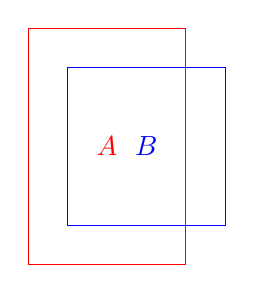
\begin{tikzpicture}
                    \draw[red] (0, 0) -- (2, 0) -- (2, 3) -- (0, 3) -- cycle;
                    \node[red] at (1, 1.5) {$A$};

                    \draw[blue] (0.5, 0.5) -- (2.5, 0.5) -- (2.5, 2.5) -- (0.5, 2.5) -- cycle;
                    \node[blue] at (1.5, 1.5) {$B$};
                \end{tikzpicture}
            \end{center}
            We consider the detection of the intersection over union (IoU) is above $0.5$;
            $$\text{IoU} = \frac{\red{A} \cap \blue{B}}{\red{A} \cup \blue{B}} > 0.5$$
            Another more complex piece of information we can extract is to perform \textbf{image segmentation}, allowing us to draw contours for each object.
            \subsubsection*{Applications}
                Computer vision is used in our lives daily;
                \begin{itemize}
                    \itemsep0em
                    \item \textbf{face detection}
                        \smallskip

                        This can be noticed in most camera applications on modern smartphones, when a small box is drawn around faces.
                        The algorithm first extracts \textbf{Haar} features from an image, and then determines (with these features) whether a region is a face or not.
                        \medskip

                        One example of these features is checking the contrast between the eyes and nose (horizontally); as the eyes tend to be quite dark in comparison.
                        Another contrast is checked, this time between your eyes, as the nose tends to be brighter.
                    \item \textbf{automatic number plate recognition}
                        \smallskip

                        Automated barriers in parking lots can read number plates in order to calculate how long a car stays.
                        Similarly, this can also be used to recognise building numbers, which is overlaid onto \textit{Google Maps}, allowing for a large database of street numbers to be built in an automated fashion.
                    \item \textbf{autonomous driving}
                    \item \textbf{image style transfer}
                        \smallskip

                        \textit{Choi et al. StarGAN: Unified Generative Adversarial Networks for Multi-Domain Image-to-Image Translation} - used for changing features on inputs.
                        Related to face motion capture (see \textit{Face2Face}).
                        Also see \textit{DeepFake}.
                    \item \textbf{Kinect}
                        \smallskip

                        Works by taking a depth image, segmenting it into body parts, locating key points and building a skeleton.
                    \item \textbf{design}
                        \smallskip

                        See \textit{OpenAI}'s \textit{DALL-E}, combining NLP and computer vision by generating images based on the concepts of words in a sentence.
                    \item \textbf{healthcare}
                        \smallskip

                        Medical image analysis can be used for disease diagnosis.
                        For example, identifying breast cancer lesions from mammograms.
                \end{itemize}
        \subsection*{Lecture 2 - Image Formation}
            An image, in RGB format, can be represented as pixels, each being three numbers.
            A digital image is formed from a lighting source being reflected into an optics sensor (eyes, cameras, etc).
            \subsubsection*{Light}
                A \textbf{point light source} originates from a single location in space, such as a small light bulb, or the sun.
                This can be described with three properties; location, intensity, and the spectrum.
                \medskip

                On the other hand, an \textbf{area light source} is more complex.
                For example, this could be a ceiling light; a rectangle of point lights.
            \subsubsection*{Reflectance}
                When light emitted from the source hits the surface of an object, it will be reflected.
                To describe this, we typically use the \textbf{bidirectional reflectance distribution function (BDRF)} to model this behaviour (where $\lambda$ is the wavelength, $L_r$ is the output power, and $E_i$ is the input power);
                $$f_r(\underbrace{\theta_i, \varphi_i}_\text{incident}, \underbrace{\theta_r, \varphi_r}_\text{reflected}, \lambda) = \dif{L_r}{E_i}$$
                While this is a very general model, it is very complex.
                \medskip

                As such, we can use \textbf{diffuse reflection}, where light is assumed to be scattered uniformly in all directions.
                This has a constant BRDF - this says that regardless of the incident or reflected directions, nor the wavelength, the power will be constant;
                $$f_r(\theta_i, \varphi_i, \theta_r, \varphi_r,, \lambda) = f_r(\lambda)$$
                \begin{center}
                    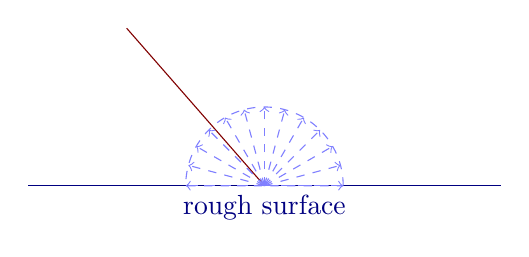
\begin{tikzpicture}
                        \draw[blue!50!black] (0, 0) edge[below] node{rough surface} (6, 0);
                        \draw[red!50!black] (1.25, 2) edge[->] (3, 0);
                        \draw[dashed, blue!50]
                        (4, 0) arc(0:180:1) -- cycle
                        (3, 0) edge[->] +(0:1)
                        (3, 0) edge[->] +(15:1)
                        (3, 0) edge[->] +(30:1)
                        (3, 0) edge[->] +(45:1)
                        (3, 0) edge[->] +(60:1)
                        (3, 0) edge[->] +(75:1)
                        (3, 0) edge[->] +(90:1)
                        (3, 0) edge[->] +(105:1)
                        (3, 0) edge[->] +(120:1)
                        (3, 0) edge[->] +(135:1)
                        (3, 0) edge[->] +(150:1)
                        (3, 0) edge[->] +(165:1)
                        (3, 0) edge[->] +(180:1);
                    \end{tikzpicture}
                \end{center}
                On the other hand, we can use \textbf{specular reflection} which performs reflections in a mirror-like fashion.
                The reflection and incident directions are symmetric with respect to the surface normal $\vec{n}$, such that $\theta_r = \theta_i$, with the same amount of power;
                \begin{center}
                    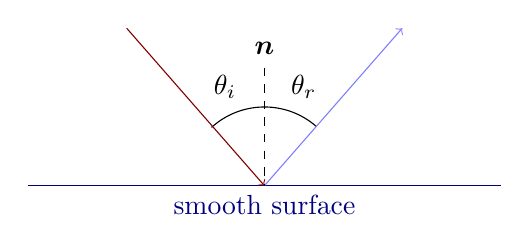
\begin{tikzpicture}
                        \draw (3, 0) ++(48.8:1) arc (48.8:132.2:1);
                        \draw[blue!50!black] (0, 0) edge[below] node{smooth surface} (6, 0);
                        \draw[red!50!black] (1.25, 2) edge[->] (3, 0);
                        \draw[blue!50] (4.75, 2) edge[<-] (3, 0);
                        \draw[dashed] (3, 1.5) -- (3, 0);

                        \node at (3, 1.75) {$\vec{n}$};
                        \node at (2.5, 1.25) {$\theta_i$};
                        \node at (3.5, 1.25) {$\theta_r$};
                    \end{tikzpicture}
                \end{center}
                While these two are the \textbf{ideal} cases, the majority of cases, we see a combination of both of those, as well as \textbf{ambient} illumination.
                Ambient illumination accounts for general illumination which could be complicated to model.
                For example, these could be repeated reflections between walls (which would be very difficult to calculate), and we instead assume that there is some light that exists in the 3D space representing the room.
                Another example could be a distance source, such as the sky (which has atmosphere).
                \medskip

                Combining these, we can use the \textbf{Phong} reflection model.
                This is an empirical model that describes how a surface reflects light as a combination of ambient, diffuse, and specular components.
            \subsubsection*{`Duality' with Computer Graphics}
                Using the game engine to produce example images is useful, as we are able to directly obtain the labels of objects from the engine itself, as well as visual output.
                As such, we can use these images as training for a model, since we also have an associated label map.
                This synthetic data is complementary to time-consuming manual annotations.
            \subsubsection*{Optics and Sensors}
                Both our eyes and cameras work in similar ways, with a lens governed by the thin lens equation, where $f$ denotes the focal length of the lens, $u$ denotes the distance from the subject to the lens, and $v$ denotes the distance from the lens to the image;
                $$\frac{1}{f} = \frac{1}{u} + \frac{1}{v}$$
                Our eyes work by light rays being focused by the cornea and lens onto the retina, where vision begins with two neural cells.
                The \textbf{cone} cells are responsible for colour vision, and function in bright light.
                On the other hand, the \textbf{rod} cells have little role in colour vision, but function in dim light.
                \medskip

                Humans have three types of cone cells (\textbf{trichromatic vision}), which have different response curves.
                The short cone cells respond to short wavelength lights (\violet{violet}, \blue{blue}), whereas the medium cone cells respond to medium wavelength lights (\textcolor{green}{green}), and long cone cells respond to long wavelength lights (\red{red}).
                Occasionally, there may be two cone cells, or four, which are referred to as \textbf{dichromacy} or \textbf{tetrachromacy} respectively.
                \medskip

                Note that colours are not objective physical properties of light or electromagnetic wave (which have a physical property of wavelength).
                Colour is a subjective feature, dependent on the visual perception of the observer.
                Since \textbf{rod} cells are more sensitive to light, they are the primary source of visual information at night.
                \medskip

                On the other hand, camera sensors have two common types;
                \begin{itemize}
                    \itemsep0em
                    \item \textbf{CCD} (charged-coupled device) \hfill often used in handheld cameras
                    \item \textbf{CMOS} (complementary metal-oxide semiconductor) \hfill used by most smartphone cameras
                \end{itemize}
                These sensors convert incoming light into electron charges, which are then read.
                \textbf{Bayer} filter arrays are a way to arrange RGB filters on sensors, half of which are green, and the remaining two quarters are red and blue.
                This mimics the human eyes, which are most sensitive to green light;
                \begin{center}
                    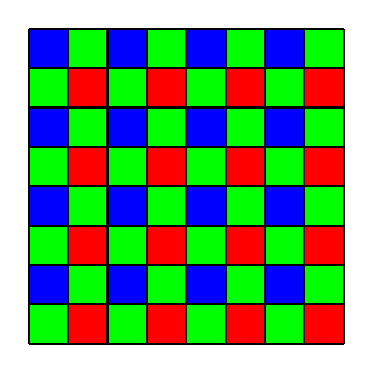
\begin{tikzpicture}[x=0.5cm, y=-0.5cm] % I should've just taken a screenshot, why do I keep doing this to myself
                        \foreach \i in {0,...,7} {
                            \foreach[evaluate={
                                \g=int(mod(\i + \j, 2);
                                \jm=int(mod(\j, 2))
                            }] \j in {0,...,7} {
                                \ifthenelse{\g = 1}
                                    {\def\col{green}}
                                    {\ifthenelse{\jm = 0}
                                        {\def\col{blue}}
                                        {\def\col{red}}}
                                \draw[fill=\col, draw=none] (\i, \j) -- (\i + 1, \j) -- (\i + 1, \j + 1) -- (\i, \j + 1) -- cycle;
                            }
                        }
                        \foreach \x in {0,...,8} {\draw[thick] (\x, 0) -- (\x, 8);}
                        \foreach \y in {0,...,8} {\draw[thick] (0, \y) -- (8, \y);}
                    \end{tikzpicture}
                \end{center}
                CMOS works by having sensors underneath each of these filtered portions, which can report an electrical signal.
                However, note that only one colour is available at each pixel (therefore the rest must be interpolated from the neighbours, by using bilinear interpolation; which simply averages the 4 neighbours).
                For example, consider the following pixel (denoted as a white cross);
                \begin{center}
                    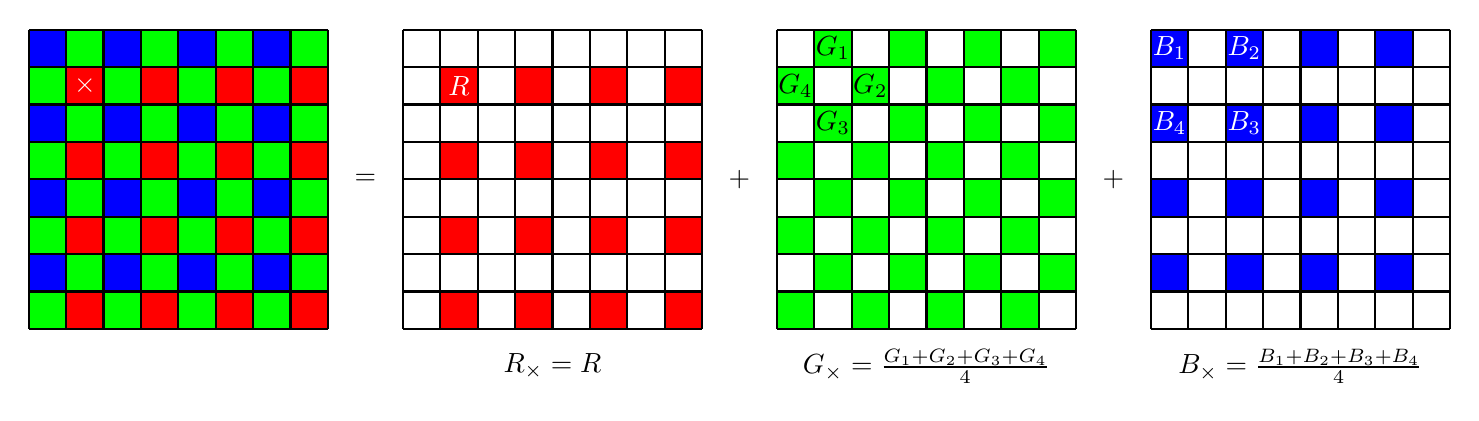
\begin{tikzpicture}[x=0.475cm, y=-0.475cm] % I should've just taken a screenshot, why do I keep doing this to myself
                        \begin{scope}[shift={(0, 0)}]
                            \foreach \i in {0,...,7} {
                                \foreach[evaluate={
                                    \g=int(mod(\i + \j, 2);
                                    \jm=int(mod(\j, 2))
                                }] \j in {0,...,7} {
                                    \ifthenelse{\g = 1}
                                        {\def\col{green}}
                                        {\ifthenelse{\jm = 0}
                                            {\def\col{blue}}
                                            {\def\col{red}}}
                                    \draw[fill=\col, draw=none] (\i, \j) -- (\i + 1, \j) -- (\i + 1, \j + 1) -- (\i, \j + 1) -- cycle;
                                }
                            }
                            \foreach \x in {0,...,8} {\draw[thick] (\x, 0) -- (\x, 8);}
                            \foreach \y in {0,...,8} {\draw[thick] (0, \y) -- (8, \y);}

                            \node[white] at (1.5, 1.5) {$\times$};
                        \end{scope}
                        \begin{scope}[shift={(10, 0)}]
                            \foreach \i in {0,...,7} {
                                \foreach[evaluate={
                                    \g=int(mod(\i + \j, 2);
                                    \jm=int(mod(\j, 2))
                                }] \j in {0,...,7} {
                                    \ifthenelse{\g = 1}
                                        {\def\col{white}}
                                        {\ifthenelse{\jm = 0}
                                            {\def\col{white}}
                                            {\def\col{red}}}
                                    \draw[fill=\col, draw=none] (\i, \j) -- (\i + 1, \j) -- (\i + 1, \j + 1) -- (\i, \j + 1) -- cycle;
                                }
                            }
                            \foreach \x in {0,...,8} {\draw[thick] (\x, 0) -- (\x, 8);}
                            \foreach \y in {0,...,8} {\draw[thick] (0, \y) -- (8, \y);}

                            \node[white] at (1.5, 1.5) {$R$};
                        \end{scope}
                        \begin{scope}[shift={(20, 0)}]
                            \foreach \i in {0,...,7} {
                                \foreach[evaluate={\g=int(mod(\i + \j, 2)}] \j in {0,...,7} {
                                    \ifthenelse{\g = 1}
                                        {\def\col{green}}
                                        {\def\col{white}}
                                    \draw[fill=\col, draw=none] (\i, \j) -- (\i + 1, \j) -- (\i + 1, \j + 1) -- (\i, \j + 1) -- cycle;
                                }
                            }
                            \foreach \x in {0,...,8} {\draw[thick] (\x, 0) -- (\x, 8);}
                            \foreach \y in {0,...,8} {\draw[thick] (0, \y) -- (8, \y);}

                            \node at (1.5, 0.5) {$G_1$};
                            \node at (2.5, 1.5) {$G_2$};
                            \node at (1.5, 2.5) {$G_3$};
                            \node at (0.5, 1.5) {$G_4$};
                        \end{scope}
                        \begin{scope}[shift={(30, 0)}]
                            \foreach \i in {0,...,7} {
                                \foreach[evaluate={
                                    \g=int(mod(\i + \j, 2);
                                    \jm=int(mod(\j, 2))
                                }] \j in {0,...,7} {
                                    \ifthenelse{\g = 1}
                                        {\def\col{white}}
                                        {\ifthenelse{\jm = 0}
                                            {\def\col{blue}}
                                            {\def\col{white}}}
                                    \draw[fill=\col, draw=none] (\i, \j) -- (\i + 1, \j) -- (\i + 1, \j + 1) -- (\i, \j + 1) -- cycle;
                                }
                            }
                            \foreach \x in {0,...,8} {\draw[thick] (\x, 0) -- (\x, 8);}
                            \foreach \y in {0,...,8} {\draw[thick] (0, \y) -- (8, \y);}

                            \node[white] at (0.5, 0.5) {$B_1$};
                            \node[white] at (2.5, 0.5) {$B_2$};
                            \node[white] at (2.5, 2.5) {$B_3$};
                            \node[white] at (0.5, 2.5) {$B_4$};
                        \end{scope}
                        \node at (9, 4) {$=$};
                        \node at (19, 4) {$+$};
                        \node at (29, 4) {$+$};

                        \node at (14, 9) {$R_\times = R$};
                        \node at (24, 9) {$G_\times = \frac{G_1 + G_2 + G_3 + G_4}{4}$};
                        \node at (34, 9) {$B_\times = \frac{B_1 + B_2 + B_3 + B_4}{4}$};
                    \end{tikzpicture}
                \end{center}
                Note that the use of different filters, and this interpolation, can lead to slightly different colours between cameras.
            \subsubsection*{Image Representation}
                The earliest colour space was described in 1931 by CIE, by performing a colour matching experiment.
                In this experiment, an observer attempts to match different levels of red, green, and blue lights to match a target light.
                This allows for colours to be represented in 3D space, as $(X, Y, Z)$, corresponding to the different levels.
                Colours can also be represented on a 2D plane, by normalising brightness;
                \begin{align*}
                    x & = \frac{X}{X + Y + Z} \\
                    y & = \frac{Y}{X + Y + Z} \\
                    z & = \frac{Z}{X + Y + Z} \\
                    & = 1 - x - y & \text{therefore redundant}
                \end{align*}
                Here $X, Y, Z$ are primary colours ($R, G, B$), and $x, y$ are chromacity / colour after removing brightness.
                This is much easier to draw.
                However, this colour space, also known as the \textbf{gamut} of human vision, was invented before computer screens.
                \medskip

                The sRGB (standard RGB) space was created by \textit{HP} and \textit{Microsoft} in 1996 for use on monitors, printers, and the internet.
                \begin{center}
                    \begin{tabular}{lcc}
                        sRGB definition & $x$ & $y$ \\
                        \hline
                        \red{red} & 0.64 & 0.33 \\
                        \textcolor{green}{green} & 0.30 & 0.60 \\
                        \blue{blue} & 0.15 & 0.06
                    \end{tabular}
                \end{center}
                This is represented by a triangle (which is a subset) in the gamut of human vision.
                As this is a subset, it cannot produce all the colours visible by the human eye.
                \medskip

                There are other colour spaces, such as HSV, CMYK, and so on.
                Note that CMYK is a \textbf{subtractive} colour model, starting from white, whereas RGB is an \textbf{additive} colour model, where we start from black.
                There can also be an alpha channel in RGB, which represents transparency.
                In a greyscale image, the three components are equal, hence only require one number.
            \subsubsection*{Quantisation}
                Note that this is covered in lecture 3.
                \medskip

                \textbf{Quantisation} maps a continuous signal to a discrete signal.
                The pictures from a camera are a continuous signal, but when it is stored on the camera, it is quantised to a discrete signal.
                Numerical errors can occur during this process, and the magnitude of the errors depends on the number of bits used (less error with more bits; 16 bits can store from 0 to 65535, compared to 8 bits storing from 0 to 255).
                \medskip

                Physically, an analog-to-digital convert (ADC) is used to perform the conversion.
                The energy of photons are converted into voltage, amplified, and then converted.
            \subsubsection*{Compression}
                In order to reduce the cost of storage to transmission, compression may be used.
                Lossy compression loses information after the compression (such as discrete cosine transform (DCT) in JPEG, often used for images or videos).
                However, lossless compression can also reduce the file size (less efficient compared to lossy), and is preferred for archival purposes or important imaging, where detail needs to be recovered.
        \subsection*{Lecture 3 - Image Filtering I}
            Note that in this course, most of the examples will be done on greyscale images, but can be applied to the channels individually.
            Some examples of filters include;
            \begin{itemize}
                \itemsep0em
                \item identity filter
                    \smallskip

                    Does nothing to the image.
                \item low-pass / smoothing (moving average, Gaussian)
                    \smallskip

                    Removes high-frequency signals, and keep low-frequency signals.
                \item high-pass / sharpening
                    \smallskip

                    Similar to the previous filter (keeps high-frequency signals, and removes low-frequency).
                \item denoise (median, non-local means, block-matching and 3D filtering)
            \end{itemize}
            \subsubsection*{Moving Average Filter}
                This is commonly used for 1D signal processing (time series), such as stocks, which can be quite noisy.
                To smooth out a noisy curve, it moves a window across the signal (and calculates the average value within the window) - the larger the window size, the smoother the result.
                \medskip

                In a two dimensional case, we can use a \textbf{filter kernel} (for example, with a $3 \times 3$ kernel);
                $$\frac{1}{9} \begin{bmatrix}
                    1 & 1 & 1 \\
                    1 & 1 & 1 \\
                    1 & 1 & 1
                \end{bmatrix}$$
                At each pixel, we apply the kernel centred at the pixel, and take the average of the pixels around it (and itself) to create a new output image.
                When we blur with a larger kernel, such as $7 \times 7$, we end up with a blurrier image.
                Note that the output image is smaller than the input image.
                We can pad the image with zeroes (anything outside of the picture is 0), or by mirroring the pixels (copying the boundary pixels).
                \medskip

                Consider an image of size $N \times N$, and a kernel size of $K \times K$.
                At each pixel, we perform $K^2$ multiplications (by the kernel weights), and then $K^2 - 1$ summations.
                This has to be done for each pixel, hence $N^2$ times.
                Therefore this results in $N^2 K^2$ multiplications and $N^2 (K^2 - 1)$ summations; giving a \textbf{complexity} of $O(N^2 K^2)$.
                However, we'd like to reduce this, if possible.
                \medskip

                If a big filter can be separated as two filters (\textbf{separable filter}) applied consecutively, we can perform the first operation, and then the second.
                An average in a 2D window can be done as an average across rows (horizontal), and then an average across columns (vertical);
                $$\begin{bmatrix}
                    \frac{1}{9} & \frac{1}{9} & \frac{1}{9} \\
                    \frac{1}{9} & \frac{1}{9} & \frac{1}{9} \\
                    \frac{1}{9} & \frac{1}{9} & \frac{1}{9}
                \end{bmatrix} = \begin{bmatrix}
                    \frac{1}{3} & \frac{1}{3} & \frac{1}{3}
                \end{bmatrix} * \begin{bmatrix}
                    \frac{1}{3} \\ \frac{1}{3} \\ \frac{1}{3}
                \end{bmatrix}$$
                Doing these two filters, we end up with an equivalent result to the original 2D filter.
                Note that $*$ is a convolution (see next lecture).
                \medskip

                Consider the complexity of separable filtering.
                The image size remains as $N \times N$, however we have two kernels, of $1 \times K$ and $K \times 1$ respectively.
                At each pixel we do $K$ multiplications followed by $K - 1$ summations.
                Again, this is done for $N^2$ pixels, and twice (once for each filter).
                Therefore, the total number of multiplications is $2N^2K$ multiplications and $2N^2(K - 1)$ summations.
                This is better, in contrast to the original complexity, as we have complexity of $O(N^2K)$ - which will make a difference for large $K$.
                \medskip

                A moving average filter removes high frequency signals (noise or sharpness), which results in a smooth but blurry image.
            \subsubsection*{Gaussian Filter}
                The kernel is a 2D Gaussian distribution;
                $$h(i, j) = \frac{1}{2 \pi \sigma^2} e^{-\frac{i^2 + j^2}{2 \sigma^2}}$$
                Here we have $i, j = 0, 0$ as the centre of the kernel.
                While the support is infinite, small values outside the range $[-k\sigma, k\sigma]$ can be ignored (very small values, such as $k=3$ or $k=4$).
                Note that $\sigma$ is a manually defined parameter.
                This is a separable filter, which is equivalent to two 1D Gaussian filters with the same $\sigma$, with one along the $x$-axis and the other along the $y$-axis;
                \begin{align*}
                    h(i, j) & = h_x(i) * h_y(j) \\
                    h_x(i) & = \frac{1}{\sqrt{2 \pi \sigma^2}} e^{-\frac{i^2}{2\sigma^2}}
                \end{align*}
            \subsubsection*{High-pass Filter}
                One design is to do the following;
                $$\underbrace{\begin{bmatrix}
                    0 & 0 & 0 \\
                    0 & 1 & 0 \\
                    0 & 0 & 0
                \end{bmatrix}}_\text{identity} + \underbrace{\left(\begin{bmatrix}
                    0 & 0 & 0 \\
                    0 & 1 & 0 \\
                    0 & 0 & 0
                \end{bmatrix} - \begin{bmatrix}
                    \frac{1}{9} & \frac{1}{9} & \frac{1}{9} \\
                    \frac{1}{9} & \frac{1}{9} & \frac{1}{9} \\
                    \frac{1}{9} & \frac{1}{9} & \frac{1}{9}
                \end{bmatrix}\right)}_\text{high-frequency} = \begin{bmatrix}
                    -\frac{1}{9} & -\frac{1}{9} & -\frac{1}{9} \\
                    -\frac{1}{9} & \frac{17}{9} & -\frac{1}{9} \\
                    -\frac{1}{9} & -\frac{1}{9} & -\frac{1}{9}
                \end{bmatrix}$$
                We can add a high frequency signal to the identity, in order to enhance it.
            \subsubsection*{Median Filter}
                This is a non-linear filter (not performing an average calculation by multiplication).
                This moves a sliding window, and replaces the centre pixel with the median value in the window - this is not a linear equation.
        \subsection*{Lecture 4 - Image Filtering II}
            \subsubsection*{Mathematical Description}
                Consider a simple filter, of size 3, in 1D.
                With an input $f$, and an output $g$, it can be written as the weighted average in a window;
                $$g[n] = \frac{1}{3} f[n - 1] + \frac{1}{3} f[n] + \frac{1}{3} f[n + 1]$$
                In general, filtering takes in an input signal $f$, processes it and generates an output signal $g$.
                A filter is a device (or process) that removes unwanted components or features from a signal (keeps / enhances wanted filters).
                \medskip

                In order to mathematically describe a filter, we need the concept of \textbf{impulse response}; the output of a  filter when the input is an \textbf{impulse signal} (only have a signal at a single time point);
                \begin{center}
                    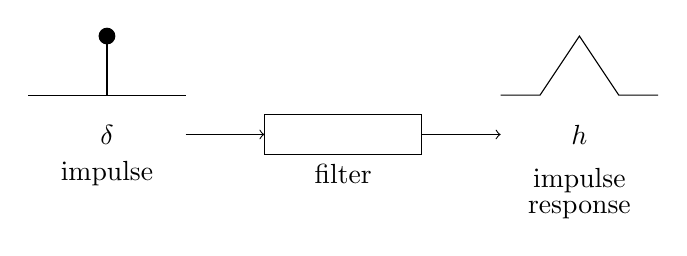
\begin{tikzpicture}
                        \begin{scope}
                            \draw (0, 0) -- (2, 0);
                            \draw (1, 0) -- (1, 0.75);
                            \node[rbtb] at (1, 0.75) {};
                            \node at (1, -0.5) {$\delta$};
                            \node at (1, -1) {impulse};
                        \end{scope}
                        \draw (2, -0.5) edge[->] (3, -0.5);
                        \draw (5, -0.5) edge[->] (6, -0.5);
                        \draw (3, -0.25) -- (5, -0.25) -- (5, -0.75) -- (3, -0.75) -- cycle;
                        \node at (4, -1) {filter};
                        \begin{scope}[shift={(6, 0)}]
                            \draw (0, 0) -- (0.5, 0) -- (1, 0.75) -- (1.5, 0) -- (2, 0);
                            \node at (1, -0.5) {$h$};
                            \node at (1, -1.25) {\shortstack{impulse\\response}};
                        \end{scope}
                    \end{tikzpicture}
                \end{center}
                For a continuous signal, we treat an impulse as a Dirac delta function $\delta(x)$, whereas for a discrete signal, we treat an impulse as a Kronecker delta function $\delta[i]$;
                \begin{align*}
                    \delta(x) & = \begin{cases}
                        \infty & \text{if } x = 0 \\
                        0 & \text{otherwise}
                    \end{cases} \\
                    \defint{-\infty}{\infty}{\delta(x)}{x} & = 1 \\
                    \delta[i] & = \begin{cases}
                        1 & \text{if } i = 0 \\
                        0 & \text{otherwise}
                    \end{cases}
                \end{align*}
                The impulse response $h$ completely characterises a \textbf{linear time-invariant} filter.
                Note that we can consider a filter as time-invariant if, by shifting the input signal some number of time steps $k$, the output signal will remain the same (shape and values) but shifted by the \textbf{same} number of time steps.
                For example;
                \begin{itemize}
                    \itemsep0em
                    \item $g[n] = 10 \cdot f[n]$ is time-invariant and amplifies the input by a constant
                    \item $g[n] = n \cdot f[n]$ is \textbf{not} time-invariant since the amount it amplifies the input depends on the time step $n$
                \end{itemize}
                As long as we know $h$, and have an input $x$, we can calculate the output signal $y$.
                Since it uniquely describes a filter, we often denote a filter by its impulse response function $h$.
                \medskip

                Additionally, a filter can be \textbf{linear}.
                If it is a linear system, when two input signals are combined linearly, their outputs will also be combined linearly.
                Let $f_1[n]$ lead to an output $g_1[n]$, and $f_2[n]$ to $g_2[n]$.
                $$\text{output}(\alpha f_1[n] + \beta f_2[n]) = \alpha g_1[n] + \beta g_2[n]$$
            \subsubsection*{Convolution}
                Most of the filters we've previously covered are linear time-invariant.
                Since $h$ characterises how the system works (as it is linear time-invariant), it's possible for the output $g$ to be described as the \textbf{convolution} between an input $f$ and impulse response $h$;
                $$g[n] = f[n] * h[n]$$
                \medskip

                We can describe an input signal $f[n]$ as the following, where each time step is a constant multiplied by a spike;
                $$f[n] = f[0]\delta[n] + f[1]\delta[n - 1] + f[2]\delta[n - 2] + f[3]\delta[n - 3] + \dots$$
                However, since we know the output of $\delta[n]$ is $h[n]$, we can write the output as;
                $$g[n] = f[0]h[n] + f[1]h[n - 1] + f[2]h[n - 2] + f[3]h[n - 3] + \dots$$
                The output mathematical operation is defined as a convolution, where a signal $f$ and a filter with impulse response / convolution kernel $h$ is defined as;
                $$g[n] = f[n] * h[n] = \summation{m = -\infty}{\infty} f[m]h[n - m]$$
                The continuous form (previously we have only considered the discrete form);
                $$g(t) = f(t) * h(t) = \defint{-\infty}{\infty}{f(\tau) h(t - \tau)}{\tau}$$
                Focusing on the discrete case, we notice the following (when we replace $m$ with $n - m$);
                $$\summation{m = -\infty}{\infty} f[m]h[n - m] = \summation{m = -\infty}{\infty} f[n - m]h[m]$$
                This shows that the convolution of $f$ and $h$ is equivalent to the convolution of $h$ and $f$ (commutativity);
                $$f[n] * h[n] = h[n] * f[n]$$
                By expanding the equations, we can also show that convolution satisfies associativity, such that;
                $$f * (g * h) = (f * g) * h$$
                We also have distributivity;
                $$f * (g + h) = (f * g) + (f * h)$$
                And also differentiation;
                $$\dif{}{x}(f * g) = \dif{f}{x} * g = f * \dif{g}{x}$$
                With a more concrete example, we can visualise it as follows (this is the moving average of size 3);
                \begin{center}
                    \begin{tikzpicture}
                        \begin{scope}[shift={(0, 1.5)}]
                            \draw (1, 0) -- (4, 0) -- (4, -1) -- (1, -1) -- cycle;
                            \foreach \i in {1,...,2} {
                                \draw (\i + 1, 0) -- (\i + 1, -1);
                            }
                            \node at (1.5, -0.5) {\tiny $h[1]$};
                            \node at (2.5, -0.5) {\tiny $h[0]$};
                            \node at (3.5, -0.5) {\tiny $h[-1]$};
                        \end{scope}

                        \draw (0, 0) -- (6, 0) -- (6, -1) -- (0, -1) -- cycle;
                        \foreach \i in {1,...,5} {
                            \draw (\i, 0) -- (\i, -1);
                        }
                        \node at (1.5, -0.5) {\tiny$f[n - 1]$};
                        \node at (2.5, -0.5) {\tiny$f[n]$};
                        \node at (3.5, -0.5) {\tiny$f[n + 1]$};

                        \draw (8, 0) -- (14, 0) -- (14, -1) -- (8, -1) -- cycle;
                        \foreach \i in {1,...,5} {
                            \draw (\i + 8, 0) -- (\i + 8, -1);
                        }
                        \node at (10.5, -0.5) {\tiny$g[n]$};
                    \end{tikzpicture}
                \end{center}
                In our case, we have the kernel $h[n]$, and the values;
                \begin{align*}
                    h[-1] & = \frac{1}{3} \\
                    h[0] & = \frac{1}{3} \\
                    h[1] & = \frac{1}{3} \\
                    h[n] & = \begin{bmatrix}
                        \frac{1}{3}, & \frac{1}{3}, & \frac{1}{3}
                    \end{bmatrix}
                \end{align*}
                This can be expanded into the 2D case, which is used for image filtering;
                $$g[m, n] = f[m, n] * h[m, n] = \summation{i = -\infty}{\infty} \summation{j = -\infty}{\infty} f[i, j] h[m - i, n - j]$$
                This can also be written as the following, replacing $m - i, n - j$ by $i, j$;
                $$g[m, n] = \summation{i = -\infty}{\infty} \summation{j = -\infty}{\infty} f[m - i, n - j] h[i, j]$$
                By using the property of associativity, if a big filter (call it $f_b$) can be written as the convolution of $g$ and $h$ (smaller filters), we can first convolve $f$ with $g$, then with $h$ - this is used for separable filtering;
                $$f * f_b = f * (g * h) = (f * g) * h$$
                For example (note that we have padded zeroes, but in code we do not need that);
                $$\underbrace{\begin{bmatrix}
                    \frac{1}{9} & \frac{1}{9} & \frac{1}{9} \\
                    \frac{1}{9} & \frac{1}{9} & \frac{1}{9} \\
                    \frac{1}{9} & \frac{1}{9} & \frac{1}{9}
                \end{bmatrix}}_{f_b} = \underbrace{\begin{bmatrix}
                    \textcolor{black!33}{0} & \textcolor{black!33}{0} & \textcolor{black!33}{0} \\
                    \frac{1}{3} & \frac{1}{3} & \frac{1}{3} \\
                    \textcolor{black!33}{0} & \textcolor{black!33}{0} & \textcolor{black!33}{0}
                \end{bmatrix}}_{g} * \underbrace{\begin{bmatrix}
                    \textcolor{black!33}{0} & \frac{1}{3} & \textcolor{black!33}{0} \\
                    \textcolor{black!33}{0} & \frac{1}{3} & \textcolor{black!33}{0} \\
                    \textcolor{black!33}{0} & \frac{1}{3} & \textcolor{black!33}{0}
                \end{bmatrix}}_{h}$$
        \subsection*{Lecture 5 - Edge Detection I}
            \subsubsection*{Importance of Edges}
                In computer vision an edge refers to lines where image brightness changes sharply with discontinuities.
                This may be due to different reasons such as discontinuities in colour, depth, surface normals, etc.
                Edges capture important properties of what we see in the world, and they are important features for image analysis (for example, we first capture edges, then facial features, and so on).
                \textit{Hubel} and \textit{Wiesel} performed vision experiments in 1959, finding that neuron cells in the primary visual cortex are orientation selective, responding strongly to lines or edges of a particular orientation.
                Humans can also read images even if reduced to simple line drawings.
                Edges are also heavily used in convolutional networks, with the first layer tending to learn edges, with the later layers learning increasingly complex patterns.
            \subsubsection*{Detection}
                An image can be considered as a function of pixel positions (consider plotting the image on the $x-y$ axes, and having the $z$ axis denote intensity).
                Mathematically, derivatives characterise function discontinuities, which can be used to help edge detection.
                For a continuous function, the derivative is;
                $$f^\prime(x) = \limit{h}{0} \frac{f(x + h) - f(x)}{h}$$
                On the other hand, for a discrete function (finite difference);
                $$\underbrace{f^\prime[x] = f[x + 1] - f[x]}_\text{forward difference} \ \ \ \ \ \underbrace{f^\prime[x] = f[x] - f[x - 1]}_\text{backward difference} \ \ \ \ \ \underbrace{f^\prime[x] = \frac{f[x + 1] - f[x - 1]}{2}}_\text{central difference}$$
                Notice that these can also be performed with convolutions, using the following kernels;
                $$\underbrace{h = [1, -1, 0]}_\text{forward difference} \ \ \ \ \ \ \ \ \ \ \underbrace{h = [0, 1, -1]}_\text{backward difference} \ \ \ \ \ \ \ \ \ \  \underbrace{h = [1, 0, -1]}_\text{central difference}$$
            \subsubsection*{Prewitt and Sobel Filters}
                The Prewitt filters, along the $x$-axis (horizontal direction) and along the $y$-axis (vertical direction) are as follows;
                \begin{center}
                    \hfill
                    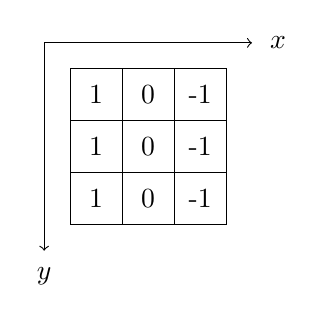
\begin{tikzpicture}[x=0.66cm, y=0.66cm]
                        \draw
                        (-0.5, 3.5) edge[->] (3.5, 3.5)
                        (-0.5, 3.5) edge[->] (-0.5, -0.5);
                        \node at (4, 3.5) {$x$};
                        \node at (-0.5, -1) {$y$};
                        \draw
                        (0, 0) -- (3, 0) -- (3, 3) -- (0, 3) -- cycle
                        (0, 1) -- (3, 1)
                        (0, 2) -- (3, 2)
                        (1, 0) -- (1, 3)
                        (2, 0) -- (2, 3);
                        \node at (0.5, 0.5) {1};
                        \node at (0.5, 1.5) {1};
                        \node at (0.5, 2.5) {1};
                        \node at (1.5, 0.5) {0};
                        \node at (1.5, 1.5) {0};
                        \node at (1.5, 2.5) {0};
                        \node at (2.5, 0.5) {-1};
                        \node at (2.5, 1.5) {-1};
                        \node at (2.5, 2.5) {-1};
                    \end{tikzpicture}
                    \hfill
                    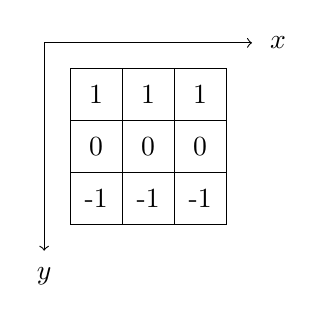
\begin{tikzpicture}[x=0.66cm, y=0.66cm]
                        \draw
                        (-0.5, 3.5) edge[->] (3.5, 3.5)
                        (-0.5, 3.5) edge[->] (-0.5, -0.5);
                        \node at (4, 3.5) {$x$};
                        \node at (-0.5, -1) {$y$};
                        \draw
                        (0, 0) -- (3, 0) -- (3, 3) -- (0, 3) -- cycle
                        (0, 1) -- (3, 1)
                        (0, 2) -- (3, 2)
                        (1, 0) -- (1, 3)
                        (2, 0) -- (2, 3);
                        \node at (0.5, 0.5) {-1};
                        \node at (0.5, 1.5) {0};
                        \node at (0.5, 2.5) {1};
                        \node at (1.5, 0.5) {-1};
                        \node at (1.5, 1.5) {0};
                        \node at (1.5, 2.5) {1};
                        \node at (2.5, 0.5) {-1};
                        \node at (2.5, 1.5) {0};
                        \node at (2.5, 2.5) {1};
                    \end{tikzpicture}
                    \hfill \phantom{}
                \end{center}
                Note that the Prewitt filter is a separable filter ([1] - moving average for smoothing);
                $$\underbrace{\begin{bmatrix}
                    1 & 0 & -1 \\
                    1 & 0 & -1 \\
                    1 & 0 & -1
                \end{bmatrix}}_\text{Prewitt filter} = \underbrace{\begin{bmatrix}
                    \textcolor{black!33}{0} & 1 & \textcolor{black!33}{0} \\
                    \textcolor{black!33}{0} & 1 & \textcolor{black!33}{0} \\
                    \textcolor{black!33}{0} & 1 & \textcolor{black!33}{0}
                \end{bmatrix}}_\text{[1]} * \underbrace{\begin{bmatrix}
                    \textcolor{black!33}{0} & \textcolor{black!33}{0} & \textcolor{black!33}{0} \\
                    1 & 0 & -1 \\
                    \textcolor{black!33}{0} & \textcolor{black!33}{0} & \textcolor{black!33}{0}
                \end{bmatrix}}_\text{finite difference}$$
                The Sobel filter is quite similar to the Prewitt filter;
                \begin{center}
                    \hfill
                    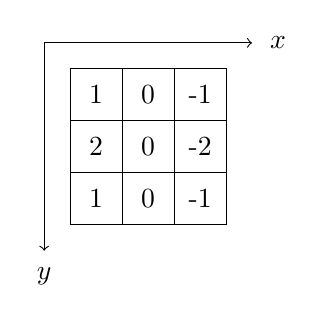
\begin{tikzpicture}[x=0.66cm, y=0.66cm]
                        \draw
                        (-0.5, 3.5) edge[->] (3.5, 3.5)
                        (-0.5, 3.5) edge[->] (-0.5, -0.5);
                        \node at (4, 3.5) {$x$};
                        \node at (-0.5, -1) {$y$};
                        \draw
                        (0, 0) -- (3, 0) -- (3, 3) -- (0, 3) -- cycle
                        (0, 1) -- (3, 1)
                        (0, 2) -- (3, 2)
                        (1, 0) -- (1, 3)
                        (2, 0) -- (2, 3);
                        \node at (0.5, 0.5) {1};
                        \node at (0.5, 1.5) {2};
                        \node at (0.5, 2.5) {1};
                        \node at (1.5, 0.5) {0};
                        \node at (1.5, 1.5) {0};
                        \node at (1.5, 2.5) {0};
                        \node at (2.5, 0.5) {-1};
                        \node at (2.5, 1.5) {-2};
                        \node at (2.5, 2.5) {-1};
                    \end{tikzpicture}
                    \hfill
                    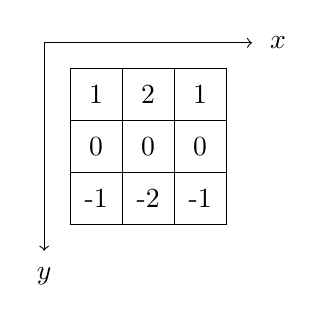
\begin{tikzpicture}[x=0.66cm, y=0.66cm]
                        \draw
                        (-0.5, 3.5) edge[->] (3.5, 3.5)
                        (-0.5, 3.5) edge[->] (-0.5, -0.5);
                        \node at (4, 3.5) {$x$};
                        \node at (-0.5, -1) {$y$};
                        \draw
                        (0, 0) -- (3, 0) -- (3, 3) -- (0, 3) -- cycle
                        (0, 1) -- (3, 1)
                        (0, 2) -- (3, 2)
                        (1, 0) -- (1, 3)
                        (2, 0) -- (2, 3);
                        \node at (0.5, 0.5) {-1};
                        \node at (0.5, 1.5) {0};
                        \node at (0.5, 2.5) {1};
                        \node at (1.5, 0.5) {-2};
                        \node at (1.5, 1.5) {0};
                        \node at (1.5, 2.5) {2};
                        \node at (2.5, 0.5) {-1};
                        \node at (2.5, 1.5) {0};
                        \node at (2.5, 2.5) {1};
                    \end{tikzpicture}
                    \hfill \phantom{}
                \end{center}
                Note that the Sobel filter is also a separable filter;
                $$\underbrace{\begin{bmatrix}
                    1 & 0 & -1 \\
                    2 & 0 & -2 \\
                    1 & 0 & -1
                \end{bmatrix}}_\text{Sobel filter} = \underbrace{\begin{bmatrix}
                    \textcolor{black!33}{0} & 1 & \textcolor{black!33}{0} \\
                    \textcolor{black!33}{0} & 2 & \textcolor{black!33}{0} \\
                    \textcolor{black!33}{0} & 1 & \textcolor{black!33}{0}
                \end{bmatrix}}_\text{smoothing} * \underbrace{\begin{bmatrix}
                    \textcolor{black!33}{0} & \textcolor{black!33}{0} & \textcolor{black!33}{0} \\
                    1 & 0 & -1 \\
                    \textcolor{black!33}{0} & \textcolor{black!33}{0} & \textcolor{black!33}{0}
                \end{bmatrix}}_\text{finite difference}$$
                Note that the outputs of the filters are different, with the horizontal filter detecting changes in the horizontal direction; describing discontinuity along the $x$-axis (leading to vertical lines).
                These can be combined to describe two properties of edges; the magnitude and the orientation.
                \begin{align*}
                    g_x & = f * h_x & \text{derivative along $x$-axis} \\
                    g_y & = f * h_y & \text{derivative along $y$-axis} \\
                    g & = \sqrt{g_x^2 + g_y^2} & \text{magnitude of the gradient} \\
                    \theta & = \mathrm{arctan2}(g_y, g_x) & \text{angle of the gradient}
                \end{align*}
            \subsubsection*{Derivative of Gaussian}
                Note that in both the filters above, there is some smoothing as derivatives are sensitive to noise (therefore the smoothing kernel helps to suppress noise).
                The Prewitt filters use the mean average kernel, whereas Sobel filters use the kernel $[1, 2, 1]$.
                Another option is to use the Gaussian kernel for smoothing, before calculating derivatives;
                $$h[x] = \frac{1}{\sqrt{2 \pi} \sigma}e^{-\frac{x^2}{2\sigma^2}}$$
                \medskip

                The derivative of Gaussian filter is an operation, performing Gaussian smoothing, before taking the derivative.
                However, recalling the rules for the differentiation of convolution, we have $f$ (input signal) convolved with the derivative of the Gaussian kernel;
                \begin{align*}
                    \dif{}{x}(f * h) & = f * \dif{h}{x} \\
                    & = f * \frac{-x}{\sqrt{2 \pi} \sigma^3} e^{-\frac{x^2}{2\sigma^2}}
                \end{align*}
                In the 2D case, the Gaussian filter is as follows;
                $$h[x, y] = \frac{1}{2 \pi \sigma^2}e^{-\frac{x^2 + y^2}{2 \sigma^2}}$$
                However, it is a separable filter (and therefore can be sped up) equivalent to the convolution of two 1D Gaussian filters.
                Notice there's a parameter $\sigma$ in the derivative of Gaussian.
                With a small $\sigma$, there is more detail in the magnitude map; on the other hand, a large $\sigma$ value suppresses noise and results in a smoother derivative.
                As such, different $\sigma$ values help to find edges at different scales.
        \subsection*{Lecture 6 - Edge Detection II}
            \subsubsection*{Canny Edge Detection}
                The results of the filters from the previous lectures (gradient magnitude map) have values ranging from black to white.
                However, we want either a 0 or 1 (black or white) - a \textbf{binary edge map}.
                \medskip

                There should be good detection; a low probability of failing too mark real edge points and low probability of falsely marking non-edge points.
                In addition, there should be good localisation - the points marked as edges should be as close as possible to the centre of the edge.
                Finally, there should only be a single response to a single edge.
                \medskip

                Canny edge detection is done in the following steps;
                \begin{enumerate}[1.]
                    \itemsep0em
                    \item perform Gaussian filtering to suppress noise
                        \smallskip

                        The choice of $\sigma$ depends on the type of edge we desire at the end.
                        If we want large edges (such as buildings), $\sigma$ should be set to a large value (such as 7).
                        However, if we want to pay attention to fine features, $\sigma$ can be set to a small value.
                    \item calculate gradient magnitudes and directions
                    \item apply non-maximum suppression (NMS) to get a single response for each edge
                        \smallskip

                        Non-maximum suppression aims to get a single response for each edge, by using the idea that the edge occurs where the gradient magnitude is maximum at the centre of the edge.
                        \begin{center}
                            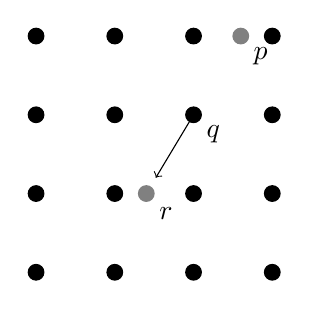
\begin{tikzpicture}
                                \foreach \x in {0,...,3} {
                                    \foreach \y in {0,...,3} {
                                        \node[rbtb] at (\x, \y) {};
                                    }
                                }
                                \node[inner sep=2pt, circle, draw=black!50, fill=black!50] at (2.6, 3) {};
                                \node[inner sep=2pt, circle, draw=black!50, fill=black!50] at (1.4, 1) {};
                                \node at (2.25, 1.75) {$q$};
                                \node at (2.85, 2.75) {$p$};
                                \node at (1.65, 0.75) {$r$};
                                \begin{scope}[shift={(2, 2)}, scale={0.8}]
                                    \draw (0, 0) edge[->] (-0.6, -1);
                                \end{scope}
                            \end{tikzpicture}
                        \end{center}
                        Compare the magnitude at $q$ with the magnitudes of $p$ and $r$, both along the gradient direction (in opposite directions).
                        If $q$ is the local maximum (larger than both $p$ and $r$), we keep the magnitude at pixel $q$.
                        $$M(x, y) = \begin{cases}
                            M(x, y) & \text{if local maximum} \\
                            0 & \text{otherwise}
                        \end{cases}$$
                        However, notice that there may be issues with $p$ and $r$ not being at exact pixel locations.
                        For example, using pixel $r$ (not at an integer position), we can perform interpolation.
                        It's possible to use linear interpolation (weighted by distance), or a simpler algorithm such as nearest neighbour interpolation (better performance).
                        Note that different interpolation algorithms will lead to different outcomes.
                        Another approach is to round the gradient direction into 8 possible angles, in steps of $45^\circ$ in the range $[0^\circ, 315^\circ]$, allowing us to check only along those directions to give exact pixels (intuitively quite similar to nearest neighbour).
                        \medskip

                        After NMS, there are fewer points with bright values.
                    \item perform hysteresis thresholding to find potential edges
                        \smallskip

                        Many pixels that are local maxima may still have very low magnitudes; however we only want edges with high magnitudes.
                        A simple thresholding would be to convert an intensity image to a binary image with a threshold $t$;
                        $$\text{binary}(x, y) = \begin{cases}
                            1 & \text{if } I(x, y) \geq t \\
                            0 & \text{otherwise}
                        \end{cases}$$
                        On the other hand, hysteresis thresholding defines two thresholds $t_\text{low}$ and $t_\text{high}$.
                        If the magnitude is $\geq t_\text{high}$, it is accepted as an edge pixel, and if it is $< t_\text{low}$, it is rejected.
                        However, if we have a value between the thresholds, we have a \textbf{weak edge} (which may or may not be an edge).
                        If it is connected to existing edge pixels, it is accepted, whereas if it is not connected (adjacent to one strong edge) to an existing edge, it will be rejected.
                \end{enumerate}
                The initial goals are satisfied as follows;
                \begin{itemize}
                    \itemsep0em
                    \item \textbf{good detection}
                        \smallskip

                        False positives are reduced by using Gaussian smoothing to suppress noise.
                        On the other hand, false negatives are reduced by using hysteresis thresholding to find weak edges.
                    \item \textbf{good localisation}
                        \smallskip

                        NMS finds locations based on gradient magnitude and direction.
                    \item \textbf{single response} \hfill also done with NMS
                \end{itemize}
            \subsubsection*{Learning-based Edge Detection}
                Decades of effort have been made to improve detection accuracy.
                This includes using richer features such as colour and texture, enforcing smoother, as well as using machine learning (by learning mapping from an image to edge directly from data).
                \medskip

                This machine learning algorithm assumes paired data (images $x$ and manually defined edge maps $y$).
                The problem finds a model (with model parameters $\theta$) that maps $x$ to $y$, such that $y = f(x\ |\ \theta)$.
                This differs from Canny edge detector, as our example integrates from multiple scales (fine-scale edges) with coarse-scale edges to form a final output.
                On the other hand, Canny edge detector uses a single scale for edge detection, controlled by a single parameter $\sigma$.
                \medskip

                An application for learning-based edge detection is to learn a mapping from a rough sketch to a simplified sketch.
                However, this isn't just an edge detection problem since it cannot be solved using NMS; when this is done by humans, a high-level understanding about the sketch is required.
            \subsubsection*{Conclusion}
                Edge detection is a fundamental problem in image processing and computer vision; aiming to identify where discontinuities occur, or identifying points that are edges.
                Two solutions are proposed;
                \begin{itemize}
                    \itemsep0em
                    \item if we know the explicit criteria, we can implement computational criteria
                    \item otherwise, we can collect data pairs representing what we want to achieve and train a machine learning model
                \end{itemize}
                Edges provide important low-level features both human vision and computer vision for understanding images.
                These algorithms provide ideas for other detection algorithms.
                \medskip

                We can also go in the other direction, taking edges to images.
                This aims to train a model that generates an image that looks close to real images, from edges.
                A model $G$ (generator) learns the mapping from edge to image.
                For example, we take an edge image $x$ to $G(x)$ (an image).
                A discriminator $d$ then attempts to assess whether the image is real or fake (GAN).
        \subsection*{Lecture 7 - Hough Transform}
            In the last lecture, we covered edge detection (1 for edge pixel, 0 for background).
            If we know these edges form some shape (such as a line), we want to obtain a parametric representation.
            \subsubsection*{Line Parameterisation}
                A line can be represented by two parameters (e.g. $m$ (slope) and $b$ ($y$-intercept)), which is much more efficient than a lot of edge points;
                \begin{itemize}
                    \itemsep0em
                    \item slope intercept form \hfill $m$ (slope) and $b$ ($y$-intercept)
                        $$y = mx + b$$
                    \item double intercept form \hfill $(a, 0)$ and $(0, b)$ are on the line
                        $$\frac{x}{a} + \frac{y}{b} = 1$$
                    \item normal form \hfill $\theta$ is angle and $\rho$ is distance
                        $$x\cos(\theta) + y\sin(\theta) = \rho$$
                \end{itemize}
            \subsubsection*{Hough Transform}
                Hough transform transforms from image space (edge map) to parameter space (two parameters of a line).
                The output is a parametric model, from a n input of edge points.
                Each edge point `votes' for possible models in the parameter space.
                One way is to fit a line model $(m, b)$ to the edge points $(x_1, y_1), (x_2, y_2), \dots$;
                $$\min_{m, b} \summation{i}{} (y_i - \underbrace{(mx_i + b)}_{\hat{y}})^2$$
                For the Hough transform we will use the slope intercept form.
                $$y = mx + b \Leftrightarrow b = y - mx$$
                Assume we have the edge points $(x_1, y_1), \dots$, each point will vote for a line model in the parameter space; for example, the first point votes for;
                $$b = y_1 - mx_1$$
                This can be seen graphically as the following (image space on the left, parameter space ($b = y - mx$) on the right);
                \begin{center}
                    \hfill
                    \begin{tikzpicture}
                        \begin{axis}[
                            axis on top=true,
                            axis line style=thick,
                            domain=-4:4, samples=9,
                            axis lines=middle, xlabel=$x$, ylabel=$y$,
                            height=8cm, width=8cm,
                            enlargelimits=false,
                            xtick={-4,-3,...,4},
                            ytick={-4,-3,...,4},
                            xmin=-4, xmax=4,
                            ymin=-4, ymax=4
                        ]
                            \node[label={45:{\tiny(3,3)}}, circle, fill=red, inner sep=2pt] at (axis cs:3,3) {};
                            \node[label={45:{\tiny(1,1)}}, circle, fill=green, inner sep=2pt] at (axis cs:1,1) {};
                            \node[label={135:{\tiny(-2,-2)}}, circle, fill=blue, inner sep=2pt] at (axis cs:-2,-2) {};
                        \end{axis}
                    \end{tikzpicture}
                    \hfill
                    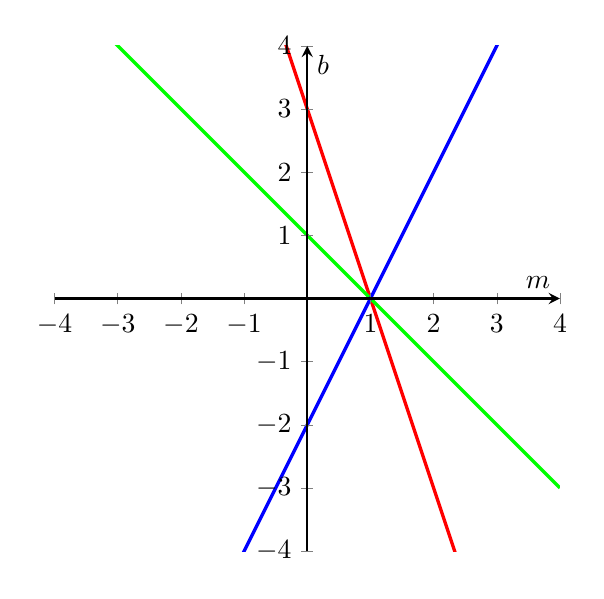
\begin{tikzpicture}
                        \begin{axis}[
                            axis on top=true,
                            axis line style=thick,
                            domain=-4:4, samples=9,
                            axis lines=middle, xlabel=$m$, ylabel=$b$,
                            height=8cm, width=8cm,
                            enlargelimits=false,
                            xtick={-4,-3,...,4},
                            ytick={-4,-3,...,4},
                            xmin=-4, xmax=4,
                            ymin=-4, ymax=4
                        ]
                            \addplot[very thick, red] {3 - 3*\x};
                            \addplot[very thick, green] {1 - \x};
                            \addplot[very thick, blue] {-2 + 2*\x};
                        \end{axis}
                    \end{tikzpicture}
                    \hfill \phantom{}
                \end{center}
                The intersection will get 3 votes, the other points on the line get 1 vote each, and the empty spaces get 0 votes.
                This gives a result of $m = 1$ and $b = 0$, thus we get the line $y = x$.
                However, in practice this is divided into two dimensional bins, with each point incrementing the vote by 1 in one of the bins.
                One problem is that the parameter space is too large for $m$ and $b$ (both are infinite).
                \medskip

                The solution to this is to use the normal form.
                While $\rho$ can still be infinite (in theory, however we can actually limit this to the image size in practice), we have $\theta \in [0, \pi)$.
                The transform from the image space to the parameter space ($x\cos(\theta) + y\sin(\theta) = \rho$) will however look different;
                \begin{center}
                    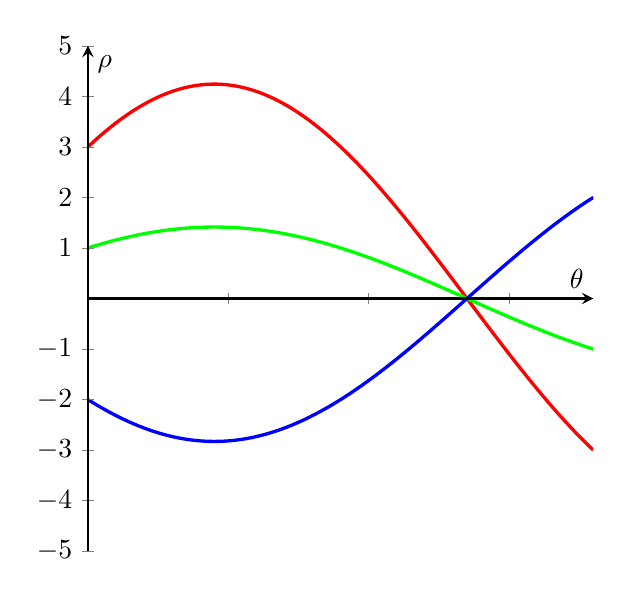
\begin{tikzpicture}
                        \begin{axis}[
                            axis on top=true,
                            axis line style=thick,
                            domain=0:180, samples=90,
                            axis lines=middle, xlabel=$\theta$, ylabel=$\rho$,
                            height=8cm, width=8cm,
                            enlargelimits=false,
                            xticklabels={,,},
                            ytick={-5,-4,...,5},
                            xmin=0, xmax=180,
                            ymin=-5, ymax=5
                        ]
                            \addplot[very thick, red] {3 * cos(\x) + 3 * sin(\x)};
                            \addplot[very thick, green] {cos(\x) + sin(\x)};
                            \addplot[very thick, blue] {-2 * cos(\x) - 2 * sin(\x)};
                        \end{axis}
                    \end{tikzpicture}
                \end{center}
                This gives the resultant vote $\theta = \frac{3\pi}{4}$ and $\rho = 0$.
                \medskip

                To perform this algorithm, we do the following;
                \begin{enumerate}[1.]
                    \itemsep0em
                    \item initialise the bins $H(\rho, \theta)$ to zero in the parameter space
                    \item for each edge point $(x, y)$;
                        \begin{enumerate}[a.]
                            \itemsep0em
                            \item for $\theta$ from $0$ to $\pi$
                                \begin{enumerate}[i.]
                                    \itemsep0em
                                    \item calculate $\rho = x\cos \theta + y\sin \theta$
                                    \item accumulate $H(\rho, \theta) = H(\rho, \theta) + 1$
                                \end{enumerate}
                        \end{enumerate}
                    \item find $(\rho, \theta)$ where $H(\rho, \theta)$ is a local maximum and larger than a threshold
                        \smallskip

                        This is done in a similar way to the previous lecture.
                        The local maximum allows multiple solutions to be detected, and the threshold reduces false positives.
                    \item the detected lines are given by $\rho = x\cos \theta + y\sin \theta$
                \end{enumerate}
                In contrast to model fitting (minimisation), Hough transform can simultaneously detect multiple lines (as long as they are local maximums and above a threshold) whereas the former can only detect a single line.
                Hough transform is robust to noise for two reasons.
                First, the initial edge map is generated after image smoothing (already suppressing noise).
                Furthermore, the broken edge maps are still able to vote and contribute to line detection.
                Similarly, it is also robust to object occlusion (objects overlapping, such as a tree obstructing part of a face).
                \medskip

                However, the computational complexity is high; we have to vote in a 2D or 3D parameter space for each edge point.
                We also need to set parameters carefully, such as parameters for the edge detector, the threshold for the accumulator, or the radius range (in the case of circles).
                \medskip

                This can be generalised to other shapes (which can be analytically represented), such as ellipses or planes in a 3D space.
                We can also weigh the votes, by taking the gradient magnitude (such that stronger edge points are weighted higher).
                \medskip

                In general, if it is a simple shape (such that there is no analytical equation), we can still vote as long as we have a model.
                For example, consider the case of pedestrian detection; we can vote for points above a patch where a foot is detected, and below where a head is detected.
            \subsubsection*{Circles}
                We can parameterise a circle as;
                $$(x - a)^2 + (y - b)^2 = r^2$$
                However, this is a very large parameter space (hence many bins).
                If we have some prior knowledge (such as the radius $r$), we can make the problem easier by reducing the search space - we can just vote for $a, b$ (the centre of the circle).
                The votes are still circles in the parameter space $H(a, b)$ (assuming $r = 1$);
                $$(a - x)^2 + (b - y)^2 = 1$$
                This can be seen graphically as the following (image space on the left, parameter space ($(a - x)^2 + (b - y)^2 = 1$) on the right);
                \begin{center}
                    \hfill
                    \begin{tikzpicture}
                        \begin{axis}[
                            axis on top=true,
                            axis line style=thick,
                            domain=-4:4, samples=9,
                            axis lines=middle, xlabel=$x$, ylabel=$y$,
                            height=8cm, width=8cm,
                            enlargelimits=false,
                            xtick={-4,-3,...,4},
                            ytick={-4,-3,...,4},
                            xmin=-4, xmax=4,
                            ymin=-4, ymax=4
                        ]
                            \node[circle, fill=red, inner sep=2pt] at (axis cs:3,2) {};
                            \node[circle, fill=green, inner sep=2pt] at (axis cs:2,1) {};
                            \node[circle, fill=blue, inner sep=2pt] at (axis cs:1,2) {};
                        \end{axis}
                    \end{tikzpicture}
                    \hfill
                    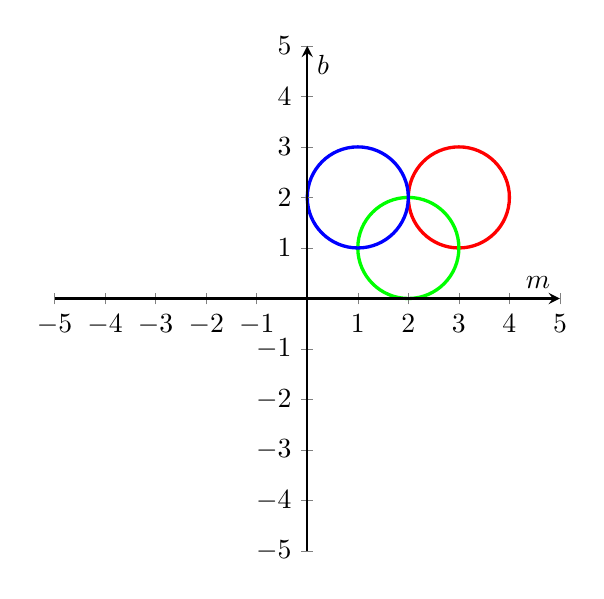
\begin{tikzpicture}
                        \begin{axis}[
                            axis on top=true,
                            axis line style=thick,
                            domain=-4:4, samples=9,
                            axis equal image,
                            axis lines=middle, xlabel=$m$, ylabel=$b$,
                            height=8cm, width=8cm,
                            enlargelimits=false,
                            xtick={-5,-4,...,5},
                            ytick={-5,-4,...,5},
                            xmin=-5, xmax=5,
                            ymin=-5, ymax=5
                        ]
                            \path (axis cs:0,0) coordinate (O);
                            \path (axis cs:1,0) coordinate (U);
                            \draw[very thick, red] let \p1=(O), \p2=(U), \n1={veclen(\x2-\x1,\y2-\y1)} in (axis cs:3,2) circle [radius=\n1];
                            \draw[very thick, green] let \p1=(O), \p2=(U), \n1={veclen(\x2-\x1,\y2-\y1)} in (axis cs:2,1) circle [radius=\n1];
                            \draw[very thick, blue] let \p1=(O), \p2=(U), \n1={veclen(\x2-\x1,\y2-\y1)} in (axis cs:1,2) circle [radius=\n1];
                        \end{axis}
                    \end{tikzpicture}
                    \hfill \phantom{}
                \end{center}
                If we don't know the radius, we set a range $r \in [r_\text{min}, r_\text{max}]$, and then perform a similar algorithm to before.
                \medskip

                Another representation of a circle can be done with trigonometric functions (parametric form);
                \begin{align*}
                    x & = a + r \cos \theta \\
                    y & = b + r \sin \theta
                \end{align*}
                However, if we know $\theta$, we can vote along a direction.
                Since we know the direction of an edge point (obtained from edge detection), we can narrow it down (along the gradient or opposite the gradient).
                We assume an accuracy of $\pm \phi$, and vote within that area.
                \begin{center}
                    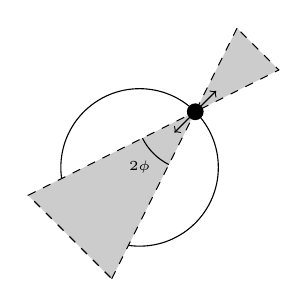
\begin{tikzpicture}
                        \draw (0, 0) circle (1);
                        \begin{scope}[shift={(0.707, 0.707)}, rotate={45}, scale={0.75}]
                            \draw[dashed, fill=black!20]
                            (1.5, 0.5) -- (0, 0) -- (1.5, -0.5) -- cycle
                            (-3, -1) -- (0, 0) -- (-3, 1) -- cycle;
                            \node[rbtb] at (0, 0) {};
                            \draw (0.5, 0) edge[<->] (-0.5, 0);
                            \draw (0, 0) ++(161.6:1) arc (161.6:198.4:1);
                        \end{scope}
                        \node at (0, 0) {\tiny $2 \phi$};
                    \end{tikzpicture}
                \end{center}
                The algorithm can be done as follows;
                \begin{enumerate}[1.]
                    \itemsep0em
                    \item initialise all bins $H(a, b, r)$ to zero
                    \item for each possible radius $r \in [r_\text{min}, r_\text{max}]$
                        \begin{enumerate}[a.]
                            \itemsep0em
                            \item for each edge point $(x, y)$;
                                \begin{enumerate}[i.]
                                    \itemsep0em
                                    \item let $\theta$ be gradient direction / opposite gradient direction
                                    \item calculate $a = x - r\cos \theta$ and $b = y - r\sin \theta$
                                    \item accumulate $H(a, b, r) = H(a, b, r) + 1$
                                \end{enumerate}
                        \end{enumerate}
                    \item find $(a, b, r)$ where $H(a, b, r)$ is a local maximum and larger than a threshold
                \end{enumerate}
        \subsection*{Lecture 8 - Interest Point Detection I}
            An interest point is a point we are interested in, and are useful for subsequent processing and analysis (classification, matching, retrieval, etc).
            These are commonly corners or blobs, where local image structure is rich.
            These are also known as keypoints, landmarks, or low-level features.
            \subsubsection*{Applications}
                We can define landmarks, on a face, which are most representative.
                Once we detect these landmarks, the locations can be used for purposes such as mood analysis, AR, etc.
                \medskip

                Another application is \textbf{image matching}; detecting relationships between images (such as orientation) and finding spatial correspondence between two images.
                This can be done by pixels (by using all information), by edges (using some information), or by interest points (using only important information).
                Matching with pixels often works by optimising a similarity metric (based on all pixels), with a spatial transformation $T$;
                $$\max_T \text{Similarity}(I_A, I_B(T))$$
                A more efficient approach is to find interest points and see how they are transformed between images (consider different perspectives of an art piece).
            \subsubsection*{Harris Detector}
                Corners are intersection of edges (which are high magnitude of gradient).
                For corner detection, by just looking at the gradient magnitude of a single pixel, we can't tell if it is a corner or edge pixel.
                However, if we look at the small windows, we can tell a difference;
                \begin{itemize}
                    \itemsep0em
                    \item flat \hfill change of intensity in \textbf{neither} direction
                    \item edge \hfill change of intensity along just \textbf{one} direction
                    \item corner \hfill change of intensity along \textbf{both} directions
                \end{itemize}
                We want to define a window $W$ and a window function $w$ (1 if it is in the window, 0 otherwise), where we have the \violet{sum of squared difference}, \teal{intensity in the shifted window} and the \blue{original intensity};
                $$\violet{E(u, v)} = \summation{(x, y) \in W}{} w(x, y)[\teal{(I(x + u, y + v)} - \blue{I(x, y)}]^2$$
                Note that the window function $w(x, y)$ is used as it isn't necessarily 1 inside, and 0 outside, we can use also use a Gaussian to put more focus on the middle of the window.
                \medskip

                We can use the following Taylor expansion (note that $I_x$ and $I_y$ denote the image derivative along $x$ and $y$ respectively);
                $$\teal{I(x + u, y + v)} = \blue{I(x, y)} + \red{uI_x(x, y) + vI_y(x, y)} + \dots$$
                Using just the first order approximation;
                \begin{align*}
                    E(u, v) & = \summation{}{} w(x, y)[\teal{I(x + u, y + v)} - \blue{I(x, y)}]^2 \\
                    & \approx \summation{}{} w(x, y)[\red{u\underbrace{I_x(x, y)}_{I_x} + v\underbrace{I_y(x, y)}_{I_y}}])^2 \\
                    & = \summation{}{} w(x, y)(u^2I_x^2 + 2uvI_xI_y + v^2I_y^2) \\
                    & = \summation{}{} w(x, y) \begin{bmatrix}
                        u & v
                    \end{bmatrix} \begin{bmatrix}
                        I_x^2 I_xI_y \\
                        I_xI_y & I_y^2
                    \end{bmatrix} \begin{bmatrix}
                        u \\ v
                    \end{bmatrix} & \text{written as matrix formula} \\
                    & = \begin{bmatrix}
                        u & v
                    \end{bmatrix} \summation{}{} w(x, y) \begin{bmatrix}
                        I_x^2 & I_xI_y \\
                        I_xI_y & I_y^2
                    \end{bmatrix} \begin{bmatrix}
                        u \\ v
                    \end{bmatrix}
                \end{align*}
                Therefore, for a small shift $(u, v)$, we have the approximation (note that $E(u, v)$ will be large when image derivatives are large);
                $$E(u, v) \approx \begin{bmatrix}
                    u & v
                \end{bmatrix} \mat{M} \begin{bmatrix}
                    u \\ v
                \end{bmatrix}$$
                Where $\mat{M} \in \mathbb{R}^{2 \times 2}$ is computed from the window function and image derivatives (this matrix will also provide the direction of changes);
                $$\mat{M} = \summation{x, y}{} w(x, y) \begin{bmatrix}
                    I_x^2 & I_xI_y \\
                    I_xI_y & I_y^2
                \end{bmatrix}$$
                We have the following simple cases (and examples) - note that these are \textbf{only} diagonals;
                \begin{itemize}
                    \itemsep0em
                    \item \textbf{flat region} \hfill small values on diagonal
                        $$\mat{M} = \begin{bmatrix}
                            0 & 0 \\
                            0 & 0
                        \end{bmatrix}$$
                    \item \textbf{edge} \hfill diagonal, large on one of diagonal
                        $$\mat{M} = \begin{bmatrix}
                            10 & 0 \\
                            0 & 0.1
                        \end{bmatrix}$$
                        In this case, we have a large change if shifting along $u$, but a small change if we shift along $v$, hence we have an edge.
                    \item \textbf{corner} \hfill diagonal, large on both diagonal
                        $$\mat{M} = \begin{bmatrix}
                            10 & 0 \\
                            0 & 10
                        \end{bmatrix}$$
                        If we move along either direction, there will be a large change, hence it is a corner.
                \end{itemize}
                However, in the case that $\mat{M}$ is more complex (such that it isn't a diagonal matrix), we can simplify it by performing eigen decomposition.
                Because $\mat{M}$ is a real symmetric matrix, we can decompose it as;
                $$\mat{M} = \mat{P} \mat{\Lambda} \mat{P}^\top$$
                In the above, $\mat{P}$ has eigenvectors (orthogonal to each other) as columns (and therefore $\mat{P}^\top$ has eigenvectors as rows), and $\mat{\Lambda}$ is a diagonal matrix with eigenvalues;
                $$\mat{\Lambda} = \begin{bmatrix}
                    \lambda_1 & 0 \\
                    0 & \lambda_2
                \end{bmatrix}$$
                Referring back to $E(u, v)$, we have the following;
                $$E(u, v) \approx \begin{bmatrix}
                    u & v
                \end{bmatrix} \mat{P} \mat{\Lambda} \mat{P}^\top \begin{bmatrix}
                    u \\ v
                \end{bmatrix}$$
                The same rules as above apply; however instead of moving along $u$, we instead move along the first eigenvector (and instead of moving along $v$, we move along the second eigenvector).
                The edges are no longer horizontal or vertical, they are in the directions of the eigenvectors.
                The eigenvalues can be interpreted as follows;
                \begin{center}
                    \begin{tikzpicture}[x=1.5cm, y=1.5cm]
                        \draw (0, 0) edge[->] (2, 0);
                        \draw (0, 0) edge[->] (0, 2);
                        \node at (2, -0.5) {$\lambda_1$};
                        \node at (-0.5, 2) {$\lambda_2$};
                        \begin{scope}[shift={(0.25, 1.75)}, scale={0.25}]
                            \draw (-0.5, 0) -- (-0.5, 0.5) -- (0.5, 0.5) -- (0.5, 0);
                            \draw[fill=black] (-0.5, 0) -- (0.5, 0) -- (0.5, -0.5) -- (-0.5, -0.5) -- cycle;
                        \end{scope}
                        \begin{scope}[shift={(0.25, 0.25)}, scale={0.25}]
                            \draw (-0.5, -0.5) -- (-0.5, 0.5) -- (0.5, 0.5) -- (0.5, -0.5) -- cycle;
                        \end{scope}
                        \begin{scope}[shift={(1.75, 0.25)}, rotate={90}, scale={0.25}]
                            \draw (-0.5, 0) -- (-0.5, 0.5) -- (0.5, 0.5) -- (0.5, 0);
                            \draw[fill=black] (-0.5, 0) -- (0.5, 0) -- (0.5, -0.5) -- (-0.5, -0.5) -- cycle;
                        \end{scope}
                        \begin{scope}[shift={(1.75, 1.75)}, scale={0.25}]
                            \draw (-0.5, 0) -- (-0.5, 0.5) -- (0.5, 0.5) -- (0.5, -0.5) -- (0, -0.5);
                            \draw[fill=black] (-0.5, -0.5) -- (-0.5, 0) -- (0, 0) -- (0, -0.5) -- cycle;
                        \end{scope}
                    \end{tikzpicture}
                \end{center}
                Here we have the following cases;
                \begin{itemize}
                    \itemsep0em
                    \item $\lambda_1 \sim 0$ and $\lambda_2 \sim 0$ \hfill flat
                    \item $\lambda_1 >> \lambda_2$ \hfill vertical edge
                    \item $\lambda_2 >> \lambda_1$ \hfill horizontal edge
                    \item $\lambda_1$ and $\lambda_2$ both large \hfill corner
                \end{itemize}
                However, we want to define a single number for `cornerness' (high when both eigenvalues are large).
                This can be defined in multiple ways;
                \begin{itemize}
                    \itemsep0em
                    \item \textit{Harris and Stephens (1988)}
                        $$R = \lambda_1\lambda_2 - k(\lambda_1 + \lambda_2)^2$$
                        Here $k$ is a small number, such as $0.05$.
                        The small $k$ ensures that the number does not become too small (when subtracted) when both eigenvalues are large.
                    \item \textit{Kanade and Tomasi (1994)}
                        $$R = \min(\lambda_1, \lambda_2)$$
                    \item \textit{Noble (1998)}
                        $$R = \frac{\lambda_1\lambda_2}{\lambda_1 + \lambda_2 + \epsilon}$$
                \end{itemize}
                However; notice that we only want the values of $\lambda_1\lambda_2$  and $\lambda_1 + \lambda_2$, therefore we do not need to perform eigen decomposition.
                Using the following properties for matrix determinant and trace, we can obtain the following;
                \begin{align*}
                    \det(\mat{M}) & = \det(\mat{P}\mat{\Lambda}\mat{P}^\top) \\
                    & = \det(\mat{\Lambda}) \\
                    & = \lambda_1 \lambda_2 \\
                    \mathrm{trace}(\mat{M}) & = \mathrm{trace}(\mat{P}\mat{\Lambda}\mat{P}^\top) \\
                    & = \mathrm{trace}(\mat{\Lambda}) \\
                    & = \lambda_1 + \lambda_2
                \end{align*}
                Therefore, we only need the determinant and trace for the original matrix to calculate $R$;
                $$R = \det(\mat{M}) - k(\mathrm{trace}(\mat{M}))^2$$
                This detector can also find strong responses at blobs and textures, as well as corners.
                The algorithm is as follows;
                \begin{enumerate}[1.]
                    \itemsep0em
                    \item compute $x$ and $y$ derivatives of an image \hfill $G$ can be the Sobel filter
                        \begin{align*}
                            I_x & = G_x * I \\
                            I_y & = G_y * I
                        \end{align*}
                    \item compute the matrix $\mat{M}$ at each pixel
                        $$\mat{M} = \summation{x, y}{} w(x, y) \begin{bmatrix}
                            I_x^2 & I_xI_y \\
                            I_xI_y & I_y^2
                        \end{bmatrix}$$
                    \item calculate the detector response
                        $$R = \lambda_1\lambda_2 - k(\lambda_1 + \lambda_2)^2$$
                    \item detect interest points which are local maxima (and $R$ above a certain threshold)
                \end{enumerate}
                Note that the Harris detector is \textbf{rotation-invariant}.
                We will still get the same change of intensities when shifting along a rotated direction - the eigenvalues of $\mat{M}$ remain the same, but the eigenvectors will change.
                However, it is not invariant to scale.
                At a different zooming scale, an edge may be detected as a corner or vice versa (for example if the circle arc is large it will be detected as an edge, but if it is small, it will be detected as a corner).
        \subsection*{Lecture 9 - Interest Point Detection II}
            \subsubsection*{Scale}
                The intuitive ideal for scaling is to check whether the Harris detector gives the highest response at a given scale.
                If the region looks most like a corner at scale $\sigma$, there should be a high response.
                $$\mat{M} = \summation{x, y}{} w(x, y) \begin{bmatrix}
                    I_x^2(\sigma) & I_x(\sigma)I_y(\sigma) \\
                    I_x(\sigma)I_y(\sigma) & I_y^2(\sigma)
                \end{bmatrix}$$
                The response is  determined by the eigenvalues of $\mat{M}$, which are determined by the derivatives $I_x(\sigma)$ and $I_y(\sigma)$.
                These are inversely proportional to scale $\sigma$; the larger the scale, the smaller the derivative magnitude.
                \medskip

                Consider signals which only differ by scale $s$ (and have same peak magnitude);
                $$f(x) = g(sx)$$
                However, when we look at the derivatives of the function, we have a different peak magnitude; since the derivative looks at how quickly the functions change.
                Since we have the relation above, we have;
                $$\blue{f(x + \Delta x)} - f(x) = \violet{g(sx + s \Delta x)} - g(sx)$$
                Looking at the Taylor expansion for the above, we have;
                \begin{align*}
                    f(x + \Delta x) & = \blue{f(x) + \Delta x \cdot f^\prime(x) + \dots} \\
                    g(x + \Delta x) & = g(x) + \Delta x \cdot g^\prime(x) + \dots \\
                    g(sx + s \Delta x) & = \violet{g(sx) + s\Delta x \cdot g^\prime(sx) + \dots} \\
                    \intertext{Substituting back into the first equation, it gives us the following}
                    \Delta x \cdot f^\prime(x) & = s \Delta x \cdot g^\prime(sx) \\
                    f^\prime & = sg^\prime(sx)
                \end{align*}
                This gives us the following result;
                $$\dif{f}{x} = s \cdot \dif{g}{x}\ \vline\ _{sx}$$
                Therefore, we can multiply derivative by its scale $s$ to allow for magnitude comparison across scales, with the scale adapted Harris detector;
                $$\mat{M} = \summation{x, y}{} w(x, y) \sigma^2 \begin{bmatrix}
                    I_x^2(\sigma) & I_x(\sigma)I_y(\sigma) \\
                    I_x(\sigma)I_y(\sigma) & I_y^2(\sigma)
                \end{bmatrix}$$
                We can apply the scale adapted detector at multiple scales - at each pixel we determine the scale with the largest response (at this scale, the region looks most like a corner).
                Something is detected as an interest point if it is a local maximum both along the scale dimension (most appropriate scale) and across space, therefore we can use $(x, y, \sigma)$ for the interest point.
                This gives the following adapted algorithm;
                \begin{enumerate}[1.]
                    \itemsep0em
                    \item for each scale $\sigma$
                        \begin{enumerate}[a.]
                            \itemsep0em
                            \item perform Gaussian smoothing with $\sigma$
                            \item calculate $x$ and $y$ derivatives of the smoothed image $I_x(\sigma)$ and $I_y(\sigma)$, respectively
                            \item at each pixel, compute the matrix $\mat{M}$ (see above)
                            \item calculate the detector response $R = \lambda_1 \lambda_2 - k(\lambda_1 + \lambda_2)^2$
                        \end{enumerate}
                    \item detect interest points which are local maxima across both scale and space, with $R$ above a threshold
                \end{enumerate}
            \subsubsection*{Laplacian of Gaussian (LoG)}
                This first performs Gaussian smoothing, followed by the Laplacian operator.
                The Laplacian is the sum of second derivatives, for a 2D image;
                $$\Delta f = \nabla^2 = \pdif{^2f}{x^2} + \pdif{^2f}{y^2}$$
                We have the following filter;
                $$\underbrace{\begin{bmatrix}
                    \textcolor{black!33}{0} & \textcolor{black!33}{0} & \textcolor{black!33}{0} \\
                    1 & -2 & 1 \\
                    \textcolor{black!33}{0} & \textcolor{black!33}{0} & \textcolor{black!33}{0}
                \end{bmatrix}}_{\pdif{^2f}{x^2}} + \underbrace{\begin{bmatrix}
                    \textcolor{black!33}{0} & 1 & \textcolor{black!33}{0} \\
                    \textcolor{black!33}{0} & -2 & \textcolor{black!33}{0} \\
                    \textcolor{black!33}{0} & 1 & \textcolor{black!33}{0}
                \end{bmatrix}}_{\pdif{^2f}{y^2}} = \underbrace{\begin{bmatrix}
                    0 & 1 & 0 \\
                    1 & -4 & 1 \\
                    0 & 1 & 0
                \end{bmatrix}}_{\text{Laplacian filter}}$$
                The second derivative is even more sensitive to noise than the first derivative.
                \medskip

                The Laplacian of Gaussian filter is as follows (where $h$ is the Gaussian kernel);
                $$\Delta(f * h) = \pdif{^2(f * h)}{x^2} + \pdif{^2(f * h)}{y^2} = f * \left(\pdif{^2h}{x^2} + \pdif{^2h}{y^2}\right)$$
                Since we know the formation of a 2D Gaussian, we can derive the following;
                $$\pdif{^2h}{x^2} + \pdif{^2h}{y^2} = -\frac{1}{\pi\sigma^4}\left(1 - \frac{x^2 + y^2}{2\sigma^2}\right)e^{-\frac{x^2 + y^2}{2\sigma^2}}$$
                LoG can also be a good interest point detector.
                We need to ensure it is comparable between scales (note that $I_{xx}$ denotes the second derivative, we need to multiply by $\sigma^2$ rather than just $\sigma$; without the multiplication we have the LoG response at scale $\sigma$);
                $$\mathrm{LoG}_\text{norm}(x, y, \sigma) = \sigma^2\left(I_{xx}(x, y, \sigma) + I_{yy}(x, y, \sigma)\right)$$
            \subsubsection*{Difference of Gaussian (DoG)}
                This is defined as; the difference of Gaussians with different scales (note that $I$ is the image, Lowe suggests $k = \sqrt{2}$);
                $$\mathrm{DoG}(x, y, \sigma) = I * G(k \sigma) - I * G(\sigma)$$
                This approximates the normalised Laplacian of Gaussian, which provides convenience in calculating the response across different scales;
                $$\mathrm{DoG}(x, y, \sigma) \approx (k - 1) \sigma^2 \nabla^2 G(x, y, \sigma)$$
                DoG filters are used in SIFT, which is a pipeline for detecting and describing interest points.
            \subsubsection*{Interest Point Detectors}
                All of the interest point detectors are scale-invariant (other than the Harris detector, before normalisation);
                \begin{center}
                    \begin{tabular}{ll}
                        detector & response \\
                        \hline
                        scale adapted Harris detector & $\lambda_1\lambda_2 - k(\lambda_1 + \lambda_2)^2$ \\
                        normalised Laplacian of Gaussian & $\sigma^2\left(I_{xx}(x, y, \sigma) + I_{yy}(x, y, \sigma)\right)$ \\
                        difference of Gaussian & $I * G(k \sigma) - I * G(\sigma)$
                    \end{tabular}
                \end{center}
                All of these follow similar procedures, where we calculate the detector responses across values, providing a three-dimensional response map ($x$ and $y$, as well as $\sigma$ for scale).
                From here, we find local extrema across both space and scale.
        \subsection*{Lecture 10 - Feature Description I}
            \subsubsection*{Pixel Intensity}
                A simple method for describing a feature is o use the intensity of a pixel.
                However, this is sensitive to absolute value (the intensity of the same point will change during different lighting conditions).
                This descriptor is not discriminative; many pixels can have the same intensity within an image.
                Furthermore, a single pixel cannot represent any local content (such as an edge, or an object).
            \subsubsection*{Patch Intensities}
                This improves on a single pixel, as we can take some window representing the local pattern.
                If the images are of similar intensity range, and are roughly aligned, it can perform well.
                However, it will still be sensitive to absolute intensity values as before.
                Furthermore, it is not rotation-invariant; for example if we look at an image from a different rotation we can still tell what the image is.
            \subsubsection*{Gradient Orientation}
                While gradient magnitude is sensitive to intensity changes, orientation isn't.
                However, this still isn't rotation-invariant.
            \subsubsection*{Histogram}
                We can take the intensity histogram of a patch.
                This is done by binning the intensity values of a patch, and generating a histogram from these values.
                This has several benefits, where it is robust to rotation, as well as being robust to scaling (if the entire image is enlarged).
                However, it is still sensitive to intensity changes.
                \medskip

                As such, we can consider combining the advantages of gradient orientation and the advantages of this histogram.
            \subsubsection*{SIFT (Scale-invariant Feature Transform)}
                This is an algorithm for detecting and describing local features.
                It transforms an intensity image to a set of interest points, each of which is described by a feature vector.
                \begin{enumerate}[1.]
                    \itemsep0em
                    \item detection of scale-space extrema
                        \smallskip

                        The first step is to search across scales and pixel locations, looking for interest points.
                        This uses the difference of Gaussian filter, as previously encountered (in the SIFT paper, the different scales are multiplied by $\sqrt{2}$ continuously; $\sigma, \sqrt{2}\sigma, 2\sigma, 2\sqrt{2}\sigma, 4\sigma, \dots$);
                        $$\mathrm{DoG}(x, y, \sigma) = I * G(k \sigma) - I * G(\sigma)$$
                        As before, a point is an interest point if it is a local extremum both along the scale dimension (most appropriate scale) and across space.
                        \medskip

                        Note that extrema means both minima and maxima.
                        If the input interest point is a very bright blob, DoG filter gives a negative response, and vice versa (a dark blob will lead to a positive response).
                    \item keypoint localisation
                        \smallskip

                        The initial version of SIFT simply locates the keypoints at the scale-space extrema (which we have from above).
                        An improved version fits a model onto nearby data, improving accuracy for image matching.
                        \medskip

                        A quadratic function can be \textcolor{blue!50!black}{fitted} onto the DoG response of neighbouring pixels, and the location and scale of extremum for this (quadratic) function can be estimated.
                        \begin{center}
                            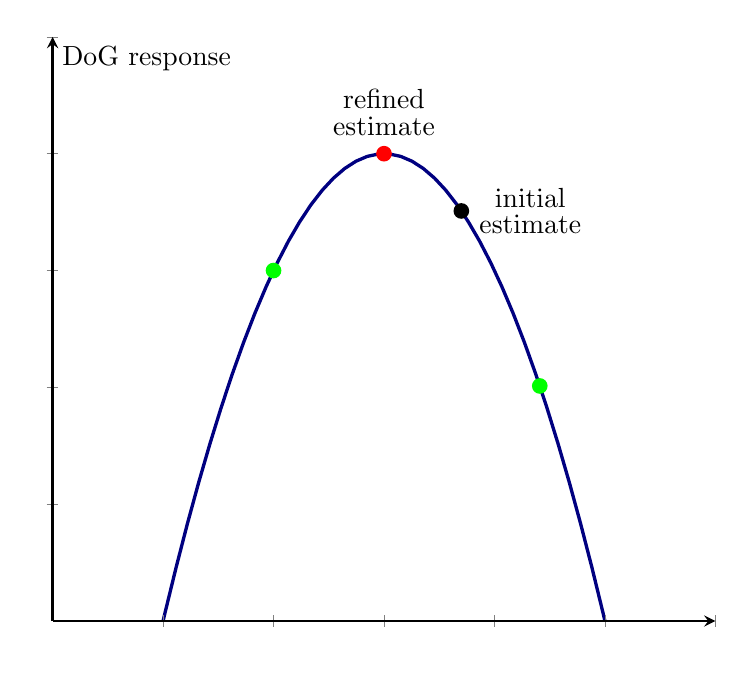
\begin{tikzpicture}
                                \begin{axis}[
                                    axis on top=true,
                                    axis line style=thick,
                                    domain=0:6, samples=60,
                                    axis lines=middle, xlabel=, ylabel=DoG response,
                                    height=9cm, width=10cm,
                                    enlargelimits=false,
                                    xticklabels={,,},
                                    yticklabels={,,},
                                    xmin=0, xmax=6,
                                    ymin=0, ymax=5
                                ]
                                    \addplot[blue!50!black, very thick] {4 - (\x - 3)^2};
                                    \node[label={90:{\shortstack{refined\\estimate}}}, circle, fill=red, inner sep=2pt] at (axis cs:3,4) {};
                                    \node[label={0:{\shortstack{initial\\estimate}}}, circle, fill=black, inner sep=2pt] at (axis cs:3.7,3.51) {};
                                    \node[circle, fill=green, inner sep=2pt] at (axis cs:2,3) {};
                                    \node[circle, fill=green, inner sep=2pt] at (axis cs:4.41,2.012) {};
                                \end{axis}
                            \end{tikzpicture}
                        \end{center}
                        Denote the DoG response as $D(x, y, \sigma)$ or $D(\vec{x})$, where $\vec{x} = (x, y, \sigma)^\top$ (containing both location and scale).
                        By Taylor expansion we have (omitting higher order terms);
                        $$D(\vec{x} + \Delta\vec{x}) = D(\vec{x}) + {\underbrace{\pdif{D}{\vec{x}}}_\text{(1)}}^\top \Delta\vec{x} + \frac{1}{2}\Delta\vec{x}^\top \underbrace{\pdif{^2D}{\vec{x}^2}}_\text{(2)} \Delta\vec{x}$$
                        \begin{enumerate}[(1)]
                            \itemsep0em
                            \item first derivatives can be estimated with finite difference
                                $$\pdif{D}{\vec{x}} = \frac{D(x + 1, y, \sigma) - D(x - 1, y, \sigma)}{2}$$
                            \item second derivatives / Hessian can also be estimated with finite difference
                        \end{enumerate}
                        This gives us a quadratic function for $\Delta\vec{x}$, the shift to the refined estimate, from the initial estimate $\vec{x}$.
                        Therefore, to find a refined extrema for the function;
                        $$\pdif{D(\vec{x} + \Delta\vec{x})}{\Delta\vec{x}} = \pdif{D}{\vec{x}} + \pdif{^2D}{\vec{x}^2}\Delta\vec{x} = 0 \Rightarrow \Delta \vec{x} = -\pdif{^2D}{\vec{x}^2}^{-1} \pdif{D}{\vec{x}}$$
                        Shifting the initial estimate by $\Delta\vec{x}$ gives us the \red{refined estimate}.
                        \medskip

                        Recall that $\vec{x}$ is a 3D vector, and gives both location and scale.
                        This means that we can get refined estimates for the location (sub-pixel accuracy), as well as a refined scale, which gives values between the scales of $\sigma, \sqrt{2}\sigma, 2\sigma, 2\sqrt{2}\sigma, 4\sigma, \dots$
                    \item orientation assignment
                        \smallskip

                        This step attempts to assign a consistent orientation to each keypoint, based on image properties.
                        Feature descriptors can then be represented relative to this orientation, to achieve rotation-invariance.
                        To do this, we need to know the orientation of the feature, and once we have this, we can perform sampling in a rotated coordinate system when we calculate features, giving us the same features.
                        \medskip

                        We can calculate the gradient orientation for pixels in some neighbourhood and vote for the dominant orientation.
                        We can create an orientation histogram with 36 bins ($10^\circ$ per bin), and each pixel in the neighbourhood votes for an orientation bin (weighted by the gradient magnitude) - the keypoint will be assigned an orientation, which would be the majority bin.
                        \medskip

                        We now have the location $(x, y)$, scale $\sigma$, and dominant orientation $\theta$.
                        Using this, we an draw samples using a window size proportional to $\sigma$ rotated by $\theta$.
                    \item keypoint descriptor
                        \smallskip

                        Now that we have sample points, we need to describe the local image content.
                        SIFT uses a histogram of gradient orientations.
                        \medskip

                        A histogram of gradient orientations is made from the calculated gradient magnitudes and orientation for the sampling points.
                        These orientations are calculated relative to the dominant orientation $\theta$.
                        In practice, subregions are used, with each subregion having $4 \times 4$ samples - each subregion will have an orientation histogram, which (when combined) describes what it looks like around a given keypoint.
                        \medskip

                        For each subregion, we can construct an orientation histogram with 8 bins (each bin representing $45^\circ$).
                        This can also be represented as 8 arrows (seen below), where the length of the arrow denotes the sum of the gradient magnitude along a given direction;
                        \begin{center}
                            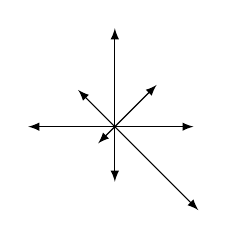
\begin{tikzpicture}
                                \begin{scope}[rotate={0}]
                                    \draw (0, 0) edge[-latex] (1, 0);
                                \end{scope}
                                \begin{scope}[rotate={45}]
                                    \draw (0, 0) edge[-latex] (0.75, 0);
                                \end{scope}
                                \begin{scope}[rotate={90}]
                                    \draw (0, 0) edge[-latex] (1.25, 0);
                                \end{scope}
                                \begin{scope}[rotate={135}]
                                    \draw (0, 0) edge[-latex] (0.66, 0);
                                \end{scope}
                                \begin{scope}[rotate={180}]
                                    \draw (0, 0) edge[-latex] (1.1, 0);
                                \end{scope}
                                \begin{scope}[rotate={225}]
                                    \draw (0, 0) edge[-latex] (0.3, 0);
                                \end{scope}
                                \begin{scope}[rotate={270}]
                                    \draw (0, 0) edge[-latex] (0.7, 0);
                                \end{scope}
                                \begin{scope}[rotate={315}]
                                    \draw (0, 0) edge[-latex] (1.5, 0);
                                \end{scope}
                            \end{tikzpicture}
                        \end{center}
                        In Lowe's implementation, 16 subregions were used.
                        This gives the descriptor a dimensionality of $128 = 16 \times 8$ (since each subregion has 8 bins); meaning each keypoint is described with a feature vector of 128 elements.
                        \medskip

                        This descriptor is robust to rotation due to a consideration of a dominant orientation, similarly it is robust to scaling as we draw samples from a window proportional to scale.
                        It is also robust to changes in illumination since we use gradient orientations for feature description.
                \end{enumerate}
            \subsubsection*{Keypoint Matching}
                Keypoints between two images are matched by identifying the nearest neighbours (which is defined by the Euclidean distance of SIFT descriptors).
                Each keypoint in image $A$ identifies its nearest neighbour in the database of keypoints for image $B$.
                However, we may not need to find the exact nearest neighbours for the sake of efficiency.
                \medskip

                Suppose we find a keypoint $(x, y)$ in $A$ that corresponds to a keypoint $(u, v)$ in $B$.
                We assume they are related with an affine transformation (\violet{rotation, scaling, etc.} and \teal{translation});
                $$\begin{bmatrix}
                    u \\ v
                \end{bmatrix} = \violet{\begin{bmatrix}
                    m_1 & m_2 \\
                    m_3 & m_4
                \end{bmatrix}} \begin{bmatrix}
                    x \\ y
                \end{bmatrix} + \teal{\begin{bmatrix}
                    t_x \\ t_y
                \end{bmatrix}}$$
                However, with many pairs of corresponding keypoints, we can write the equation as;
                $$\begin{matrix}
                    \text{keypoint 1} \\
                    \phantom{} \\
                    \text{keypoint 2} \\
                    \phantom{} \\
                    \phantom{}
                \end{matrix} \begin{bmatrix}
                    x_1 & y_1 & 0 & 0 & 1 & 0 \\
                    0 & 0 & x_1 & y_2 & 0 & 1 \\
                    x_2 & y_2 & 0 & 0 & 1 & 0 \\
                    0 & 0 & x_2 & y_2 & 0 & 1 \\
                    \vdots & \vdots & \vdots & \vdots & \vdots & \vdots
                \end{bmatrix} \begin{bmatrix}
                    m_1 \\ m_2 \\ m_3 \\ m_4 \\ t_x \\ t_y
                \end{bmatrix} = \begin{bmatrix}
                    u_1 \\ v_1 \\ u_2 \\ v_2 \\ \vdots
                \end{bmatrix}$$
                This can also be written as a linear system, where only $\vec{m}$ is unknown;
                $$\mat{A}\vec{m} = \vec{b}$$
                However, we can obtain the least-square solution to the linear system with the \violet{Moore-Penrose inverse}, minimising the squared difference $|| \mat{A}\vec{m} - \vec{b} ||^2$;
                $$\vec{m} = \violet{\left(\mat{A}^\top\mat{A}\right)^{-1}\mat{A}^\top} \vec{b}$$
                Once this is solved, we have the spatial transformation between the two images.
            \subsubsection*{RANSAC}
                However, the squared difference can be sensitive to outliers (noise) - in our case, this would be points that are deemed to be corresponding but actually aren't.
                To ensure our solution is robust to the outliers we can use methods which consider outliers in the model fitting such as \textbf{RANSAC (Random Sample Consensus)}.
                \medskip

                RANSAC aims to find the best fitting line to a given set of points.
                The algorithm to perform this is as follows (this is done repeatedly until we get a good fitting line);
                \begin{enumerate}[1.]
                    \itemsep0em
                    \item randomly sample some points (the example shows 2 points in a 2D illustration)
                    \item fit a line along the sampled points
                    \item find the number of \textbf{inliers} within a threshold to the line
                    \item terminate if enough inliers have been found, or we have reached a certain number of iterations
                \end{enumerate}
        \subsection*{Lecture 11 - Feature Description II}
            \subsubsection*{SIFT}
                As mentioned before, the SIFT descriptor at each interest point is formed by the concatenation of the gradient orientation histograms for 16 subregions (each having $128 = 16 \times 8$ values).
                Calculating magnitudes and orientations can be slow, especially if we want real-time performance (such as stitching on a phone camera, or for robotics).
                \medskip

                One solution is to implement SIFT on FPGAs, which is faster than a CPU (once configured to perform this function).
                Another approach is to improve the algorithm, where we decompose the pipeline into several steps, where we evaluate how to improve each step.
                The pipeline for image matching is as follows;
                \begin{enumerate}[1.]
                    \itemsep0em
                    \item \textbf{feature detection} (e.g. DoG)
                        \smallskip

                        There are a number of approaches for faster feature detection, including separable filtering, downsampling the image, or cropping the Gaussian kernel.
                    \item \textbf{feature description} (e.g. SIFT)
                        \smallskip

                        Here we can consider whether we can evaluate the gradient orientation faster, or if we can use a different method of describing the local content.
                    \item \textbf{interest point matching}
                        \smallskip

                        Here we can approximate the nearest neighbour search, as well as use a lower-dimensional feature vector.
                \end{enumerate}
            \subsubsection*{SURF (Speeded-Up Robust Features)}
                To accelerate computation, SURF only computes gradients along horizontal and vertical directions (rather than all of them) using \textbf{Haar wavelets}.
                Recall that the SIFT descriptor needs to calculate a histogram of gradient orientations, for each of the 16 subregions centred at an interest point.
                \medskip

                SURF still uses the same subregions and sample points, however we do not need to calculate gradients for arbitrary orientations.
                This applies two very simple filters (Haar wavelets, of size $2 \times 2$ or $4 \times 4$), $d_y$ and $d_x$ onto the sample points;
                \begin{center}
                    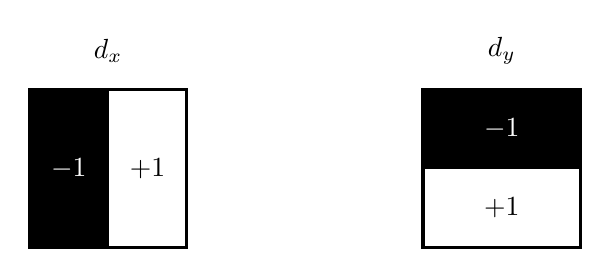
\begin{tikzpicture}
                        \begin{scope}
                            \node at (1, 0.5) {$d_x$};
                            \draw[very thick] (0, 0) -- (2, 0) -- (2, -2) -- (0, -2) -- cycle;
                            \draw[fill=black] (0, 0) -- (1, 0) -- (1, -2) -- (0, -2) -- cycle;
                            \node[white] at (0.5, -1) {$-1$};
                            \node at (1.5, -1) {$+1$};
                        \end{scope}
                        \begin{scope}[shift={(5, 0)}]
                            \node at (1, 0.5) {$d_y$};
                            \draw[very thick] (0, 0) -- (2, 0) -- (2, -2) -- (0, -2) -- cycle;
                            \draw[fill=black] (0, 0) -- (2, 0) -- (2, -1) -- (0, -1) -- cycle;
                            \node[white] at (1, -0.5) {$-1$};
                            \node at (1, -1.5) {$+1$};
                        \end{scope}
                    \end{tikzpicture}
                \end{center}
                Summing the pixel intensities with a weight of 1 or $-1$ is very fast, since it is either an addition or subtraction.
                For each subregion, we sum up the Haar wavelet responses over the sample points - the descriptor for a given subregion is defined by 4 elements (the sum of values and the sum of absolute values);
                $$\left(\summation{}{}d_x, \summation{}{}d_y, \summation{}{}|d_x|, \summation{}{}|d_y|\right)$$
                We can visualise the meanings of these descriptors as follows.
                If all four values are low, then the subregion is mostly homogeneous.
                If there are patterns similar to zebra stripes, a change from black to white, and then from white back to back would give a sum of 0 when we look at $d_x$ (since they cancel out).
                However, if we look at $|d_x|$, the value doubles (since they will not cancel).
                \begin{center}
                    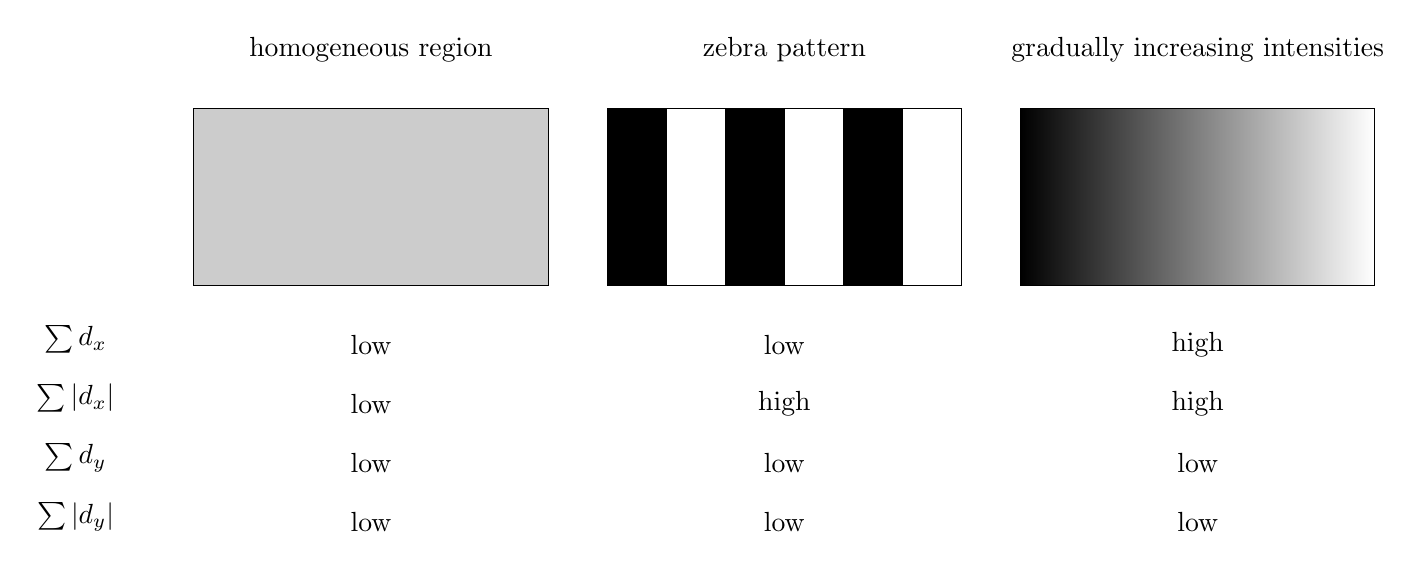
\begin{tikzpicture}[x=0.75cm, y=0.75cm]
                        \node at (-2, -4) {$\summation{}{}d_x$};
                        \node at (-2, -5) {$\summation{}{}|d_x|$};
                        \node at (-2, -6) {$\summation{}{}d_y$};
                        \node at (-2, -7) {$\summation{}{}|d_y|$};
                        \begin{scope}
                            \node at (3, 1) {homogeneous region};
                            \draw[fill=black!20] (0, 0) -- (6, 0) -- (6, -3) -- (0, -3) -- cycle;
                            \node at (3, -4) {low};
                            \node at (3, -5) {low};
                            \node at (3, -6) {low};
                            \node at (3, -7) {low};
                        \end{scope}
                        \begin{scope}[shift={(7, 0)}]
                            \node at (3, 1) {zebra pattern};
                            \draw (0, 0) -- (6, 0) -- (6, -3) -- (0, -3) -- cycle;
                            \draw[fill=black] (0, 0) -- (1, 0) -- (1, -3) -- (0, -3) -- cycle;
                            \draw[fill=black] (2, 0) -- (3, 0) -- (3, -3) -- (2, -3) -- cycle;
                            \draw[fill=black] (4, 0) -- (5, 0) -- (5, -3) -- (4, -3) -- cycle;
                            \node at (3, -4) {low};
                            \node at (3, -5) {high};
                            \node at (3, -6) {low};
                            \node at (3, -7) {low};
                        \end{scope}
                        \begin{scope}[shift={(14, 0)}]
                            \node at (3, 1) {gradually increasing intensities};
                            \draw[left color=black, right color=white] (0, 0) -- (6, 0) -- (6, -3) -- (0, -3) -- cycle;
                            \node at (3, -4) {high};
                            \node at (3, -5) {high};
                            \node at (3, -6) {low};
                            \node at (3, -7) {low};
                        \end{scope}
                    \end{tikzpicture}
                \end{center}
                The SURF descriptor still uses $16 = 4 \times 4$ subregions, each with 4 elements.
                This leads to a dimensionality of 64 for each interest point.
                Compared to SIFT, it is approximately 5 times faster due to the use of simple Haar wavelets.
                \medskip

                If we know the ground truth (in this case, the transformation between image $A$ and $B$), we can perform quantitative analysis on the performance of algorithms.
                The paper shows that SURF performs as well as SIFT in matching.
            \subsubsection*{BRIEF (Binary Robust Independent Elementary Features)}
                In both SIFT and SURF, each dimension is a floating-point number (represented in 4 bytes), and our comparison of feature vectors are done with Euclidean distance.
                Ideally, we'd want to make feature description and matching even faster.
                \medskip

                We can further shorten the descriptor by performing quantisation (converting a continuous number into a discrete number, hence 8 bits for the range $[0, 255]$), or even performing binarization (converting each into a binary number).
                \medskip

                Haar wavelets in SURF compare a local region toe another, giving a difference (which is a float).
                In BRIEF, comparing points $p, q$ will result in a binary value as an output (1 if $q$ is brighter than $p$);
                $$\tau(p, q) = \begin{cases}
                    1 & \text{if } I(p) < I(q) \\
                    0 & \text{otherwise}
                \end{cases}$$
                BRIEF randomly sample $n_d$ pairs of points for binary tests; this random pattern is only determined once, and the same pattern will be applied to all interest points.
                If we set $n_d = 256$, we will perform 256 tests in total, each giving us a single bit (with a total of 32 bytes; SIFT uses 128 bytes, and SURF uses 64 bytes).
                The descriptor is then a $n_d$-dimensional bitstring.
                \medskip

                Note that this is also fast to compute, as we can perform bit shifting (~<< n~ denotes a bit shift by ~n~ places).
                For example, if we performed 8 binary tests, we could do the following;
                \begin{lstlisting}
                    descriptor = ((I(p1) < I(q1)) << 7) + ((I(p2) < I(q2)) << 6)
                               + ((I(p3) < I(q3)) << 5) + ((I(p4) < I(q4)) << 4)
                               + ((I(p5) < I(q5)) << 3) + ((I(p6) < I(q6)) << 2)
                               + ((I(p7) < I(q7)) << 1) + ((I(p8) < I(q8)) << 0)
                \end{lstlisting}
                \medskip

                Not only does it use less memory, the computation only compares two numbers, without calculating gradient orientation like in SIFT, or the intensity difference like in SURF.
                We also avoid calculating the Euclidean distance, instead we use the Hamming distance.
                This allows for an efficient calculation by performing a bitwise XOR between two descriptors, and then taking a bit count - both of which can be done extremely quickly on modern CPUs in very few instructions.
                For example;
                \begin{center}
                    ~10001001 XOR 11000011 = 01001010~, thus a Hamming distance of 3
                \end{center}
                However; BRIEF isn't rotation-invariant nor scale-invariant.
                It assumes that the images taken are from a camera where the movement \textbf{only involves translation}.
                By combining all of the above, BRIEF is approximately 40 times faster than SURF, hence being around 200 times faster than SIFT.
                Furthermore, if there is no rotation or scaling, BRIEF is comparable to SURF in terms of matching accuracy.
            \subsubsection*{Image Similarity}
                Image similarity can be defined by the number of matched point.
                Intuitively, if two images are similar, there should be a higher number of interest points that can be matched together.
                See \textit{VisualRank}.
            \subsubsection*{HOG (Histograms of Oriented Gradient)}
                We can also extend the idea of feature descriptors (which describe local content centred at a point) to describe the feature of a large region, or even a whole image.
                \medskip

                While HOG and SIFT both use gradient orientation histograms for feature descriptions, HOG differs in that it describes features for a large image region (rather than a point).
                HOG divides a large region into a (dense) grid of cells, describes each cell, and concatenates the local descriptions to form a global description.
                \medskip

                In the example, we divide the image into equally spaced cells (each of $8 \times 8 pixels$).
                4 of these cells form a block; and we calculate the gradient orientation histogram for a block (thus forming a description of that block).
                Note that the description vector $\vec{v}$, which is the concatenation of the 4 histograms (from each cell), is normalised to form a locally normalised descriptor - note the inclusion of a small value $\epsilon$ to improve numerical stability.
                This is done to prevent issues between differing brightnesses;
                $$\vec{v_\text{norm}} = \frac{\vec{v}}{\sqrt{|| \vec{v} ||_2^2 + \epsilon^2}}$$
                The block is then shifted along horizontally by one cell (8 pixels in our case), note that there will be some overlap between the blocks.
                The HOG descriptor is then formed by concatenating all the normalised local descriptors for all blocks.
                \medskip

                We can use HOG to perform feature extraction from an input image to a feature representation.
                Feature extraction transforms an input image into low-dimensional vectors for easier comparison or matching.
                A classifier (trained with a dataset consisting of images, and often labels) can be used to give an output label to the feature representation.
        \subsection*{Lecture 12 - Image Classification I}
            This lecture starts with some motivation on image classification.
            The ImageNet project aims to collect $80,000$ classes, with each class having between $500$ to $1,000$ images.
            The ILSVRC uses a subset of this, with only $1,000$ (simpler) classes used; there are also no overlap between classes, since pairs of classes cannot be ancestors of each other.
            In ImageNet classes, all classes are organised as a tree.
            Below the root node, ImageNet has 12 subtrees (with each subtree expanding further into many classes);
            \begin{itemize}
                \itemsep0em
                \item mammal
                \item bird
                \item fish
                \item reptile
                \item amphibian
                \item vehicle
                \item furniture
                \item musical instrument
                \item geological formation
                \item tool
                \item flower
                \item fruit
            \end{itemize}
            These classes are defined with concepts from our natural language defined by WordNet (a lexical database of English).
            WordNet groups nouns into sets of cognitive synonyms (synsets), each expressing a \textbf{distinct} concept - these synsets will form the leaves of the tree, with the concepts already being organised as a tree.
            \subsubsection*{Classifier}
                This lecture is literally just going over stuff in \textbf{CO395}.
                For example, drawing a line as a classifier for data points in 2D space.
                When labels are not available for training data, we perform unsupervised learning; a common technique is to perform clustering for classification.
            \subsubsection*{MNIST Example}
                The example we go through will use the handwritten digit recognition dataset from MNIST - there are $60,000$ training samples and another $10,000$ reserved for testing.
                Each sample is a $28 \times 28$ image, which is labelled with a class from 0 to 9.
                \medskip

                However, we need to perform some pre-processing.
                We need to first find where the digit is in a large image, normalise the size of the digit to $28 \times 28$, as well as normalising the location (place the mass centre in the image centre).
                Sometimes slant correction may be performed, shifting each row to force the principal axis to become vertical.
                MNIST provides both datasets.
                \medskip

                There are two ways to extract features, either with hand-crafted techniques (such as HOG or pixel intensities), or learnt features such as CNNs.
                After which, we perform classification, with classifiers like KNN (once again, see \textbf{CO395}).
                \medskip

                To define the neighbours, we need a distance metric between two data points $\vec{x}$ and $\vec{y}$;
                \begin{itemize}
                    \itemsep0em
                    \item \textbf{Euclidean distance}
                        $$D(\vec{x}, \vec{y}) = \sqrt{(x_1 - y_1)^2 + \cdots + (x_n - y_n)^2}$$
                        In our case, we have $784 = 28 \times 28$ dimensions.
                        If each dimension has different scales, it can be better to normalise the feature vector (for example, weights and heights have different value ranges depending on the units).
                        An example is to normalise each dimension to a Gaussian distribution $\mathcal{N}(0, 1)$, allowing for the dimensions to be treated fairly.
                    \item \textbf{cosine distance}
                        $$D(\vec{x}, \vec{y}) = \frac{\vec{x} \cdot \vec{y}}{|| \vec{x} ||\ || \vec{y} ||} = \frac{x_1y_1 + \cdots + x_ny_n}{\sqrt{\summation{i = 1}{n}x_i^2}\sqrt{\summation{i = 1}{n}y_i^2}}$$
                    \item \textbf{generalised}
                        \smallskip

                        The Manhattan distance uses the $\ell_1$-norm;
                        $$D_1(\vec{x}, \vec{y}) = \summation{i = 1}{n}| x_i - y_i |$$
                        A more general form is the $\ell_p$-norm (note that the Euclidean distance is the $\ell_2$-norm);
                        $$D_p(\vec{x}, \vec{y}) = \left(\summation{i = 1}{n} | x_i - y_i |^p\right)^{\frac{1}{p}}$$
                \end{itemize}
                Using $K=1$, it can already work quite well.
                However, we may still have some inaccuracies, where a 7 may be classified as a 3, a 7 being classified as 0, or an 8 being classified as a 5, and so on.
                \medskip

                The lecture then goes over hyperparameter tuning for $K$, finding that $K=3$ is ideal for the MNIST dataset, with a $2.4\%$ error rate.
                KNN has no training step, is simple (but quite effective), and can also handle multi-class classification easily.
                However, it is expensive to use KNN in terms of both storage of training data and searching (for an extremely large set, the computational cost can become very expensive).
                \medskip

                Suppose we have $N$ training images, and $M$ test images.
                While we have no training time, the computational cost to classify all $M$ test images is $O(MN)$.
                \medskip

                However, we are typically fine with slow training (since we can perform the training on high-powered hardware), but we want the test time to be fast (since it may be deployed on weaker hardware).
            \subsubsection*{Features}
                For simple pre-processed images (like in our example), it might be fine to use the $28 \times 28$ pixel intensities as the feature vector.
                However, generally it may not be ideal to use pixel intensities, since it isn't invariant to scale nor rotation (and is generally a much higher dimension).
        \subsection*{Lecture 13 - Image Classification II}
            \subsubsection*{Linear Classifier}
                A linear classifier, in 2D, has the form;
                $$w_1x_1 + w_2x_2 + b = 0$$
                The rule of the classifier assigns a class $c$ on $x$ based on the following;
                $$c = \begin{cases}
                    1 & \text{if } w_1x_1 + w_2x_2 + b \geq 0 \\
                    -1 & \text{otherwise}
                \end{cases}$$
                For a linear classifier, once we know $\vec{w}$ and $b$, we can discard the training data (unlike in KNN).
                This is much faster in test time.
                \medskip

                For a more general case, the linear model is as follows (where we have the \violet{weights / normal}, \teal{data / feature}, and \blue{bias});
                $$\violet{\vec{w}} \cdot \teal{\vec{x}} + \blue{b} = 0$$
                Similarly, we have the same rule to assign class $c$;
                $$c = \begin{cases}
                    1 & \vec{w} \cdot \vec{x} + b \geq 0 \\
                    -1 & \text{otherwise}
                \end{cases}$$
            \subsubsection*{Linear SVM (Support Vector Machine)}
                To determine the maximum margin hyperplane, we only need to look at the inner most points, which are the \textbf{support vectors}.
                We would like the support vectors to fulfil the equations $\vec{w} \cdot \vec{x} + b = -1$ (blue points) and $= 1$ (red points), to allow other points to be easily classified.
                We want to maximise the margin between the two dashed lines.
                \begin{center}
                    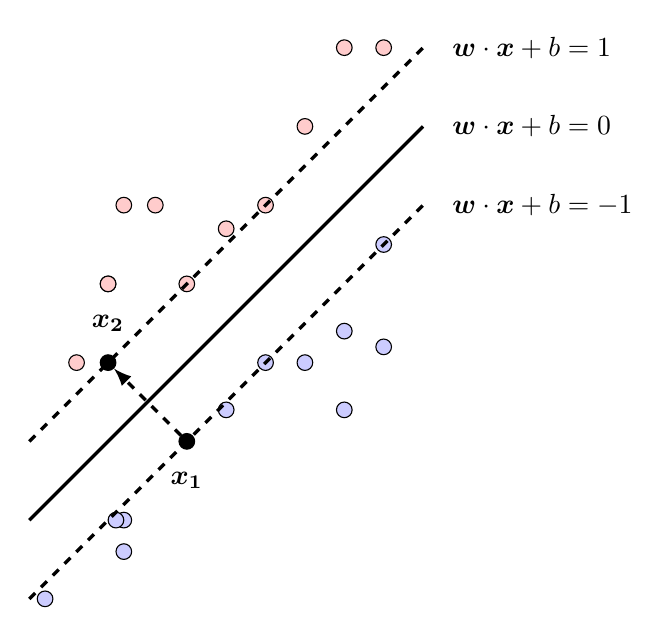
\begin{tikzpicture}
                        \node[sneg] at (2, 3) {};
                        \node[sneg] at (3, 4) {};
                        \node[sneg] at (1, 3) {};
                        \node[sneg] at (2.5, 3.7) {};
                        \node[sneg] at (1.2, 4) {};
                        \node[sneg] at (4.5, 6) {};
                        \node[sneg] at (3.5, 5) {};
                        \node[sneg] at (4, 6) {};
                        \node[sneg] at (1, 3) {};
                        \node[sneg] at (1.6, 4) {};
                        \node[sneg] at (0.6, 2) {};

                        \node[spos] at (4.5, 3.5) {};
                        \node[spos] at (3, 2) {};
                        \node[spos] at (4, 2.4) {};
                        \node[spos] at (2.5, 1.4) {};
                        \node[spos] at (1.2, 0) {};
                        \node[spos] at (4.5, 2.2) {};
                        \node[spos] at (3.5, 2) {};
                        \node[spos] at (4, 1.4) {};
                        \node[spos] at (1.2, -0.4) {};
                        \node[spos] at (1.1, 0) {};
                        \node[spos] at (0.2, -1) {};

                        \node[rbtb] (x1) at (2, 1) {};
                        \node[rbtb] (x2) at (1, 2) {};

                        \node at ($(x1) + (0, -0.5)$) {$\vec{x_1}$};
                        \node at ($(x2) + (0, 0.5)$) {$\vec{x_2}$};

                        \draw[very thick]
                        (0, 0) -- (5, 5)
                        (0, 1) edge[dashed] (5, 6)
                        (0, -1) edge[dashed] (5, 4)
                        (x1) edge[dashed, -latex] (x2);

                        \node[anchor=west] at (5.25, 6) {$\vec{w} \cdot \vec{x} + b = 1$};
                        \node[anchor=west] at (5.25, 5) {$\vec{w} \cdot \vec{x} + b = 0$};
                        \node[anchor=west] at (5.25, 4) {$\vec{w} \cdot \vec{x} + b = -1$};
                    \end{tikzpicture}
                \end{center}
                We want the margin between the two following lines to be as large as possible, and we can also derive the distance as follows;
                \begin{align*}
                    \vec{w} \cdot \vec{x} + b & = 1 \\
                    \vec{w} \cdot \vec{x} + b & = -1 \\
                    \vec{w} \cdot \vec{x_1} + b & = -1 & \text{let this be a point on the $-1$ plane} \\
                    \vec{w} \cdot (\vec{x_1} + m\vec{n}) + b & = 1 & \text{move the point along the normal by the size of the margin to $\vec{x_2}$} \\
                    m\vec{w} \cdot \vec{n} & = 2 & \text{from the previous two equations} \\
                    \vec{n} & = \frac{\vec{w}}{|| \vec{w} ||}
                \end{align*}
                SVM then aims to solve optimise the following;
                $$\max_{\vec{w}, b} \frac{2}{|| \vec{w} ||}$$
                This is subject to the following constraints, for all $i = 1, \dots, N$ (note that $y_i$ denotes the label of the point);
                \begin{align*}
                    \vec{w} \cdot \vec{x_i} + b & \geq 1 & \text{if } y_i = 1 \\
                    \vec{w} \cdot \vec{x_i} + b & \leq -1 & \text{if } y_i = -1
                \end{align*}

                However, we've assumed that all the points are linearly separable, which isn't always the case.
                In this case, we cannot solve the optimisation problem, since the constraints require the data to be linearly separable.
                This can be done with slack variables, $\xi_i \geq 0$ (for each data point).
                This formulates the optimisation problem as
                $$\min_{\vec{w}, b} || \vec{w} ||^2 + C\summation{i=1}{N} \xi_i$$
                Subject to the following, for all data points ($\forall i$);
                \begin{itemize}
                    \itemsep0em
                    \item $\xi_i \geq 0$
                    \item $y_i(\vec{w} \cdot \vec{x_i} + b) \geq 1 - \xi_i$
                \end{itemize}
                Note that $\xi_i$ will be 0 when the point is correctly classified or $0 < \xi_i \leq 1$ for points within the margin (but on the correct side of the hyperplane), otherwise it represents the distance from the margin.
                In the above, $C$ is a regularisation term (a small $C$ will allow constraints to easily be fulfilled, whereas a large $C$ would make constraints difficult to ignore - typically leading to a tighter margin).
            \subsubsection*{Optimisation}
                Note that we can formulate the slack variable as;
                $$\xi_i = \underbrace{\max(0, 1 - y_i(\vec{w} \cdot \vec{x_i} + b))}_\text{hinge loss}$$
                Therefore, we aim to optimise the following function;
                $$\min_{\vec{w}, b} || \vec{w} ||^2 + C\summation{i=1}{N} \max(0, 1 - y_i(\vec{w} \cdot \vec{x_i} + b))$$
                However, note that both of these functions (a quadratic term and a hinge loss function) are \textbf{convex} functions (hence we know there is a minimum, and that a local minimum is also a global minimum).
                Note that the non-negative weighted sum of two convex functions is also a convex function.
                A convex function $f : X \to R$ satisfies the following;
                $$\forall x_1, x_2 \in R,\ \forall t \in [0, 1]\ [f(tx_1 + (1 - t)x_2) \leq tf(x_1) + (1 - t)f(x_2)]$$
                A line joining $(x_1, f(x_1))$ and $(x_2, f(x_2))$ will lie \textbf{above} the function curve.
                There are two approaches to optimise this;
                \begin{itemize}
                    \itemsep0em
                    \item \textbf{gradient descent} \hfill used in large scale-optimisation
                        \smallskip

                        Note that the hinge loss function looks like the following;
                        \begin{center}
                            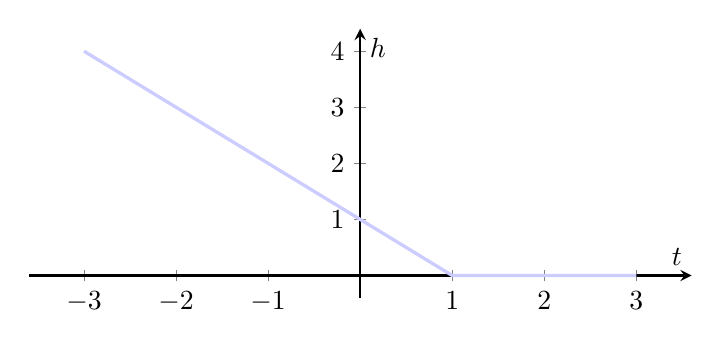
\begin{tikzpicture}
                                \begin{axis}[
                                    axis on top=false,
                                    axis line style=thick,
                                    domain=-3:3, samples=7,
                                    axis lines=middle, xlabel=$t$, ylabel=$h$,
                                    height=5cm, width=10cm,
                                    enlargelimits=true,
                                    xtick={-3,-2,...,3},
                                    ytick={0,...,4},
                                    xmin=-3, xmax=3,
                                    ymin=0, ymax=4
                                ]
                                    \addplot[very thick, blue!20] {max(0, 1 - \x)};
                                \end{axis}
                            \end{tikzpicture}
                        \end{center}
                        While it is not differentiable, we can use a more generalised concept for a gradient, the \textbf{subgradient};
                        $$\nabla_{\vec{w}}h = \begin{cases}
                            -y_i\vec{x_i} & \text{if } y_i(\vec{w} \cdot \vec{x_i} + b) < 1 \\
                            0 & \text{otherwise}
                        \end{cases}$$
                        This would be similar for $\nabla_bh$, however, we mainly focus on $\vec{w}$ for our derivation.
                        For each iteration, we move along the negative of the gradient by some step length $\eta$;
                        \begin{align*}
                            \vec{w}^{(k + 1)} & = \vec{w}^{(k)} - \eta\nabla_{\vec{w}}\left(|| \vec{w} ||^2 + C\summation{i=1}{N} \max(0, 1 - y_i(\vec{w} \cdot \vec{x_i} + b))\right) \\
                            & = \vec{w}^{(k)} - \eta\left(2\vec{w}^{(k)} + C \summation{i=1}{N} \nabla_{\vec{w}}h\right)
                        \end{align*}
                    \item \textbf{Lagrangian duality} (solves the dual problem) \hfill often used for SVM libraries
                        \smallskip

                        This is beyond the scope of the course, but works by solving the \textbf{dual} problem (given the \textbf{primal} problem).
                        See \textbf{CO343} for more details about duality.
                        \medskip

                        In the dual problem, the result of many of the $a_i$ are 0, except for the points located on the margin (the support vectors).
                        The solution of the primal problem is then given by;
                        $$\vec{w} = \summation{i = 1}{N} a_i y_i \vec{x_i}$$
                        $b$ can also be estimated with the support vectors by substituting back into the equation.
                \end{itemize}
            \subsubsection*{Classification}
                At test time, classification can be done according to;
                $$c = \begin{cases}
                    1 & \text{if } f(\vec{x}) = \vec{w} \cdot \vec{x} + b \geq 0 \\
                    -1 & \text{otherwise}
                \end{cases}$$
                This works quite well if the data can be linearly separable.
                However, if the points are not linearly separable in the \textbf{original} feature space, it may be easier to transform the features.
                Consider a dataset which has two classes, the first being a circle of points centred around some point $\vec{x_c}$, and another class being a ring of points around the first class.
                Using the transformation $\vec{Phi}(\vec{x}) = (\vec{x} - \vec{x_c})^2$, the first class would have a lower value (since it is closer to $\vec{x_c}$, which is then squared) after the transformation, whereas the second class would have a much higher value, thus separating the points.
                \medskip

                Therefore, if we transform the feature vector using a function $\vec{\Phi}$, the classifier also must change;
                $$f(\vec{x}) = \underbrace{\left(\summation{i}{} a_i y_i \vec{\Phi}(\vec{x_i})\right)}_\text{transformed $\vec{w}$} \cdot \vec{\Phi}\vec{x} + b$$
                We can also define the kernel (different from image filtering) as;
                $$\vec{k}(\vec{x_i}, \vec{x_j}) = \vec{\Phi}(\vec{x_i}) \cdot \vec{\Phi}(\vec{x_j})$$
                The classifier (which is now a non-linear function) only contains the kernel;
                $$f(\vec{x}) = \summation{i}{} a_i y_i \vec{k}(\vec{x_i}, \vec{x}) + b$$
                The common kernels used for SVM are;
                \begin{itemize}
                    \itemsep0em
                    \item \textbf{linear kernel}
                        $$\vec{k}(\vec{x_i}, \vec{x_j}) = \vec{x_i} \cdot \vec{x_j}$$
                    \item \textbf{polynomial kernel}
                        $$\vec{k}(\vec{x_i}, \vec{x_j}) = (\vec{x_i} \cdot \vec{x_j})^d \text{ or } (1 + \vec{x_i} \cdot \vec{x_j})^d$$
                    \item \textbf{Gaussian kernel / radial basis function (RBF) kernel}
                        $$\vec{k}(\vec{x_i}, \vec{x_j}) = e^{-\frac{|| \vec{x_i} - \vec{x_j} ||^2}{2 \sigma^2}}$$
                \end{itemize}
                Note that we only have binary classification at the moment.
                For multi-class classification, we can take several approaches (considering the MNIST digit recognition example);
                \begin{itemize}
                    \itemsep0em
                    \item \textbf{one versus rest}
                        \smallskip

                        In this, we train a classifier for each of the 10 digits, the first classifies between a digit that is 1 and not 1, the second being a classifier between 2 and not 2, and so on.
                        The classifier which produces the highest response at test time determines the result;
                        $$c = \argmax_{k = 1, \dots, K} f_k(\vec{x})$$
                    \item \textbf{one versus one}
                        \smallskip

                        In contrast to before, we have a classifier for each pairing of digits - for example, we'd have a classifier for 1 versus 2, 1 versus 3, 2 versus 3, and so on.
                        At test time, each classifier votes for the digit, and the majority vote wins.
                        The number of classifiers we need for $K$ classes is;
                        $$\frac{K(K - 1)}{2}$$
                \end{itemize}
        \subsection*{Lecture 14 - Image Classification III}
            Note that a lot of this is also covered in \textbf{CO395}.
            \subsubsection*{Neural Networks}
                Neural networks are an algorithm to learn a model from the data for classification / regression problems.
                Artificial neural networks are \textbf{inspired} by biology, but does not exactly model how a neuron works.
                In the past few decades, neural networks have improved with more layers of connections (deeper), as well has having better hardware for faster computation and larger datasets for training.
                \begin{center}
                    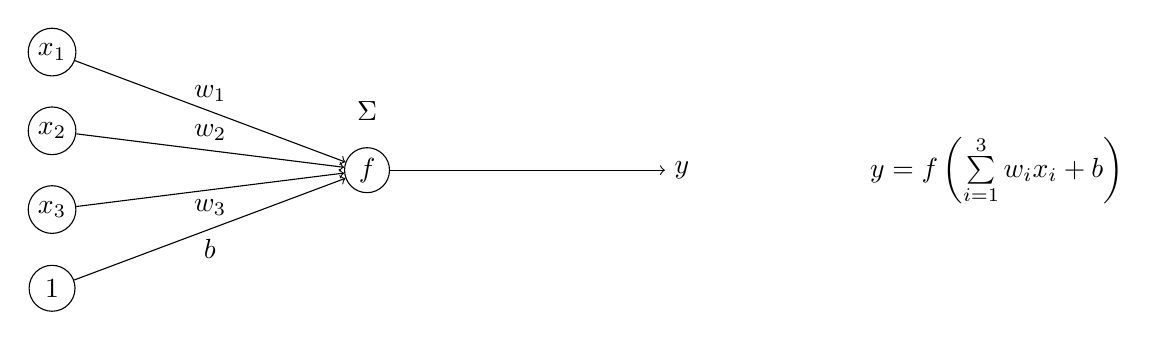
\begin{tikzpicture}
                        \node[circle, inner sep=2pt, draw] (x1) at (0, 0) {$x_1$};
                        \node[circle, inner sep=2pt, draw] (x2) at (0, -1) {$x_2$};
                        \node[circle, inner sep=2pt, draw] (x3) at (0, -2) {$x_3$};
                        \node[circle, inner sep=3pt, draw] (const) at (0, -3) {$1$};
                        \node[circle, inner sep=2pt, draw] (f) at (4, -1.5) {$f$};
                        \node (y) at (8, -1.5) {$y$};
                        \node at (4, -0.75) {$\Sigma$};
                        \node at (12, -1.5) {$y = f\left(\summation{i = 1}{3} w_i x_i + b\right)$};

                        \draw
                        (x1) edge[->, above] node{$w_1$} (f)
                        (x2) edge[->, above] node{$w_2$} (f)
                        (x3) edge[->, below] node{$w_3$} (f)
                        (const) edge[->, below] node{$b$} (f)
                        (f) edge[->] (y);
                    \end{tikzpicture}
                \end{center}
                The simplest form of a neural network is a perceptron, using which has a single layer and uses the \textbf{Heaviside} step function as an activation function (where $\vec{w}$ and $b$ are optimised to match the ground truth);
                $$y = \begin{cases}
                    1 & \text{if } \vec{w} \cdot \vec{x} + b > 0 \\
                    0 & \text{otherwise}
                \end{cases}$$
                Note that the difference (compared to SVMs) is that the non-linearity is added with an activation function $f(\vec{w} \cdot \vec{x} + b)$, whereas SVMs add non-linearity through feature transforms; $\vec{w} \cdot \vec{\Phi}(\vec{x}) + b$.
                A common activation function is the logistic function / sigmoid;
                $$f(z) = \frac{1}{1 + e^{-z}}$$
                A neural network is formed by connecting neurons, where the outputs of a neuron can be the inputs of another;
                \begin{center}
                    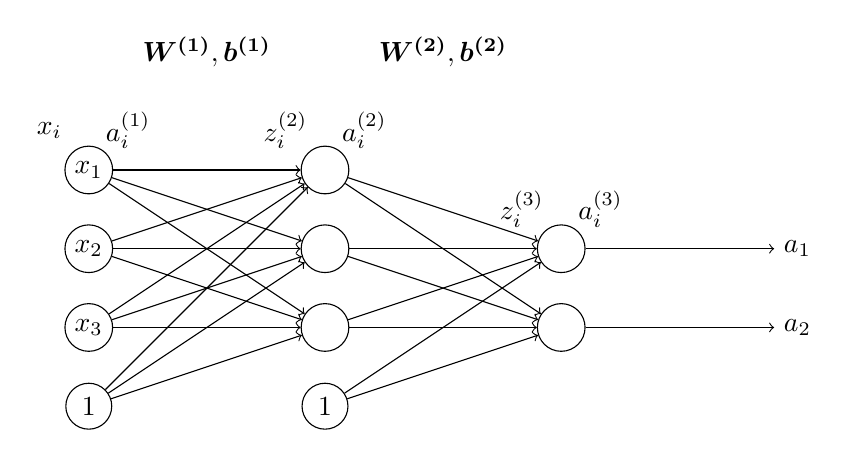
\begin{tikzpicture}
                        \node[circle, inner sep=2pt, draw] (x1) at (0, 0) {$x_1$};
                        \node[circle, inner sep=2pt, draw] (x2) at (0, -1) {$x_2$};
                        \node[circle, inner sep=2pt, draw] (x3) at (0, -2) {$x_3$};
                        \node[circle, inner sep=3pt, draw] (xc) at (0, -3) {$1$};
                        \node[circle, inner sep=2pt, draw] (h1) at (3, 0) {\phantom{$x_1$}};
                        \node[circle, inner sep=2pt, draw] (h2) at (3, -1) {\phantom{$x_2$}};
                        \node[circle, inner sep=2pt, draw] (h3) at (3, -2) {\phantom{$x_3$}};
                        \node[circle, inner sep=3pt, draw] (hc) at (3, -3) {$1$};
                        \node[circle, inner sep=2pt, draw] (o2) at (6, -1) {\phantom{$x_2$}};
                        \node[circle, inner sep=2pt, draw] (o3) at (6, -2) {\phantom{$x_3$}};
                        \node (a1) at (9, -1) {$a_1$};
                        \node (a2) at (9, -2) {$a_2$};

                        \draw
                        (x1) edge[->] (h1)
                        (x2) edge[->] (h1)
                        (x3) edge[->] (h1)
                        (xc) edge[->] (h1)
                        (x1) edge[->] (h2)
                        (x2) edge[->] (h2)
                        (x3) edge[->] (h2)
                        (xc) edge[->] (h2)
                        (x1) edge[->] (h3)
                        (x2) edge[->] (h3)
                        (x3) edge[->] (h3)
                        (xc) edge[->] (h3)
                        (h1) edge[->] (o2)
                        (h2) edge[->] (o2)
                        (h3) edge[->] (o2)
                        (hc) edge[->] (o2)
                        (h1) edge[->] (o3)
                        (h2) edge[->] (o3)
                        (h3) edge[->] (o3)
                        (hc) edge[->] (o3)
                        (o2) edge[->] (a1)
                        (o3) edge[->] (a2);

                        \node at (-0.5, 0.5) {$x_i$};
                        \node at (0.5, 0.5) {$a_i^{(1)}$};
                        \node at (2.5, 0.5) {$z_i^{(2)}$};
                        \node at (3.5, 0.5) {$a_i^{(2)}$};
                        \node at (5.5, -0.5) {$z_i^{(3)}$};
                        \node at (6.5, -0.5) {$a_i^{(3)}$};
                        \node at (1.5, 1.5) {$\mat{W^{(1)}}, \vec{b^{(1)}}$};
                        \node at (4.5, 1.5) {$\mat{W^{(2)}}, \vec{b^{(2)}}$};
                    \end{tikzpicture}
                \end{center}
                The output $a$ can be compared with the ground truth $y$ in a loss function $J$ (which we aim to minimise).
                A training set is denoted as pairs of data $\vec{x}$ and ground truth labels;
                $$\{(x_1, y_1), (x_2, y_2), \dots, (x_M, y_M)\}$$
                An example of a loss function is MSE;
                $$J(\vec{W}, \vec{b}) = \frac{1}{M} \summation{m = 1}{M} \frac{1}{2} ||a_m - y_m||^2$$
            \subsubsection*{Optimising}
                To calculate the output of a network $a$ given some input $x$, we use \textbf{forward propagation}.
                The parameters $\mat{W}$ and $\vec{b}$ can be found with gradient descent and \textbf{backpropagation} can be used to calculate the gradient.
                \medskip

                In the diagram above, we can perform a calculation as follows (applying the activation function to the input of each neuron) - this can also be more compactly written in matrix notation (where the activation function is generally applied element-wise);
                \begin{align*}
                    z_i^{(2)} & = W_{i, 1}^{(1)}a_1^{(1)} + W_{i, 2}^{(1)}a_2^{(1)} + W_{i, 3}^{(1)}a_3^{(1)} + b_i^{(1)} \\
                    a_i^{(2)} & = f\left(z_i^{(2)}\right) \\
                    \vec{z^{(2)}} & = \mat{W^{(1)}}\vec{a^{(1)}} + \vec{b^{(1)}} \\
                    \vec{a^{(2)}} & = f\left(\vec{z^{(2)}}\right)
                    \intertext{More generally, for layer $l + 1$, we do the following;}
                    \vec{z^{(l + 1)}} & = \mat{W^{(l)}}\vec{a^{(l)}} + \vec{b^{(l)}} \\
                    \vec{a^{(l + 1)}} & = f\left(\vec{z^{(l + 1)}}\right)
                \end{align*}
                Gradient descent can be done as follows, given a learning rate $\alpha$ (note the equals here denotes reassignment, rather than equality);
                \begin{align*}
                    \mat{W} & = \mat{W} - \alpha \pdif{J}{\mat{W}} \\
                    \vec{b} & = \vec{b} - \alpha \pdif{J}{\vec{b}}
                \end{align*}
                The backpropagation algorithm is based on the chain rule.
                We can work out the derivative of a composition as follows;
                \begin{align*}
                    z & = g(f(x)) \\
                    y & = f(x) \\
                    z & = g(y) \\
                    \dif{z}{x} & = \dif{z}{y} \dif{y}{x}
                \end{align*}
                Using the running example, we can quite easily derive $\pdif{J}{a}$, as well as $\pdif{a}{\mat{W^{(2)}}}$.
                Therefore, we can use the chain rule;
                $$\pdif{J}{\mat{W^{(2)}}} = \pdif{J}{a} \pdif{a}{\mat{W^{(2)}}}$$
            \subsubsection*{Stochastic Gradient Descent}
                SGD addresses the computational expense of performing forward and backward propagation for all samples in one go.
                In SGD, a batch of $B$ samples are selected for performing the propagation.
                For each iteration in the optimisation, we do the following;
                \begin{enumerate}[1.]
                    \itemsep0em
                    \item randomly select a batch of $B$ samples
                    \item calculate the gradients $\pdif{J_B}{\mat{W}}$ and $\pdif{J_B}{\vec{b}}$ for \textbf{only} this batch
                    \item update the parameters (note that $J_B$ denotes the loss for the $B$ samples)
                        \begin{align*}
                            \mat{W} & = \mat{W} - \alpha \pdif{J_B}{\mat{W}} \\
                            \vec{b} & = \vec{b} - \alpha \pdif{J_B}{\vec{b}}
                        \end{align*}
                \end{enumerate}
            \subsubsection*{Classification}
                Note that MSE works for regression problems, where $y$ is a continuous variable.
                However, this isn't optimal for classification problems, which can be binary ($y$ is 1 or 0) or multi-class (where $y$ is one of a number of classes).
                \medskip

                In binary classification, we only need a single neuron in the output layer.
                The activation function could be the sigmoid function, which gives an output $\in (0, 1)$, which is in the range of probability.
                Consider the case where we predict a probability of $0.9$ for class 1 (hence $0.1$ for class 0).
                The ground truth has $y = 1$ (therefore the probability of class 1 is 1, and class 0 is 0).
                A distance metric between the predicted probability and true probability can be used, namely cross entropy.
                \medskip

                The cross entropy between a true probability distribution $p$ and an estimated probability distribution $q$ is;
                $$H(p, q) = -\summation{i}{} p_i\log(q_i)$$
                In the general case (for two classes), we have $p = [y, 1 - y]$ and $q = [f(z), 1 - f(z)]$, hence;
                $$H(p, q) = -[y\log(f(z)) + (1 - y)\log(1 - f(z))]$$
                For $K$ classes, there are $K$ neurons in the output layer.
                The activation function used would be softmax, to create a probability distribution;
                $$f(z_i) = \frac{e^{z_i}}{\summation{k = 1}{K} e^{z_k}}$$
                The true probability is represented with one-hot (only one element is 1) encoding;
                $$p = [y_1, \dots, y_i, \dots, y_K] = [0, \dots, 1, \dots, 0]$$
            \subsubsection*{Performance}
                To create more training samples, data augmentation can be performed.
                This applies affine transformations to the original samples, by performing translation, scaling, squeezing, and shearing.
                \medskip

                Note that a key limitation of MLP is the high number of parameters required.
                As such, it's likely to scale poorly for larger images (and even more so if more channels are considered).
                This is caused by the flattening of a 2D image into a single vector, rather than performing operators on 2D images.
        \subsection*{Lecture 15 - Image Classification IV}
            \subsubsection*{Convolutional Neural Networks}
                In contrast to MLPs, CNNs assume inputs of 2D images and encode properties such as local connectivity and weight sharing into the architecture, reducing the number of parameters and making the computation more efficient.
                \medskip

                When we look at an image, we first look at local regions, process this information, and then combine information from different regions to form a global understanding.
                In CNNs, each neuron will only see a \textbf{receptive field} (small local region) in the layer before it - this is also called local connectivity (reducing the number of parameters).
                \begin{center}
                    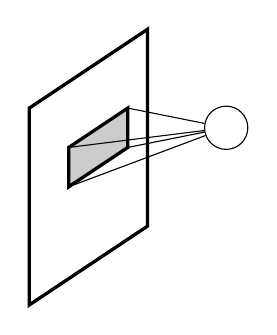
\begin{tikzpicture}[x=0.5cm, y=0.5cm]
                        \draw[very thick] (0, 0) -- (3, 2) -- (3, -3) -- (0, -5) -- cycle;
                        \draw[very thick, fill=black!20] (1, -1) -- (2.5, 0) -- (2.5, -1) -- (1, -2) -- cycle;
                        \node[draw, circle, inner sep=3pt] (n) at (5, -0.5) {\phantom{$x$}};

                        \draw
                        (1, -1) -- (n)
                        (2.5, 0) -- (n)
                        (2.5, -1) -- (n)
                        (1, -2) -- (n);
                    \end{tikzpicture}
                \end{center}
                Note in the example above, a neuron only depends on a small region in the previous layer, whereas a fully connect layer in an MLP depends on \textbf{all} the neurons in the previous layer.
            \subsubsection*{Convolutional Layer}
                In a CNN, convolutional layers are the basic building blocks.
                Consider an input image of size $X \times Y \times C$ (note that $C$ denotes the number of channels, 3 for RGB, and 1 for greyscale).
                If a neuron required a $5 \times 5 \times C$ cuboid of the input, it would have $5 \times 5 \times C + 1$ parameters (including one for bias).
                \medskip

                The input and output of the neuron are defined as follows (note that here we sum over 3 axes);
                \begin{align*}
                    z & = \summation{i, j, k}{} \mat{W}_{i, j, k} \vec{x}_{i, j, k} + b \\
                    a & = f(z)
                \end{align*}
                However, we can add more neurons to form a $D \times 1 \times 1$ cuboid of output (where $D$ represents the depth).
                Each of these neurons has its own set of weights and biases;
                $$a_n = f\left(\summation{i, j, k}{} \mat{W_n}_{i, j, k} \vec{x}_{i, j, k} + b_n\right)$$
                This window can be moved across the input image, which gives an output cuboid of size $X \times Y \times D$ - note that all of the windows use the same weights, allowing us to have a total of $5 \times 5 \times C \times D$ parameters for connection weights, and another $D$ for bias.
                The convolutional kernel $\mat{W}$ has four dimensions - \blue{output depth}, \violet{kernel width}, \teal{kernel height}, \red{input depth};
                $$a_d = f\left(\summation{i, j, k}{} \mat{W}_{\blue{d}, \violet{i}, \teal{j}, \red{k}}\vec{x}_{\violet{i}, \teal{j}, \red{k}} + b_{\blue{d}}\right)$$
                The output feature map has three dimensions, the output depth, as well as the width and height.
                \medskip

                We can set a number of parameters for the layer;
                \begin{itemize}
                    \itemsep0em
                    \item \textbf{padding}
                        \smallskip

                        Recall that applying a $3 \times 3$ kernel on an image of shape $X \times Y$ will result in an output of $(X - 2) \times (Y - 2)$.
                        Adding a padding of $p = 1$ gives a border of zeroes around the image.
                        Given an input shape of $X_\text{in} \times Y_\text{in}$, a $k \times k$ kernel, $p \times p$ padding, we obtain the following output shape;
                        $$X_\text{out} = X_\text{in} + 2p - k + 1$$
                    \item \textbf{stride}
                        \smallskip

                        In order to move the window faster and obtain a downsampled grid, we can use a stride.
                        For example, with $s = 2$, it the window to every other pixel.
                        Consider the following; note that we have a padding $p = 1$ and stride $s = 2$ (crosses denote the centre of the kernel);
                        \begin{center}
                            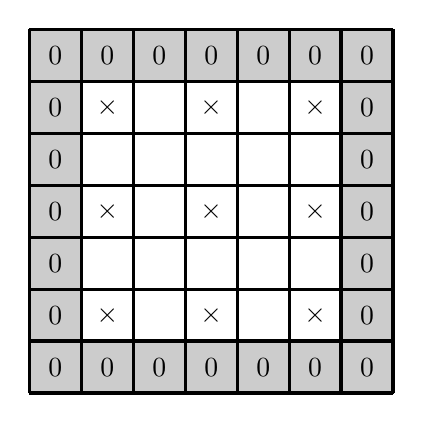
\begin{tikzpicture}[x=0.66cm, y=0.66cm]
                                \foreach \x in {0,...,6} {
                                    \draw[fill=black!20] (\x, 0) -- (\x, 1) -- (\x + 1, 1) -- (\x + 1, 0) -- cycle;
                                    \node at (\x + 0.5, 0.5) {$0$};
                                    \draw[fill=black!20] (\x, 6) -- (\x, 7) -- (\x + 1, 7) -- (\x + 1, 6) -- cycle;
                                    \node at (\x + 0.5, 6.5) {$0$};
                                }
                                \foreach \y in {1,...,5} {
                                    \draw[fill=black!20] (0, \y) -- (0, \y + 1) -- (1, \y + 1) -- (1, \y) -- cycle;
                                    \node at (0.5, \y + 0.5) {$0$};
                                    \draw[fill=black!20] (6, \y) -- (6, \y + 1) -- (7, \y + 1) -- (7, \y) -- cycle;
                                    \node at (6.5, \y + 0.5) {$0$};
                                }
                                \foreach \x in {0,...,7} {
                                    \draw[very thick] (\x, 0) -- (\x, 7);
                                }
                                \foreach \y in {0,...,7} {
                                    \draw[very thick] (0, \y) -- (7, \y);
                                }
                                \node at (1.5, 1.5) {$\times$};
                                \node at (3.5, 1.5) {$\times$};
                                \node at (5.5, 1.5) {$\times$};
                                \node at (1.5, 3.5) {$\times$};
                                \node at (3.5, 3.5) {$\times$};
                                \node at (5.5, 3.5) {$\times$};
                                \node at (1.5, 5.5) {$\times$};
                                \node at (3.5, 5.5) {$\times$};
                                \node at (5.5, 5.5) {$\times$};
                            \end{tikzpicture}
                        \end{center}
                        This can be combined with the padding shape to obtain the following (given a stride of $s \times s$);
                        $$X_\text{out} = \left\lfloor\frac{X_\text{in} + 2p - k}{s}\right\rfloor + 1$$
                    \item \textbf{dilation}
                        \smallskip

                        For a neuron to have a larger receptive field, we can either keep the kernel size the same (but downsample the input image), or increase the kernel size (thus also increasing the number of parameters).
                        Dilation aims to increase the region size without downsampling or adding more parameters.
                        Consider the following - note that a \violet{violet} cross denotes the centre of the kernel, and regular crosses denote points which are taken into account (this is a $3 \times 3$ kernel, with dilation $d = 2$, hence we look at every other pixel);
                        \begin{center}
                            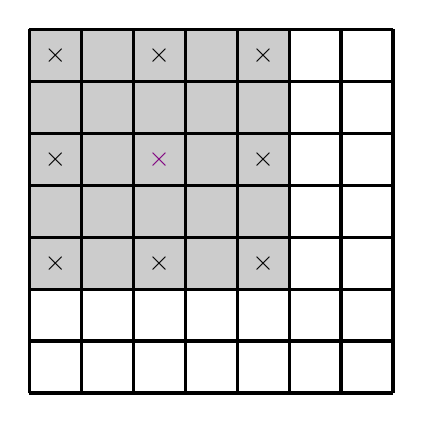
\begin{tikzpicture}[x=0.66cm, y=0.66cm]
                                \draw[fill=black!20] (0, 7) -- (5, 7) -- (5, 2) -- (0, 2) -- cycle;
                                \foreach \x in {0,...,7} {
                                    \draw[very thick] (\x, 0) -- (\x, 7);
                                }
                                \foreach \y in {0,...,7} {
                                    \draw[very thick] (0, \y) -- (7, \y);
                                }
                                \node at (2.5, 4.5) {\violet{$\times$}};
                                \node at (0.5, 6.5) {$\times$};
                                \node at (2.5, 6.5) {$\times$};
                                \node at (4.5, 6.5) {$\times$};
                                \node at (0.5, 4.5) {$\times$};
                                \node at (4.5, 4.5) {$\times$};
                                \node at (0.5, 2.5) {$\times$};
                                \node at (2.5, 2.5) {$\times$};
                                \node at (4.5, 2.5) {$\times$};
                            \end{tikzpicture}
                        \end{center}
                \end{itemize}
            \subsubsection*{Pooling Layer}
                A pooling layer is another building block of CNNs, which make feature maps / representations smaller (similar to image downsampling).
                Consider the following example, which performs max pooling with a $2 \times 2$ window and stride of 2;
                \begin{center}
                    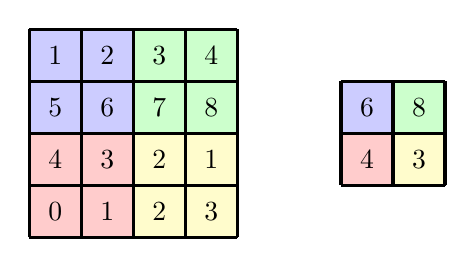
\begin{tikzpicture}[x=0.66cm, y=0.66cm]
                        \draw[fill=blue!20] (0, 2) -- (0, 4) -- (2, 4) -- (2, 2) -- cycle;
                        \draw[fill=green!20] (2, 2) -- (2, 4) -- (4, 4) -- (4, 2) -- cycle;
                        \draw[fill=red!20] (0, 0) -- (0, 2) -- (2, 2) -- (2, 0) -- cycle;
                        \draw[fill=yellow!20] (2, 0) -- (2, 2) -- (4, 2) -- (4, 0) -- cycle;
                        \foreach \x in {0,...,4} {
                            \draw[very thick] (\x, 0) -- (\x, 4);
                        }
                        \foreach \y in {0,...,4} {
                            \draw[very thick] (0, \y) -- (4, \y);
                        }
                        \begin{scope}[shift={(0.5, 0.5)}]
                            \node at (0, 0) {$0$};
                            \node at (1, 0) {$1$};
                            \node at (2, 0) {$2$};
                            \node at (3, 0) {$3$};
                            \node at (0, 1) {$4$};
                            \node at (1, 1) {$3$};
                            \node at (2, 1) {$2$};
                            \node at (3, 1) {$1$};
                            \node at (0, 2) {$5$};
                            \node at (1, 2) {$6$};
                            \node at (2, 2) {$7$};
                            \node at (3, 2) {$8$};
                            \node at (0, 3) {$1$};
                            \node at (1, 3) {$2$};
                            \node at (2, 3) {$3$};
                            \node at (3, 3) {$4$};
                        \end{scope}
                        \begin{scope}[shift={(6, 1)}]
                            \draw[fill=blue!20] (0, 1) -- (0, 2) -- (1, 2) -- (1, 1) -- cycle;
                            \draw[fill=green!20] (1, 1) -- (1, 2) -- (2, 2) -- (2, 1) -- cycle;
                            \draw[fill=red!20] (0, 0) -- (0, 1) -- (1, 1) -- (1, 0) -- cycle;
                            \draw[fill=yellow!20] (1, 0) -- (1, 1) -- (2, 1) -- (2, 0) -- cycle;
                            \draw[very thick]
                            (0, 0) -- (2, 0)
                            (0, 1) -- (2, 1)
                            (0, 2) -- (2, 2)
                            (0, 0) -- (0, 2)
                            (1, 0) -- (1, 2)
                            (2, 0) -- (2, 2);
                            \begin{scope}[shift={(0.5, 0.5)}]
                                \node at (0, 0) {$4$};
                                \node at (1, 0) {$3$};
                                \node at (0, 1) {$6$};
                                \node at (1, 1) {$8$};
                            \end{scope}
                        \end{scope}
                    \end{tikzpicture}
                \end{center}
                Another form of pooling is average pooling.
            \subsubsection*{LeNet-5}
                This uses 7 layers in total (including the output layer but excluding the input layer).
                A layer beginning with C denotes a convolutional layer, S denotes a pooling (subsampling) layer, and F denotes a fully connected layer.
                The input image is of size $32 \times 32$.
                \begin{itemize}
                    \itemsep0em
                    \item C1 \hfill $28 \times 28$ with depth of 6, using $5 \times 5$ convolutions
                    \item S2 \hfill $14 \times 14$ with depth of 6, max pooling
                    \item C3 \hfill $10 \times 10$ with depth of 16, using $5 \times 5$ convolutions
                    \item S4 \hfill $5 \times 5$ with depth of 16
                    \item C5 \hfill 120 neurons
                    \item F6 \hfill 84 neurons
                    \item output \hfill 10 classes
                \end{itemize}
                The same techniques can be used to optimise a loss function, as convolutional layers are mathematically similar to layers in MLP (just with more dimensions).
            \subsubsection*{Deep Neural Networks}
                A factor in the improvement of deep neural networks is hardware; namely GPUs.
                They are ideal for training neural networks as convolutional operations can be performed in parallel using thousands of simpler (relative to CPU) cores on a GPU.
                \medskip

                Another factor is improvements in optimisation.
                There are two main problems with previously mentioned approach; exploding gradient (where the gradient becomes too large for the algorithm to converge) and vanishing gradient (where the gradient becomes too small for the weights to change values).
                An example of exploding gradient is when the current point is very close to a `cliff' - the gradient descent may overshoot up the cliff, causing it to not converge.
                One solution is to perform gradient clipping (by value), which does the following for each element of the gradient $\vec{g}$;
                $$g_i = \begin{cases}
                    v_\text{min} & \text{if } g_i < v_\text{min} \\
                    v_\text{max} & \text{if } g_i > v_\text{max} \\
                    g_i & \text{otherwise}
                \end{cases}$$
                Another approach is to clip by the $\ell_2$-norm;
                $$\vec{g} = \begin{cases}
                    \frac{\vec{g}}{|| \vec{g} ||}v & \text{if } || \vec{g} || > v \\
                    \vec{g} & \text{otherwise}
                \end{cases}$$
                On the other hand, the vanishing gradient problem can be caused on either extremes of the sigmoid function.
                Recall that gradients are multiplied, therefore if any are zero (or close to zero), the propagated derivative will also be small;
                \begin{align*}
                    f(z) & = \frac{1}{1 + e^{-z}} & \text{sigmoid function} \\
                    f^\prime(z) & = \frac{e^{-z}}{(1 + e^{-z})^2} \\
                    & = f(z) (1 - f(z)) & \text{small if either are close to 0 or 1} \\
                    \pdif{J}{\vec{z^{(l)}}} & = \left(\left(\mat{W^{(l)}}\right)^\top \pdif{J}{\vec{z^{(l + 1)}}}\right) \circ f^\prime\left(\vec{z^{(l)}}\right) & \text{propagated derivative}
                \end{align*}
                This can be addressed with different activation functions, for example;
                \begin{itemize}
                    \itemsep0em
                    \item \textbf{rectified linear unit (ReLU)}
                        $$f(z) = \begin{cases}
                            0 & z < 0 \\
                            z & z \geq 0
                        \end{cases}$$
                        This gives the following subgradient;
                        $$f^\prime(z) = \begin{cases}
                            0 & z < 0 \\
                            1 & z \geq 0
                        \end{cases}$$
                        This prevents gradients from vanishing when $z$ is large, however it becomes 0 with a negative $z$.
                        This outperforms sigmoid as an activation function for deep neural networks.
                    \item \textbf{leaky ReLU}
                        $$f(z) = \begin{cases}
                            0.01z & z < 0 \\
                            z & z \geq 0
                        \end{cases}$$
                        Similar to ReLU, but gives some gradient for negative values,
                    \item \textbf{parametric ReLU (PReLU)}
                        $$f(z) = \begin{cases}
                            az & z < 0 \\
                            z & z \geq 0
                        \end{cases}$$
                        This is similar to leaky ReLU, however the parameter $a$ is learnt in training.
                    \item \textbf{exponential linear unit (ELU)}
                        $$f(z) = \begin{cases}
                            a(e^z - 1) & z < 0 \\
                            z & z \geq 0
                        \end{cases}$$
                \end{itemize}
            \subsubsection*{AlexNet and VGG}
                AlexNet is generally quite similar to LeNet, but is deeper.
                It also uses ReLU for activation, and performs data augmentation by cropping random $224 \times 224$ regions from the original $256 \times 256$ images, as well as performing horizontal reflection and perturbing RGB values.
                \medskip

                VGG only uses $3 \times 3$ convolutional kernels, rather than larger kernels.
                The convolution of two $3 \times 3$ kernels is equivalent to a $5 \times 5$, three kernels is equivalent to $7 \times 7$, and so on - this is deeper and reduces the number of parameters.
                In addition, more non-linearity can be added as activation functions can be used after every small kernel.
        \subsection*{Lecture 16 - Object Detection}
            When we formulate the problem for image classification, we develop a classifier which analyses the input image and gives a class label as an output (which may give some probability of it being a certain class).
            However, with object detection, we want to develop a detector which tells us the label, but also a bounding box $(x, y, w, h)$, which specifies the top left (or centre) and the size of the box.
            \medskip

            We've built a neural network that can perform classification.
            If we move a sliding window across a large image, and move a sliding window across the image (treating the windows as smaller images), we can find regions.
            At each window, we perform two tasks;
            \begin{itemize}
                \itemsep0em
                \item classification (e.g. whether this is an animal or not)
                \item localisation (bounding box coordinates) - the sliding window already gives some localisation, however we want to refine this with CNN features
            \end{itemize}
            The CNN gives an output with two branches; the first is fully connected to $K$ classes (which provides a class score) compared against the ground truth class label (with cross entropy), and another fully connected to the four variables of the bounding box, which is compared against the ground truth bounding box.
            These are then added together to be optimised.
            \medskip

            However, it may be expensive to apply a CNN to each pixel location on the image.
            Object detection is split into two-stage detection;
            \begin{itemize}
                \itemsep0em
                \item \textbf{region proposal} \hfill initial guesses to propose some possible interesting regions
                \item \textbf{detector} \hfill apply network to classify and predict bounding boxes of these regions
            \end{itemize}
            One-stage detection skips guessing, but rather divides the image into grid cells, and then performs classification and bounding on these cells.
            \subsubsection*{Selective Search}
                This is rarely used nowadays and is a traditional approach before the development of CNNs.
                We can look at image features such as greyscale intensities or gradients to separate the image into regions with similar features.
            \subsubsection*{Faster R-CNN}
                A region proposal network (RPN) is used instead (which is much faster compared to selective search).
                The input image is fed into a convolutional network, which gives a feature map describing the image.
                This then goes into a region proposal network which gives interesting regions to be looked at.
                In stage 2, there is a classifier / detector which looks closely at the proposed regions, and can also refine the shape of the bounding box.
                \medskip

                AlexNet / VGG-16 are known as backbone networks (and are often pretrained), with the last convolutional layer being used as a convolutional feature map.
                Both stages rely on this feature map.
                Each pixel of the feature map is a high-dimensional feature vector, describing the content of a small region in the input image (which may tell us whether a region is interesting).
                \medskip

                Using this feature map (such as ~conv5~ in VGG), we can use a $3 \times 3$ sliding window to perform binary classification at each location, giving it 0 if it isn't interesting, and 1 if it is.
                It handles objects of different sizes / aspect ratio by making $k$ predictions (bounding boxes).
                For example, this is done in 3 scales $128^2, 256^2, 512^2$, and 3 aspect ratios $1:1, 1:2, 2:1$ - these bounding boxes are called anchors.
                For a convolutional feature map of $W \times H$, $W \times H \times k$ anchors are predicted (in our case $k = 9 = 3 \times 3$) - only the highest scoring boxes are kept (based on objectness score, generated by the network).
                \medskip

                The loss is defined as;
                $$L(p, t) = \underbrace{\summation{i = 1}{n_\text{anchor}} L_\text{cls}(p_i, p_i^*)}_\text{classification loss} + \lambda \underbrace{\summation{i = 1}{n_\text{anchor}} 1_{y = 1}L_\text{loc}(t_i, t_i^*)}_\text{localisation loss}$$
                The classification loss function $L_\text{cls}$ is can be calculated with cross entropy, by comparing the predicted objectness score $p_i$ with the ground truth $p_i^*$ (a binary value, 1 for a interesting location and 0 otherwise).
                The localisation loss attempts to refine the bounding box.
                We can either directly predict the values for a bounding box (the centre coordinates $x, y$ and size $w, h$), or the transformation parameters $\vec{t}$ from the anchor into the ground truth bounding box (note that if $\vec{t} = \vec{0}$, then the predicted bounding box is equivalent to the anchor);
                \begin{align*}
                    \text{anchor} & = (x_a, y_a, w_a, h_a) \\
                    \text{predicted bounding box} & = (x, y, w, h) \\
                    \text{predicted transformation} & = (t_x, t_y, t_w, t_h) \\
                    t_x & = \frac{x - x_a}{w_a} \\
                    t_y & = \frac{y - y_a}{h_a} \\
                    t_w & = \log\left(\frac{w}{w_a}\right) \\
                    t_g & = \log\left(\frac{h}{h_a}\right)
                \end{align*}
                It may be easier to predict the transformation than the bounding box directly, since the predicted bounding box components may be arbitrary.
                Note that the localisation loss compares vectors of continuous numbers, therefore MSE can be used as the loss function.
                \medskip

                Now that we have the locations and sizes of the objects, we can look closely at them in the feature map.
                The features from the region (which is no longer just a $3 \times 3$ window) can be used in a classifier (RoI pooling).
                In the RoI (region of interest) pooling layer, the location and size is calculated on the feature map - the features in this region are then converted into a fixed size to be provided into the classifier.
                \medskip

                For each RoI, the classifier predicts the label class and refines the bounding box estimate;
                $$L(p, t) = L_\text{cls}(p, y) + \lambda \cdot 1_{y \geq 0} L_\text{loc}(t, t^*)$$
                Note that the classification loss is now a multi-class classification problem.
                \medskip

                RPN and detection network are fairly similar.
                However, the input to a RP is a $3 \times 3$ window, whereas the input to a detection network is a proposed region (leading to more accurate features).
                RPN is also class-agnostic (a binary value for whether the region is interesting or not) whereas the detection network classifies the region into a number of classes.
                The detection network doesn't need anchors (since we have a rough size from the proposal), whereas RPN does since we do not know the shape of the object.
            \subsubsection*{One-Stage Object Detection}
                Region proposal and classification can be done in a single go with one-stage object detection methods, such as YOLO and SSD.
                The region proposal network, in two-stage, uses a binary value for the classification loss.
                This is changed into a multi-class classifier, which predicts the object for each anchor.
                \medskip

                Note that Faster R-CNN is more accurate but slower, and vice versa for SSD.
                Faster R-CNN is more accurate as it first roughly estimates the region size, before looking closely at features and then refining it.
            \subsubsection*{Performance}
                Note that backbone networks can be changed out to improve performance.
                The meta architecture (Faster RCNN, R-FCN, SSD, etc.) combined with the backbone network can be used to observe trade-offs between speed and accuracy.
        \subsection*{Lecture 17 - Image Segmentation}
            This is an even more detailed understanding than a bounding box; where there is a label class for each pixel (0 for background, etc.) - this can generate a segmentation mask.
            Instance segmentation gives each instance (such as each person) a unique label.
            \subsubsection*{Thresholding}
                This is one of the simplest methods for segmentation, and converts a greyscale image into a binary label map.
                At each pixel, the label is defined as follows;
                $$f(x) = \begin{cases}
                    1 & \text{if } I(x) \geq \text{threshold} \\
                    0 & \text{otherwise}
                \end{cases}$$
                This requires no training data, and the only parameter we require is the threshold.
                This relies on the intensity histogram being split into two classes, which can easily be split with a threshold.
            \subsubsection*{K-means}
                Generally, there can be more than two classes.
                K-means can provide a simple method for clustering by estimating cluster parameters.
                Each cluster can be represented by its centre, with each data point (pixel intensity) being associated to the nearest centre.
                The optimal centres minimise the intra-class variance (note $C_k$ denotes data points which are associated with cluster $k$);
                $$\min \summation{k = 1}{K} \summation{x \in C_k}{} (x - \mu_k)^2$$
                This can be reformulated with $\delta_{x, k}$, which denotes membership (whether $x$ is assigned to cluster $k$ or not) - the two unknowns are the membership and the cluster centre.
                $$\min \summation{k = 1}{K} \summation{x}{} \delta_{x, k}(x - \mu_k)^2$$
                If we know $\delta_{x, k}$ (the association between data and clusters), we can work out $\mu_k$, and vice versa.
                However, we don't know either of these initially.
                \medskip

                This can be done iteratively, by taking some initial guess for \textbf{either} of these parameters.
                The algorithm is already covered in \textbf{CO395} (take initial guess for cluster centres, compute $\delta_{x, k}$, update $\mu_k$, and so on).
                \medskip

                In order to determine the number of clusters ($K$), we can calculate the intra-class variance for each value of $K$.
                The clustering can also be performed on other features, such as colour similarity (possibly combined with position).
                $x$ becomes a feature vector, rather than a scalar.
            \subsubsection*{Gaussian Mixture Model (GMM)}
                K-means performs a hard assignment of a data point $x$ to a cluster $k$.
                GMMs allow for soft assignment by assuming each cluster is a Gaussian distribution.
                The probability that $x_j$ is in cluster $k$ is;
                $$P(y_j = k\ |\ x_i, \pi_k, \mu_k, \sigma_k) = \pi_k \cdot \frac{1}{\sqrt{2 \pi}\sigma_k} e^{-\frac{(x - \mu_k)^2}{2\sigma_k^2}}$$
                The process for updating this is very similar to K-means (algorithm is detailed in \textbf{CO395} again).
                The parameters are updated as follows ($j \in [1, N]$);
                \begin{align*}
                    \pi_k & = \frac{\summation{j}{} P(y_j = k)}{N} \\
                    \mu_k & = \frac{\summation{j}{} P(y_j = k) \cdot x_j}{\summation{j}{} P(y_j = k)} \\
                    \sigma^2_k & = \frac{\summation{j}{} P(y_j = k) \cdot (x_j - \mu_k)^2}{\summation{j}{} P(y_j = k)} \\
                \end{align*}
                The class is then assigned by maximum probability;
                $$c = \argmax_c P(y_j = c\ |\ x_j, \pi_c, \mu_c, \sigma_c)$$
                This method is used in \textit{Microsoft PowerPoint}, which as two clusters ($K = 2$).
                Segmentation is then performed with constraints (such as smoothness, or user editing using GrabCut).
            \subsubsection*{CNNs}
                The pixel-wise segmentation map will have to manually be annotated by humans (which can be used as ground truth).
                For simplicity, we assume we have this data (pairs of images with their respective segmentation maps).
                The ideas are the same as before; moving a window across an image and applying the classification network to each pixel.
                However, applying the network to many windows is expensive - we would rather develop a network which provides a pixel-wise probability map (rather than single probability vectors).
                \medskip

                The last feature map (before the fully connected layers) of AlexNet is of size $13 \times 13$, downsampled by a factor of $16$ from $224 \times 224$.
                Each pixel in this feature map encodes information regarding a $16 \times 16$ region in the input image.
                Instead of using fully connected layers to obtain probability vectors, we can obtain pixel-wise classification results from the feature map.
                A process called \textbf{convolutionalization} replaces the fully connected layers with convolutional layers (hence creating a fully convolutional network) to enable the network to produce a pixel-wise probability map (each class will have a heat map, whereas before a class would be a single value in the probability vector).
                Note that the depth of the final convolutional network represents the number of classes (the ground truth would be one-hot encoded heat maps).
                \medskip

                Note that we will need to apply an upsampling operation to obtain a pixel-wise prediction (since the feature map is downsampled).
                A transposed convolution can be used to achieve this.
                Consider the following, which has a stride of 2 (the windows jump by 2) - each pixel in the input contributes to a $3 \times 3$ window in the output, with some weights;
                \begin{center}
                    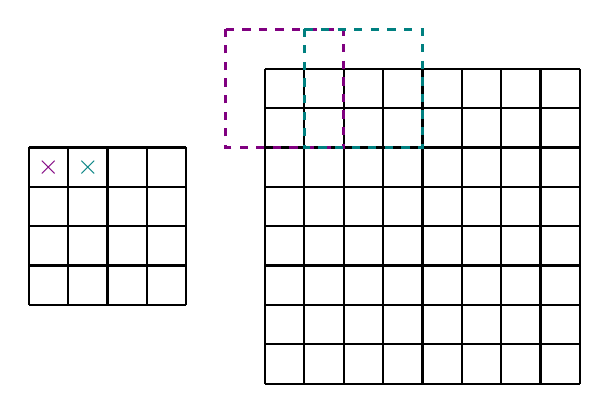
\begin{tikzpicture}[x=0.5cm, y=0.5cm]
                        \foreach \x in {0,...,4} {
                            \draw[thick] (\x, 0) -- (\x, 4);
                        }
                        \foreach \y in {0,...,4} {
                            \draw[thick] (0, \y) -- (4, \y);
                        }

                        \begin{scope}[shift={(6, -2)}]
                            \foreach \x in {0,...,8} {
                                \draw[thick] (\x, 0) -- (\x, 8);
                            }
                            \foreach \y in {0,...,8} {
                                \draw[thick] (0, \y) -- (8, \y);
                            }
                        \end{scope}

                        \node[violet] at (0.5, 3.5) {$\times$};
                        \node[teal] at (1.5, 3.5) {$\times$};

                        \draw[very thick, violet, dashed] (5, 7) -- (8, 7) -- (8, 4) -- (5, 4) -- cycle;
                        \draw[very thick, teal, dashed] (7, 7) -- (10, 7) -- (10, 4) -- (7, 4) -- cycle;
                    \end{tikzpicture}
                \end{center}
                A convolution in 1D can be represented as follows (note that the input is $\vec{x}$, which denotes a vertical region, and the kernel is a $3 \times 1$ region);
                $$\begin{bmatrix}
                    w_1 & w_2 & w_3 & 0 \\
                    0 & w_1 & w_2 & w_3
                \end{bmatrix} \begin{bmatrix}
                    x_1 \\ x_2 \\ x_3 \\ x_4
                \end{bmatrix} = \begin{bmatrix}
                    y_1 \\ y_2
                \end{bmatrix}$$
                A transposed convolution can then be represented as;
                $$\begin{bmatrix}
                    w_1 & 0 \\
                    w_2 & w_1 \\
                    w_3 & w_2 \\
                    0 & w_3
                \end{bmatrix} \begin{bmatrix}
                    x_1 \\ x_2
                \end{bmatrix} = \begin{bmatrix}
                    y_1 \\ y_2 \\ y_3 \\ y_4
                \end{bmatrix}$$
                A classification network can be transformed into a segmentation network by replacing the fully connected layers with convolutional and transposed convolutional layers.
                \medskip

                Segmentation is a pixel-wise classification problem; therefore at each pixel we can define a classification loss (such as cross entropy) - the segmentation loss would then be the average classification loss.
                The segmentation loss can be optimised to train the network.
                \medskip

                It is possible for the same network to perform image segmentation as well as object detection.
                The input is the convolutional feature map, which is fed into two branches - detection (combining classification and localisation) and segmentation (which is fully convolutional).
        \subsection*{Lecture 18 - Motion I}
            \subsubsection*{Optic Flow}
                Optic flow methods estimate optic flow.
                Optic flow (motion) is how brightness / intensity moves in videos.
                The output of this is a flow field, with the same dimension as the video, and describes displacement at each pixel.
                \medskip

                A video is a 2D-$t$ image sequence captured over time, hence it is a function of three parameters; space $(x, y)$, and time $t$.
                For each point $(x, y)$ at time $t$, we want to estimate its corresponding position $(x + u, y + v)$ at time $t + 1$.
                To do this, we make three assumptions;
                \begin{itemize}
                    \itemsep0em
                    \item \textbf{brightness constancy}
                        \smallskip

                        If we have two time frames from a video, we assume that two corresponding points will have the same greyscale intensities.
                    \item \textbf{small motion}
                        \smallskip

                        The motion between two successive frames is very small.
                    \item \textbf{spatial coherence}
                        \smallskip

                        For pixels which are connected to each other (neighbours), the motion should be similar.
                \end{itemize}
            \subsubsection*{Optic Flow Constraint}
                We have the following, based on the brightness constancy assumption (where $I$ denotes intensity, $(x, y, t)$ denotes spatial and temporal coordinates, and $(u, v)$ denotes displacement);
                $$\underbrace{I(x + u, y + v, t + 1)}_\text{new position} = I(x, y, t)$$
                We can perform first-order Taylor expansion (disregarding the higher-order terms) on the left-hand term, based on the small motion assumption;
                $$I(x + u, y + v, t + 1) \approx I(x, y, t) + \pdif{I}{x}u + \pdif{I}{y}v + \pdif{I}{t}$$
                Combining those two equations leads to the following, the \textbf{optical flow constraint equation};
                $$\pdif{I}{x}u + \pdif{I}{y}v + \pdif{I}{t} = 0$$
                Note that if we use $I_x, I_y, I_t$ to denote partial derivatives, this can be written as the following, where we have the \blue{spatial gradient}, \violet{displacement}, and \teal{temporal gradient};
                $$\blue{I_x}\violet{u} + \blue{I_y}\violet{v} + \teal{I_t} = 0$$
            \subsubsection*{Lucas-Kanade Method}
                Since there are two unknowns ($u, v$), this is an underdetermined system, which requires another constraint.
                The Lucas-Kanade method addresses this with the spatial coherence assumption (where we assume the flow is constant within a small neighbourhood).
                The optic flow constraint equation at each pixel $p$;
                $$\begin{bmatrix}
                    I_x(p) & I_y(p)
                \end{bmatrix} \begin{bmatrix}
                    u \\ v
                \end{bmatrix} = -I_t(p)$$
                We assume that $u, v$ are the same for a small neighbourhood, such as a $3 \times 3$ window, giving a system of linear equations;
                $$\underbrace{\begin{bmatrix}
                    I_x(p_1) & I_y(p_1) \\
                    I_x(p_2) & I_y(p_2) \\
                    \vdots & \vdots \\
                    I_x(p_N) & I_y(p_N)
                \end{bmatrix}}_{\mat{A}} \underbrace{\begin{bmatrix}
                    u \\ v
                \end{bmatrix}}_{\vec{x}} = \underbrace{-\begin{bmatrix}
                    I_t(p_1) \\
                    I_t(p_2) \\
                    \vdots \\
                    I_t(p_N)
                \end{bmatrix}}_{\vec{b}}$$
                However, this system is now overdetermined (more equations than unknowns) - the unknowns can be estimated with the least square method;
                $$x = \argmin_x || \mat{A}\vec{x} - \vec{b} ||^2$$
                The least square solution can be obtained as follows;
                \begin{align*}
                    \vec{x} & = \left(\mat{A}^\top\mat{A}\right)^{-1}\mat{A}^\top\vec{b} & \text{Moore-Penrose / pseudo inverse} \\
                    & = \begin{bmatrix}
                        u \\ v
                    \end{bmatrix} \\
                    \mat{A}^\top\mat{A} & = \summation{p}{} \begin{bmatrix}
                        I_x^2 & I_xI_y \\
                        I_xI_y & I_y^2
                    \end{bmatrix} \\
                    \mat{A}^\top\vec{b} & = -\summation{p}{} \begin{bmatrix}
                        I_xI_t \\
                        I_yI_t
                    \end{bmatrix}
                \end{align*}
                Note that the matrix $\mat{A}^\top\mat{A}$ also appears in the Harris detector.
                Optic flow (estimating motion) is related to the cornerness response (estimating corners).
                In linear algebra, we know that the condition number is the ratio between its minimum and maximum eigenvalues;
                $$\mathrm{cond}\left(\mat{A}^\top\mat{A}\right) = \frac{| \lambda_\text{max} |}{| \lambda_\text{min} |}$$
                For flat regions, we are likely to have a large condition number due to a small $\lambda_\text{min}$, hence calculating the inverse becomes sensitive to small changes.
                On the other hand, due to larger $\lambda_\text{min}$ in corners, we are likely to have small condition numbers - this leads to the inverse being more numerically stable and more robust flow estimation.
                Intuitively, the motion of a corner is easier to track than the motion on an edge or a corner.
                \medskip

                This is known as the \textbf{aperture problem}.
                The motion of a line is ambiguous when looking through an aperture, since the motion component parallel to the line cannot be inferred based on visual input.
                However, the motion of a corner is clearer to define, even through an aperture.
                \medskip

                To perform the Lucas-Kanade method, we first need to calculate the image gradients $I_x, I_y$, either with finite differences (between neighbouring pixels), or Sobel / Prewitt filters, as well as $I_t$ - calculated with the finite difference between neighbouring time frames.
                Then, for each pixel, we apply the least square solution as mentioned above.
                \medskip

                Note that in the small motion assumption, we use $\approx$, rather than $=$, since we are ignoring higher-order terms.
                This can occasionally influence the performance.
                This assumption no longer holds when the motion is large (when $(u, v)$ are large).
                An approach to estimate this is to introduce a multi-scale / multi-resolution framework.
                The idea is that the motion will look small in a downsampled resolution, even when it is large in the original resolution.
                For example, a displacement of 8 pixels becomes a displacement of 1 pixel at scale 4 (where the image has been downsampled by a factor of 8).
                An image pyramid is a multi-scale representation of an image, where the first layer (scale 1) is the original resolution.
                The next layer above is downsampled by a factor of 2 (scale 2), and the image after is another factor of 2 (hence scale 3 being downsampled by a factor of 4 overall).
                \medskip

                Using two pyramids, for two consecutive frames, the flow is estimated from the coarsest resolution (highest scale) downwards.
                After this is done, incremental flow is estimated on the the next resolution; the final flow field is obtained by summing all incremental flows.
                \medskip

                For example, assume we obtain an estimate $u^{(4)}, v^{(4)}$ for images $I$ and $J$ at scale 4.
                This becomes $2u^{(4)}, 2v^{(4)}$ at scale 3 (the initial values).
                Then incremental flow is calculated for the two following images;
                \begin{itemize}
                    \itemsep0em
                    \item $I(x, y)$ at time $t$
                    \item $J_\text{warped} = J(x + 2u^{(4)}, y + 2v^{(4)})$ at time $t + 1$
                \end{itemize}
                This is then accumulated.
                \medskip

                The multi-scale Lucas-Kanade method is as follows, where the following is done for each scale $l$ (from coarse to fine);
                \begin{enumerate}[1.]
                    \itemsep0em
                    \item upsample flow estimate from previous scale
                        \begin{align*} % check this?
                            u^{(l + 1)} & = 2u^{(l + 1)} \\
                            v^{(l + 1)} & = 2v^{(l + 1)}
                        \end{align*}
                    \item compute warped image
                        $$J_\text{warped}^l = J^l(x + u^{(l + 1)}, y + v^{(l + 1)})$$
                    \item compute $I_x, I_y, I_t$ for image $I^l$ and $J_\text{warped}^l$ at this scale; $I_x, I_y$ are computed from $I^l$
                        $$I_t = J_\text{warped}^l(x, y) - I^l(x, y)$$
                    \item estimate incremental flow
                        $$\begin{bmatrix}
                            u^\delta \\ v^\delta
                        \end{bmatrix} = \left(\mat{A}^\top\mat{A}\right)^{-1}\mat{A}^\top\vec{b}$$
                    \item update flow at this scale
                        \begin{align*}
                            u^{(l)} & = u^{(l + 1)} + u^\delta \\
                            v^{(l)} & = v^{(l + 1)} + v^\delta
                        \end{align*}
                \end{enumerate}
            \subsubsection*{Horn-Schunck Method}
                This is an optimisation-based method, defining a global energy functional (a cost function) for the flow.
                Note that we still have the optic flow constraint equation, however this defines a global energy functional for all the pixels, rather an solving the constraint for each pixel as in Lucas-Kanade;
                $$E(u, v) = \iint\limits_{(x, y) \in \Omega} \underbrace{(I_x u + I_y v + I_t)^2}_\text{(1)} + \underbrace{\alpha(|\nabla u|^2 + |\nabla v|^2)}_\text{(2)} \mathrm{d}x\mathrm{d}y$$
                Note that (1) relates to the optic flow constraint equation, as we want to minimise it (thus bringing it close to 0).
                On the other hand (2) is a smoothness term; minimising the gradients for $u$ and $v$, thus minimising the change between adjacent vectors in both $u$ and $v$ (leading to neighbouring pixels having similar values).
                Together, this aims to enforce the optic flow constraint, and achieve a smooth flow field.
                This is integrated over all pixels in image $\Omega$.
                Note that $u = u(x, y)$ and $v = v(x, y)$, which are unknown \textbf{functions} defined on the image pixels.
                \medskip

                A function is a mapping from a variable to a value, such as $f(x) = x^2$ (mapping a variable $x$ to a value).
                This can be minimised with regard to $x$;
                $$\min_x f(x)$$
                On the other hand, a functional is a mapping from a function to a value, such as $E(f) = \int f(x) \mathrm{d}x$.
                This can be minimised with regard to $f$;
                $$\min_f E(f)$$
                If $L(x, y, u, u_x, u_y)$ is the integrand (term inside integral) of the energy, minimising the functional comes down to solving the associated Euler-Lagrange equation (outside the scope of this course);
                \begin{align*}
                    \pdif{L}{u} - \pdif{}{x}\pdif{L}{u_x} - \pdif{}{y}\pdif{L}{u_y} & = 0 \\
                    \pdif{L}{v} - \pdif{}{x}\pdif{L}{v_x} - \pdif{}{y}\pdif{L}{v_y} & = 0
                \end{align*}
                Therefore we have the following (note that $\Delta$ is the Laplace operator, $\Delta := \partial_{xx} + \partial_{yy}$ - the sum of the second order derivatives);
                \begin{align*}
                    (I_x u + I_y v + I_t) I_x - \alpha\Delta u = 0 \\
                    (I_x u + I_y v + I_t) I_y - \alpha\Delta v = 0
                \end{align*}
                However, the Laplacian can be approximated using finite differences, where we have $\bar{u}$ being the local average in a small region (this is shown in the slides);
                $$\Delta u = \bar{u} - u$$
                Plugging this into the above, we can obtain the following (after reorganising), giving an equation system for $u$ and $v$;
                \begin{align*}
                    (I_x^2 + \alpha)u + I_x I_y v & = \alpha \bar{u} - I_x I_t \\
                    I_x I_y u + (I_y^2 + \alpha)v & = \alpha \bar{v} - I_y I_t
                \end{align*}
                This can be solved to obtain the following, which allows us to estimate $u, v, \bar{u}, \bar{v}$ iteratively (with $u$ starting at 0, giving an estimate for $\bar{u}$, which can be used to estimate $u$, and so on);
                \begin{align*}
                    u & = \bar{u} - \frac{I_x(I_x \bar{u} + I_y \bar{v} + I_t)}{I_x^2 + I_y^2 + \alpha} \\
                    v & = \bar{v} - \frac{I_y(I_x \bar{u} + I_y \bar{v} + I_t)}{I_x^2 + I_y^2 + \alpha}
                \end{align*}
                The implementation of the method is as follows;
                \begin{enumerate}[1.]
                    \itemsep0em
                    \item compute the gradients $I_x, I_y, I_t$
                    \item initialise the flow field $u = 0$ and $v = 0$
                    \item for each iteration $k$
                        \begin{enumerate}[a.]
                            \itemsep0em
                            \item calculate the average flow field
                                $$\bar{u}^{(k)}, \bar{v}^{(k)}$$
                            \item update the flow field
                                \begin{align*}
                                    u^{(k + 1)} & = \bar{u}^{(k)} - \frac{I_x(I_x \bar{u}^{(k)} + I_y \bar{v}^{(k)} + I_t)}{I_x^2 + I_y^2 + \alpha} \\
                                    v^{(k + 1)} & = \bar{v}^{(k)} - \frac{I_y(I_x \bar{u}^{(k)} + I_y \bar{v}^{(k)} + I_t)}{I_x^2 + I_y^2 + \alpha}
                                \end{align*}
                        \end{enumerate}
                    \item terminate if change of the value is smaller than a threshold / maximum number of iterations reached
                \end{enumerate}
            \subsubsection*{Learning-Based Flow Methods}
                Recently, learning-based flow methods have become popular, where a CNN takes in an input (which is two frames of an image, at times $t$ and $t + 1$), and outputs a flow field.
                A flow field can be visualised with a displacement vector (an arrow) at each pixel.
                Another approach is to use the colour wheel, where the hue denotes the flow orientation, and the saturation denotes the flow magnitude (less saturated for low magnitude).
                \medskip

                The ground truth for optic flow fields can be generated with external data, or by generating synthetic data.
                The former can be done by projecting movements between 3D point clouds onto a 2D image plane.
                Another approach is to generate images by moving and rendering 3D objects, where we know the ground truth flow field.
                \medskip

                The average end-point error ($EE$) can be used to evaluate the performance of a method, if the ground truth is available, by using the difference between displacement vectors;
                $$EE = \frac{1}{N} \summation{x, y}{} \sqrt{(u(x, y) - u_{GT}(x, y))^2 + (v(x, y) - v_{GT}(x, y))^2}$$
                Another method is to warp image $I$ to frame $J$, using the estimated flow field.
                If the field is accurate, the images should be almost identical (which can be quantified by calculating the MSE between $I$ and $J$).
        \subsection*{Lecture 19 - Motion II}
            For object tracking, we don't care about the movement for each pixel, but rather the displacement vector for each bounding box.
            \subsubsection*{Lucas-Kanade Tracker}
                We use the same assumptions we made in optic flow, of constant brightness and small motion.
                It aims to estimate the motion from the \textbf{template image} $I$ (time $t$) to image $J$ (in the next time frame, time $t + 1$).
                $$\min_{u, v}E(u, v) = \overbrace{\summation{x}{} \summation{u}{} \underbrace{(I(x, y) - J(x + u, y + v))^2}_\text{squared difference between images}}^\text{sum over all pixels}$$
                We assume the template moves by a vector $(u, v)$, and assume that it will become the same as image $I$.
                Our goal is to find how the template moves from frame to frame, hence finding the position of the template in successive time frames.
                \medskip

                To optimise this, we can differentiate $E$ with respect to both of the variables, and set the derivatives to be 0;
                $$\pdif{E}{u} = -2 \summation{x}{} \summation{y}{} [I(x, y) - J(x + u, y + v)]\pdif{J}{x} = 0$$
                $$\pdif{E}{v} = -2 \summation{x}{} \summation{y}{} [I(x, y) - J(x + u, y + v)]\pdif{J}{y} = 0$$
                Note that we apply the chain rule to obtain the $\pdif{J}{x}$ term (and same for the second equation);
                $$\pdif{(-J)}{u} = -\pdif{J(x + u)}{(x + u)} \cdot \underbrace{\pdif{(x + u)}{u}}_{= 1}$$
                Note that we can use Taylor expansion, since we have the small motion assumption, which gives us the following;
                $$\pdif{E}{u} = -2 \summation{x}{} \summation{y}{} [I(x, y) - J(x, y) - \pdif{J}{x}u - \pdif{J}{y}v]\pdif{J}{x} = 0$$
                $$\pdif{E}{v} = -2 \summation{x}{} \summation{y}{} [I(x, y) - J(x, y) - \pdif{J}{x}u - \pdif{J}{y}v]\pdif{J}{y} = 0$$
                Note that we also have $\pdif{I}{t} = I(x, y) - J(x, y)$ (temporal gradient), and due to small motion we can approximate $\pdif{J}{x}$ with $\pdif{I}{x}$ (similarly for $\pdif{J}{y}$ with ${I}{y}$).
                \medskip

                This can therefore be rewritten as;
                $$\pdif{E}{u} = -2 \summation{x}{} \summation{y}{} [-I_t - I_xu - I_yv]I_x = 0$$
                $$\pdif{E}{v} = -2 \summation{x}{} \summation{y}{} [-I_t - I_xu - I_yv]I_y = 0$$
                This can also be written in the following matrix form;
                $$-\summation{x}{} \summation{y}{} \begin{bmatrix}
                    I_xI_t \\
                    I_yI_t
                \end{bmatrix} - \summation{x}{} \summation{y}{} \begin{bmatrix}
                    I_x^2 & I_xI_y \\
                    I_xI_y & I_y^2
                \end{bmatrix} \begin{bmatrix}
                    u \\ v
                \end{bmatrix} = 0$$
                By rearranging, we can solve for the motion as follows;
                $$\begin{bmatrix}
                    u \\ v
                \end{bmatrix} = \left(\summation{x}{} \summation{y}{} \begin{bmatrix}
                    I_x^2 & I_xI_y \\
                    I_xI_y & I_y^2
                \end{bmatrix}\right)^{-1} \summation{x}{} \summation{y}{} \begin{bmatrix}
                    I_xI_t \\
                    I_yI_t
                \end{bmatrix}$$
                Compared to Lucas-Kanade optic flow, we are summing over pixels within the \textbf{template image} (Lucas-Kanade tracker), whereas the former sums over a small neighbourhood.
                In the general case, where the motion is more complex, we can use a parametric model for this motion, for example (note that if we have the identity matrix for $\mat{M}$, we only have translation as before);
                \begin{align*}
                    W(x, y; p) & = \begin{bmatrix}
                        m_1 & m_2 \\
                        m_3 & m_4
                    \end{bmatrix} \begin{bmatrix}
                        x \\ y
                    \end{bmatrix} + \begin{bmatrix}
                        t_x \\ t_y
                    \end{bmatrix} \\
                    \min_{u, v} E(u, v) & = \summation{x}{} \summation{y}{} (I(x, y) - J(W(x, y; p))))^2
                \end{align*}
                The Lucas-Kanade method is a classical method, which has assumptions that may not hold.
                For example, the brightness constancy assumption may not always hold, and it doesn't learn discriminative features for this template (since it only uses pixel intensities).
            \subsubsection*{Correlation Filter}
                In a correlation filter, we aim to maximise the correlation between template features (in the current time frame) and image features (in the next time frame).
                $$(f \star h)[n] = \summation{m = -\infty}{\infty} f[m]h[n + m]$$
                The correlation can be more robust to illumination changes, compared to the sum of squared differences.
                \medskip

                In 2D images, we have a search window (in the next time frame) and a box with the same size as the template.
                The box is moved around in the search window, and we can calculate the correlation for each of these positions (taking the maximum).
                We can use more discriminative features, such as those learnt from CNNs.
                A recent approach uses Siamese (twin / two) networks to compare features.
                The networks takes in a template at $t$ (size $127 \times 127 \times 3$), and a search window at $t + 1$ (size $255 \times 255 \times 3$), which is passed through convolutional layers to obtain feature maps ($6 \times 6 \times 128$ and $22 \times 22 \times 128$ respectively), which goes into a correlation function giving a score map ($17 \times 17 \times 1$).
                Each pixel in the score map relates to a position of the search window.
                \medskip

                These can be trained with a supervised learning approach (the convolutional layers can be imported from a backbone network).
                Paired images can be extracted from videos and annotated (we can annotate the centre of objects in successive frames, and draw a region where the score is $1$ for high correlation, and $-1$ outside) - this defines a ground truth for the score map.
            \subsubsection*{Tracking by Detection}
                Note that object tracking can be thought of as performing object detection at each frame.
                In tracking, we have typically have an initial bounding box, and we only care about how a single object moves, without considering objects in the background.
                \medskip

                Since we are only interested in the object in the initial bounding box, we can learn specific features.
                We can perform online learning (using information from the video as it's being streamed), compared to offline (which uses data from an existing training set).
                For object tracking, we are more interested in online learning (where we want to show results in real time).
                \medskip

                At each sliding window, we perform two tasks (for object detection);
                \begin{itemize}
                    \itemsep0em
                    \item \textbf{classification}
                        \smallskip

                        Note that in detection, this is connected to $K$ classes (one for each class), whereas in object tracking we only perform binary classification.
                    \item \textbf{localisation}
                        \smallskip

                        The localisation branch remains connected to 4 variables, and this enables us to vary the size of the bounding box if needed.
                \end{itemize}
                Positive and negative samples are extracted from the first time frame (manually drawn positive samples).
                Note that \textbf{hard samples} are objects that look quite similar to the object we want to track.
                We can perform data augmentation to obtain more training data (translation, rotation, scaling, etc.).
                As we get more samples from more time frames, we can also use them for training.
                The majority of the network can be pre-trained with large datasets, only the last few layers need to be trained online.
                There are fewer parameters in the classification and localisation branches, which can be trained with fewer samples.
            \subsubsection*{Action Recognition}
                This is closely related to motion, but we want to classify videos into classes (similar to how images are classified in object detection).
                It is typically difficult to recognise actions from a single static image, whereas we can understand actions better with videos.
                The pipeline is quite similar to image classification.
                \medskip

                We can extract features from both the image (static), as well as from motion (dynamic).
                The former could give information about the edges / objects in the image, whereas the latter could give us temporal features such as optic flow fields.
                These can be combined to train a classifier.
                Two-Stream 3D-ConvNet (2D-$t$, one temporal dimension) takes images in one 3D ConvNet, and optic flow in another, which is then combined to give an action class.
        \subsection*{Lecture 20 - Camera Model}
            The camera model describes the mapping from the 3D world to a 2D image.
            We denote the 3D coordinates as $\vec{X}$ and the 2D coordinates as $\vec{x}$.
            The mapping is described with a camera matrix, $\mat{P}$;
            $$\vec{x} = \mat{P}\vec{x}$$
            \subsubsection*{Pinhole Camera}
                This is the simplest case, but can be generalised to other cameras.
                A pinhole is simply a very small hole (for example, in a board).
                Note we have a \textbf{dark room} on the left side of the board, and that the image is flipped;
                \begin{center}
                    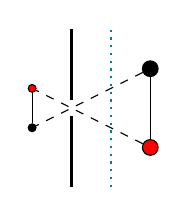
\begin{tikzpicture}[x=-1cm]
                        \draw[very thick]
                        (0, 0.1) -- (0, 1)
                        (0, -0.1) -- (0, -1);
                        \node[rbtb] (a0) at (-1, 0.5) {};
                        \node[rbtr] (b0) at (-1, -0.5) {};
                        \node[inner sep=1pt, circle, draw=black, fill=red] (a1) at (0.5, 0.25) {};
                        \node[inner sep=1pt, circle, draw=black, fill=black] (b1) at (0.5, -0.25) {};
                        \draw
                        (a0) -- (b0)
                        (a1) -- (b1);
                        \draw[dashed]
                        (a0) -- (b1)
                        (b0) -- (a1);
                        \draw[dotted, teal, thick] (-0.5, -1) -- (-0.5, 1);
                    \end{tikzpicture}
                \end{center}
                We want to model how $\vec{X} = (X, Y, Z)^\top$ is mapped to $\vec{x} = (x, y)^\top$ on the image plane.
                The image plane is rotated by 180 degrees and put as a \textbf{virtual} image plane in front of the pin hole (see the teal line above).
                This is more convenient, as the image is no longer flipped.
                \medskip

                The pinhole is treated as the camera origin, and the distance from the camera origin to the image plane is referred to as the focal length $f$.
                In one dimension, we can use \textbf{similar triangles};
                \begin{center}
                    \begin{tikzpicture}[x=1.5cm, y=1.5cm]
                        \draw
                        (0, 0) edge[-latex] (0, 1.5)
                        (0, 0) edge[-latex] (3.5, 0)
                        (0, 0) -- (3, 1)
                        (1.5, 0) edge[dashed, right] node {$f\frac{Y}{Z}$} (1.5, 0.5)
                        (3, 0) edge[dashed, right] node {$Y$} (3, 1);
                        \node at (0, -0.25) {$C$};
                        \node at (1.5, -0.25) {$f$};
                        \node at (3, -0.25) {$Z$};
                    \end{tikzpicture}
                \end{center}
                This therefore gives us the following mapping;
                $$(X, Y, Z) \to \left(f\frac{X}{Z}, f\frac{Y}{Z}\right)$$
                Homogeneous coordinates provide some convenience in geometry, as $(x, y, 1)$ represents the same point as $(kx, ky, k)$ for any non-zero $k$ (and similarly for 3D).
                In homogeneous coordinates, this becomes the following (see \textbf{CO317});
                $$(X, Y, Z, 1) \to \left(f\frac{X}{Z}, f\frac{Y}{Z}, 1\right) \text{ or } (fX, fY, Z)$$
                This is a perspective projection, where the object will appear smaller as the distance increases.
                Pinhole cameras can be generalised to lens cameras, which also has similar triangles along the central ray.
                The mapping for a pinhole camera can be represented in the following matrix notation;
                $$\begin{bmatrix}
                    X \\ Y \\ Z \\ 1
                \end{bmatrix} \to \begin{bmatrix}
                    fX \\ fY \\ Z
                \end{bmatrix} = \begin{bmatrix}
                    f & 0 & 0 & 0 \\
                    0 & f & 0 & 0 \\
                    0 & 0 & 1 & 0
                \end{bmatrix} \begin{bmatrix}
                    X \\ Y \\ Z \\ 1
                \end{bmatrix}$$
            \subsubsection*{Principal Point Offset}
                For example, in a CCD array, the image origin is typically defined at the bottom / top left, hence the image coordinate system's origin my differ from the \textbf{principal point} $\vec{p} = (p_x, p_y)$ (which would be in the centre of the image plane).
                To account for this shift, $(X, Y, Z, 1)$ should be mapped to $(f\frac{X}{Z} + p_x, f\frac{Y}{Z} + p_y, 1)$;
                $$\begin{bmatrix}
                    fX + p_xZ \\
                    fY + p_yZ \\
                    Z
                \end{bmatrix} = \begin{bmatrix}
                    f & 0 & p_x & 0 \\
                    0 & f & p_y & 0 \\
                    0 & 0 & 1 & 0
                \end{bmatrix} \begin{bmatrix}
                    X \\ Y \\ Z \\ 1
                \end{bmatrix}$$
                This can be written more concisely as follows;
                \begin{align*}
                    \mat{K} & = \begin{bmatrix}
                        f & 0 & p_x \\
                        0 & f & p_y \\
                        0 & 0 & 1
                    \end{bmatrix} \\
                    \vec{x} & = \begin{bmatrix}[c|c]
                        \mat{K} & \vec{0}
                    \end{bmatrix} \vec{X_\text{cam}}
                \end{align*}
            \subsubsection*{World Coordinate System}
                Note that we're currently working in the camera's coordinate system (which is defined within the camera itself).
                However, the camera is actually moving in the \textbf{world coordinate system}.
                We can simply subtract the translation $\vec{C}$, if only translation is involved.
                However, if there is also rotation, we need to factor in a 3D rotation matrix $\mat{R}$;
                $$\vec{X_\text{cam}} = \mat{R}(\vec{X} - \vec{C})$$
                Note that we are using \textbf{inhomogeneous coordinates} (no `1' at the end), hence $\vec{X} = (X, Y, Z)^\top$.
                Using homogeneous coordinates, we can write the transformation as;
                $$\underbrace{\begin{bmatrix}
                    X_\text{cam} \\
                    Y_\text{cam} \\
                    Z_\text{cam} \\
                    1
                \end{bmatrix}}_{\vec{X_\text{cam}}} = \begin{bmatrix}
                    \mat{R} & -\mat{R}\vec{C} \\
                    0 & 1
                \end{bmatrix} \underbrace{\begin{bmatrix}
                    X \\ Y \\ Z \\ 1
                \end{bmatrix}}_{\vec{X}}$$
            \subsubsection*{Camera Matrix}
                We first perform a mapping from the (homogenous) world coordinate ($\vec{X}$) to the camera coordinate ($\vec{X_\text{cam}}$), which is then mapped to the image coordinate ($\vec{x}$).
                Hence we have the following (note that the matrices in \violet{violet}, when multiplied together, is the \textbf{pinhole camera matrix});
                $$\vec{x} = \violet{\begin{bmatrix}
                    f & 0 & p_x & 0 \\
                    0 & f & p_y & 0 \\
                    0 & 0 & 1 & 0
                \end{bmatrix}} \underbrace{\violet{\begin{bmatrix}
                    \mat{R} & -\mat{R}\vec{C} \\
                    0 & 1
                \end{bmatrix}} \vec{X}}_{= \vec{X_\text{cam}}}$$
                Note that the camera matrix can be written more concisely as the following (the column of 0s removes the bottom row of the world transformation);
                $$\mat{P} = \begin{bmatrix}
                    f & 0 & p_x \\
                    0 & f & p_y \\
                    0 & 0 & 1
                \end{bmatrix} \begin{bmatrix}
                    \mat{R} & -\mat{R}\vec{C}
                \end{bmatrix} = \mat{K} \begin{bmatrix}[c|c]
                    \mat{R} & -\mat{R}\vec{C}
                \end{bmatrix} = \mat{K}\mat{R} \begin{bmatrix}[c|c]
                    \mat{I} & -\vec{C}
                \end{bmatrix}$$
                We have a total of 9 degrees of freedom (3 intrinsic (internal to the camera) parameters, $(f, p_x, p_y)$ and 6 extrinsic (world to camera, outside of the camera) parameters to describe the 3 for 3D rotation and 3 for 3D translation).
                \medskip

                Note that we're still representing the image coordinates in the same units as the camera coordinates (such as millimetres), however we want to have some conversion ratio $k_x, k_y$ (such as pixels per millimetre);
                $$\left(f\frac{X}{Z} + p_x, f\frac{Y}{Z} + p_y, 1\right) \text{ converted to } \underbrace{\left(k_x\left(f\frac{X}{Z} + p_x\right), k_y\left(f\frac{Y}{Z} + p_y\right), 1\right)}_{(\alpha_xX + x_0, \alpha_yY + y_0, 1)}$$
                This converts the camera matrix to the following;
                $$\mat{P} = \begin{bmatrix}
                    \alpha_x & 0 & x_0 \\
                    0 & \alpha_y & y_0 \\
                    0 & 0 & 1
                \end{bmatrix} \begin{bmatrix}
                    \mat{R} & -\mat{R}\vec{C}
                \end{bmatrix}$$
                However, $\alpha_x$ and $\alpha_y$ may differ, such that the pixels are \textbf{anisotropic} (such as rectangular pixels), leading to 10 degrees of freedom.
                This can be increased to 11 degrees of freedom when we account for skew (note that $s = 0$ for most cameras), when the axes are not orthogonal, giving us the most general camera matrix;
                $$\mat{P} = \begin{bmatrix}
                    \alpha_x & s & x_0 \\
                    0 & \alpha_y & y_0 \\
                    0 & 0 & 1
                \end{bmatrix} \begin{bmatrix}
                    \mat{R} & -\mat{R}\vec{C}
                \end{bmatrix}$$
            \subsubsection*{Calibration}
                Assume that we know the 3D structure, we want to estimate the camera matrix (photographer pose) from a 2D image.
                Given a set of points $\{\vec{X_i}, \vec{x_i}\}$, we want to estimate the matrix $\mat{P}$, which is similar to many problems previously encountered.
                We can either solve this as an (overdetermined) equation system, or to formulate this as an optimisation problem.
                \medskip

                This mapping is formulated as;
                $$\begin{bmatrix}
                    x \\ y \\ z
                \end{bmatrix} = \begin{bmatrix}
                    p_1 & p_2 & p_3 & p_4 \\
                    p_5 & p_6 & p_7 & p_8 \\
                    p_9 & p_10 & p_11 & p_12
                \end{bmatrix} \begin{bmatrix}
                    X \\ Y \\ Z \\ 1
                \end{bmatrix} = \begin{bmatrix}
                    \vec{p_1}^\top \\
                    \vec{p_2}^\top \\
                    \vec{p_3}^\top
                \end{bmatrix} \vec{X}$$
                The second form allows us to have the following;
                \begin{align*}
                    x & = \vec{p_1}^\top \vec{X} \\
                    y & = \vec{p_2}^\top \vec{X} \\
                    z & = \vec{p_3}^\top \vec{X}
                    \intertext{Converted into inhomogeneous image coordinates, we have;}
                    x & = \frac{\vec{p_1}^\top \vec{X}}{\vec{p_3}^\top \vec{X}} \\
                    y & = \frac{\vec{p_2}^\top \vec{X}}{\vec{p_3}^\top \vec{X}}
                \end{align*}
                Rearranged, we obtain the following two equations;
                $$\vec{p_1}^\top \vec{X} - \vec{p_3}^\top \vec{X}x = 0$$
                $$\vec{p_2}^\top \vec{X} - \vec{p_3}^\top \vec{X}y = 0$$
                By transposing both sides;
                $$\vec{X}^\top\vec{p_1} - \vec{X}^\top\vec{p_3}x = 0$$
                $$\vec{X}^\top\vec{p_2} - \vec{X}^\top\vec{p_3}y = 0$$
                This can now be written in matrix form, where $\vec{p_i}$ is a $4 \times 1$ vector;
                $$\underbrace{\begin{bmatrix}
                    \vec{X}^\top & 0 & -\vec{X}^\top x \\
                    0 & \vec{X}^\top & -\vec{X}^\top y
                \end{bmatrix}}_{2 \times 12} \underbrace{\begin{bmatrix}
                    \vec{p_1} \\
                    \vec{p_2} \\
                    \vec{p_3}
                \end{bmatrix}}_{12 \times 1} = \vec{0}$$
                For $n$ pairs of coordinates, the overdetermined system can be formed as follows;
                $$\underbrace{\begin{bmatrix}
                    \vec{X_1}^\top & 0 & -\vec{X_1}^\top x_1 \\
                    0 & \vec{X_1}^\top & -\vec{X_1}^\top y_1 \\
                    \vdots & \vdots & \vdots \\
                    \vec{X_n}^\top & 0 & -\vec{X_n}^\top x_n \\
                    0 & \vec{X_n}^\top & -\vec{X_n}^\top y_n
                \end{bmatrix}}_{2n \times 12} \underbrace{\begin{bmatrix}
                    \vec{p_1} \\
                    \vec{p_2} \\
                    \vec{p_3}
                \end{bmatrix}}_{12 \times 1} = \vec{0}$$
                Due to this form, the solution $\vec{p}$ is the null space of $\mat{A}$ (the large matrix) - this can be solved with the following optimisation problem, note that we add a constraint $|| \vec{p} ||^2 = 1$ as we want to exclude trivial solutions (where $\vec{p} = \vec{0}$);
                $$\vec{p} = \argmin_{\vec{p}} || \mat{A} \vec{p} ||^2$$
                This can be solved by performing singular value decomposition for the matrix $\mat{A}$ (see \textbf{CO233}), where $\mat{U}$ and $\mat{V}$ are orthogonal, and $\mat{\Sigma}$ is diagonal.
                $\vec{p}$ is the column of $\mat{V}$ corresponding to the \textbf{smallest singular value};
                $$\underbrace{\mat{A}}_{m \times n} = \underbrace{\mat{U}}_{m \times m}\underbrace{\mat{\Sigma}}_{m \times n}\underbrace{\mat{V}^\top}_{n \times n}$$
                Once we have this solution, w can rearrange the elements to form the camera matrix, establishing the mapping from 3D to 2D.
                \medskip

                We can obtain these data points (pairs of camera and image coordinates) with references objects (such as a checkerboard), which we can use to identify correspondences between points in the image and scene via a manual process.
                \medskip

                This can be used to relate information from the 3D world to 2D images, which is utilised in AR or object tracking for drones.
            \subsubsection*{Multiple View Geometry}
                We only consider a single perspective.
                However, if the camera is moved, multiple view geometry is used (where the image coordinates differ based on the perspective of the camera).
\end{document}